\documentclass[
  % oneside,
  twoside,
  degree=bachelor,
  field=science,
  fullwidthstop=circle,
  fontset=fandol,
  times=false,
  minted=false,
  biblatex=true,
]{tongjithesis}

% \tjbibresource{bib/note.bib}
\tjbibresource{bib/abbr.bib}
\tjbibresource{bib/references.bib}

\usepackage{xspace}
\usepackage[cal=cm]{mathalpha}

% 定理环境（补充原论文使用的完整名称别名）
\newtheorem{property}{性质}[chapter]
\newtheorem{theorem}{定理}[chapter]
\newtheorem{proposition}{命题}[chapter]
\newtheorem{lemma}{引理}[chapter]
\newtheorem{definition}{定义}[chapter]

% tikz 设置
\usetikzlibrary{calc}
\tikzset{
  timeaxis/.style={very thick, ->},
  flight/.style={thick, ->},
  timec/.style={dashed},
  timecActive/.style={ultra thick, ->},
  dot/.style={circle,fill=black,inner sep=1.2pt},
}

% ========== Sets ==========

% Planning horizon start
\newcommand{\planningStart}{\alpha}

% Planning horizon end
\newcommand{\planningEnd}{\beta}

% Time discretization step
\newcommand{\discretizationStep}{\Delta}

% Airport-specific initial discretization step (travel-time based)
\newcommand{\initStep}{s} % _{i}

% Check time
\newcommand{\checkTime}{t_c}

% Time discretization set
\newcommand{\discretization}{\mathcal{T}}

% Full time discretization set
\newcommand{\discretizationFull}{\hat{\discretization}}

%  ----------------- Network -------------------

% Flat Network $\netFlat=(\airportSet, \segSet)$
\newcommand{\netFlat}{\mathscr{G}}

% Set of airports
\newcommand{\airportSet}{\mathcal{I}}

% Set of segments indexed by $s$
\newcommand{\segSet}{\mathcal{S}}

% Distance for segment s
\newcommand{\distance}{D} % _{s}

% Time-Expanded Network $\net{\discretization}=(\nodeSet, \arcSet)$
\newcommand{\net}{\mathcal{G}} % {\discretization}

% Required frequency for segment s
\newcommand{\freq}{n} % _{s}

% Travel time for segment
\newcommand{\travelTime}{\tau} % _{s}

% Minimum interdeparture time
\newcommand{\minInterdepTime}{g} % _{s}

% Set of nodes
\newcommand{\nodeSet}{\mathcal{N}}

% Set of arcs
\newcommand{\arcSet}{\mathcal{A}}

% Flight arcs set notation
\newcommand{\flightArc}[1][{}]{{\arcSet^F_{#1}}}

% Departure arcs set notation
\newcommand{\departArc}{{\mathcal{D}}}

% Holding arcs set notation
\newcommand{\holdingArc}[1][{}]{{\arcSet^H_{#1}}}

% Holding incoming arcs
\newcommand{\holdingArcIn}{\mathcal{H}_{in}}

% Holding outcoming arcs
\newcommand{\holdingArcOut}{\mathcal{H}_{out}}

% Impossible departure numbers
\newcommand{\impDeparts}{Q}

% Red-eye arcs set notation
\newcommand{\redArc}{{\arcSet^R}}

% Serving arcs set notation
\newcommand{\servingArc}{{\arcSet^{S}}}

% Positioning arcs set notation
\newcommand{\positionArc}{{\arcSet^{P}}}

% Set of outgoing arcs from node (i,t)
\newcommand{\outArcSet}[1]{{\arcSet^{+}_{#1}}} % {i,t}

% Set of incoming arcs to node (i,t)
\newcommand{\inArcSet}[1]{{\arcSet^{-}_{#1}}} % {i,t}

% Set of flight arcs from node (i, $\cdot$) and fleet type is $f$
\newcommand{\outArcSetByF}[1]{{\arcSet^{+}_{#1}}} % {i,f}

% Set of flight arcs to node (i, $\cdot$) and fleet type is $f$
\newcommand{\inArcSetByF}[1]{{\arcSet^{-}_{#1}}} % {i,f}

% Set of holding arcs at time tc
\newcommand{\holdingArcTc}[1]{{\arcSet^H(#1)}} % {t_c}

% Set of flight arcs at time tc
\newcommand{\flightArcTc}[1]{{\arcSet^F(#1)}} % {t_c}

% Set of invert arcs at time tc
\newcommand{\invertArcTc}[1]{\overleftarrow{\arcSet}(#1)} % {t_c}

% Set of arcs for segment s at time t
\newcommand{\arcDuringSepTime}{D} % _{ijt}

% Aggregated departure flow in a separation window for segment (i,j) starting at t
\newcommand{\arcDepartFlow}{F^{\text{dep}}} % _{ijt}

% Number of flights which can depart in the interval $[t, t+\minInterdepTime_{ij})$
\newcommand{\departLimit}{\xi} % _{ijt}

% Combined Limit
\newcommand{\combLimit}{\bar{\xi}} % _{R}

% Set of arcs for segment s
\newcommand{\segArcSet}[1]{\arcSet(#1)} % {s}

% Segment of arc a
\newcommand{\sfa}[1]{s({#1})} % {a}

% Separation Violation Amount
\newcommand{\sepViolAmount}{V^{\text{sep}}} % _{ij}(t)

% Separation Violation Flow
\newcommand{\sepViolFlow}{N} % _{ijt}

% summation of the separation violation amount $\sepViolAmount_{ijt}$ and the illegal departure quantities $\impDeparts(i,t,f)$ and $\impDeparts(j,t,f)$
\newcommand{\sepInterViolAmount}{\mathscr{V}} % _{ijt}

% Cumulative Departures
\newcommand{\cumDepart}{D} % _{jf}(t)

% Cumulative Real Arrivals
\newcommand{\cumArrReal}{A^{\text{real}}} % _{jf}(t)

% Late Arrival Set
\newcommand{\lateArrSet}{\mathcal{A}_{\text{late}}}

% Discreted Path Signature of itinerary r
\newcommand{\pathSig}[1]{\pi({#1})} % {r}

% Equivalence class of itineraries by discreted path signature
\newcommand{\eqClassByPathSig}{S} % _{(R)}

% Equivalence relation by discreted path signature
\newcommand{\eqRelByPathSig}{\sim}

% Original Path of itinerary r
\newcommand{\origPath}[1]{\hat{\pi}({#1})} % {r}

% Equivalence class of itineraries by original path signature
\newcommand{\eqClassByOrigPath}{\mathscr{O}} % _{r'}^{r}

% Equivalence relation by original path signature
\newcommand{\eqRelByOrigPath}{\hat{\sim}}

% Itinerary Combination Set
\newcommand{\itinCombSet}{\mathscr{I}}

% Compatible Combination Set for super-itinerary R (optional method index)
\newcommand{\compatSet}[2][]{\mathcal{C}^{#1}(#2)} % [method]{R}

% Max Attraction Combination Set
\newcommand{\maxAttrCombSet}{\itinCombSet^{*}} % _{rp\ell}

%  ----------------- Market -------------------

% Set of markets
\newcommand{\marketSet}{\mathcal{M}}

% Set of passenger types
\newcommand{\psgTypeSet}{\mathcal{P}}

% Set of fare classes
\newcommand{\fareClassSet}{\mathcal{L}}

% Set of itineraries
\newcommand{\itinSet}{\mathcal{R}}

% Set of super-itineraries
\newcommand{\itinSetSuper}{\itinSet^{*}}

% Set of remaining super-itineraries
\newcommand{\remainingItienSetSuper}{\bar{\itinSetSuper}}

% Set of itineraries in market m
\newcommand{\itinInMarket}{R} % _{m}

% Set of super-itineraries in market m
\newcommand{\itinSuperInMarket}{R^{*}} % _{m}

% Set of itineraries in market m that use arc a
\newcommand{\itinUsingArc}[2]{R_{#1}(#2)} % {m}{a}

% Set of super-itineraries in market m that use arc a
\newcommand{\itinSuperUsingArc}[2]{R^{*}_{#1}(#2)} % {m}{a}

% Demand for market m and passenger type p
\newcommand{\demand}{D} % _{mp}

% Fare for itinerary r and fare class l
\newcommand{\fare}{TP} % _{r\ell}

% Outside attraction for market m and passenger type p
\newcommand{\outAttr}{\alpha^0} % _{mp}

% Attraction for itinerary r, passenger type p, fare class l
\newcommand{\attr}{\alpha} % _{rp\ell}

% Attraction for super-itinerary r, passenger type p, fare class l
\newcommand{\attrSuper}{\beta} % _{rp\ell}

% Adjusted attraction for outside option
\newcommand{\adjOutAttr}{\bar{\alpha}^0} % _{mp}

% Adjusted attraction for itinerary product
\newcommand{\adjAttr}{\bar{\attr}} % _{rp\ell}

% Adjusted attraction for super-itinerary product
\newcommand{\adjAttrSuper}{\bar{\attrSuper}} % _{rp\ell}

% Shadow attraction for outside option
\newcommand{\shadowOutAttr}{\omega^0} % _{mp}

% Shadow attraction for itinerary product
\newcommand{\shadowAttr}{\omega} % _{rp\ell}

% Minimum non-zero attraction value in market m for passenger type p
\newcommand{\attrMin}{\attr^{\min}} % _{mp}

% Scaling factor for attraction parameters in market m for passenger type p
\newcommand{\attrScale}{\sigma} % _{mp}

% ------------------ Supply--------------

% Set of fleets
\newcommand{\fleetSet}{\mathcal{F}}

% Fleet capacity
\newcommand{\fleetCap}{Q} % _{f}

% Operating cost for arc a and fleet f
\newcommand{\cost}{C} % _{af}

% Fleet availability
\newcommand{\fleetAvail}{\kappa} % _{f}

% % \textbf{Decision}: Passenger flow variable on itinerary network
% \newcommand{\psgFlowVar}{\rho} % _{rp\ell}^{a}

% % ========== Notation Helpers ==========

% % Time node representation
% \newcommand{\timeNode}[2]{(#1, #2)} % {i}{t}

% % Segment representation
% \newcommand{\seg}[2]{(#1, #2)} % {i}{j}

% % Time arc representation
% \newcommand{\timeArc}[4]{(#1, #2, #3, #4)} % {i}{t}{j}{t'}

% % Market-passenger key
% \newcommand{\marketPsgKey}[2]{(#1, #2)} % {m}{p}

% % Itinerary-passenger-fare key
% \newcommand{\itinPsgFareKey}[3]{(#1, #2, #3)} % {r}{p}{\ell}

% ------------------------- Modeling -------------------------

% Problem abbreviation
\newcommand{\problemName}{SN-CC}

% Problem abbreviation
\newcommand{\problemNotation}{\textbf{\problemName}}

% Algorithm abbreviation
\newcommand{\algoNotation}{IA-DR}

% Problem model in discretization $\discretization$
\newcommand{\model}[1]{\problemNotation({#1})} % {\discretization}

% FDM model
\newcommand{\fdm}{\textbf{FDM}}

% UBM model
\newcommand{\ubm}{\textbf{UBM}}

% % DPD model as a LBM of network $\full{\net}$
% \newcommand{\dpd}{\textbf{DPD}}

% % DPD fix model: re-positioning
% \newcommand{\dpdFix}[1]{\textbf{DPD-RP}({#1})} % {\solution, \positionArc, \holdingArc}

% solution
\newcommand{\solution}{\mathcal{X}}

% the big M
\newcommand{\bigMNotation}{M}

% the small value
\newcommand{\smallValue}{\epsilon}

% Routing plan of $\solution$
\newcommand{\routingPlan}{\mathscr{P}}

% route in fleet f
\newcommand{\route}[1]{\mathbf{p}^{#1}} % {f}

% route in fleet f index k
\newcommand{\pathInRoute}[2]{p_{#2}^{#1}} % {f}{k}

% how many planes using route $\pathInRoute{f}{k}$
\newcommand{\routeAmount}[1]{\Omega({#1})} % {\pathInRoute{f}{k}}

% Wrap number for route $\pathInRoute{f}{k}$
\newcommand{\wrapnum}{\varpi} % _{fk}

% Fleet count in the start of planning horizon at airport $i$ for fleet $f$
\newcommand{\fleetCountStartByI}{\lambda} % _{if}

% -------------------- Decision Variables --------------------

% \textbf{Decision}: Fleet assignment variable for arc $a$ and fleet $f$
\newcommand{\fleetAssignVar}{x} % _{af}

% \textbf{Decision}: Outside option market share variable
\newcommand{\outsideShareVar}{{w^0}} % _{mp}

% \textbf{Decision}: Itinerary-fare market share variable
\newcommand{\shareVar}{w} % _{rp\ell}

% \textbf{Decision}: Itinerary-fare market share bound variable
\newcommand{\shareSVar}{sw} % _{rp\ell}

% % \textbf{Decision}: Fleet assignment indicator variable for arc $a$ and fleet $f$
% \newcommand{\assignIndVar}{y} % _{af}

% % \textbf{Decision}: Time potential variable for node $(i,t)$ and fleet $f$
% \newcommand{\timePotVar}{u} % _{it}^f

% % \textbf{Decision}: Loop indicator variable for arc $a$ and fleet $f$
% \newcommand{\loopIndVar}{s} % _{a,f}

% % \textbf{Decision}: Number of idle flights for fleet $f$
% \newcommand{\idleFleetVar}{\hat{\kappa}} % _{f}

% -------------------- FDM --------------------

% \textbf{Decision}: Margin flight indicator variable for arc $a$ and airport $i$
\newcommand{\marginVar}{y} % _{ia}

% \textbf{Decision}: Connection indicator variable for arc $a$ and $a'$
\newcommand{\connectionVar}{z} % _{aa'}

% \textbf{Decision}: Actual depart time for arc $a$
\newcommand{\departTimeVar}{\gamma} % _{a}

% ignore 8
\newcommand{\full}[1]{%
  \begingroup % 开启一个局部作用域
    \renewcommand{\nodeSet}{\hat{\mathcal{N}}}
    \renewcommand{\arcSet}{\hat{\mathcal{A}}}
    \renewcommand{\net}{\hat{\mathcal{G}}}
    #1% 处理传入的内容
  \endgroup % 作用域结束，\node 自动变回原样
}

% ignore 14
\newcommand{\innerSetNotationFont}{\mathrm}
\newcommand{\innerArcSetNotation}{\innerSetNotationFont{A}}
\newcommand{\wrapSet}{\innerSetNotationFont{W}}
\newcommand{\wrapTc}{\innerSetNotationFont{H}}

\newcommand{\arcPosi}{{\innerArcSetNotation_{fk}^{\checkTime,+}}}
\newcommand{\arcNega}{{\innerArcSetNotation_{fk}^{\checkTime,-}}}
\newcommand{\arcNorm}{{\innerArcSetNotation_{fk}^{\checkTime,0}}}
\newcommand{\sign}{\varsigma}
\newcommand{\signPropositionConnectionNotation}{}
\newcommand{\slr}[1]{\textbf{0$\signPropositionConnectionNotation$1}({#1})}
\newcommand{\srl}[1]{\textbf{1$\signPropositionConnectionNotation$0}({#1})}
\newcommand{\srr}[1]{\textbf{1$\signPropositionConnectionNotation$1}({#1})}
\newcommand{\sll}[1]{\textbf{0$\signPropositionConnectionNotation$0}({#1})}

% ignore 1
\newcommand{\TBD}{\textbf{\color{red}To Be Done in future work.}}

\begin{document}

% ============================================================
%  文档类选项（在 main.tex 的 \documentclass[...]{tongjithesis} 中设置）
%  field=science    理工科（工科类、理科类，默认）— 章节编号：1 / 1.1 / 1.1.1
%  field=humanities 文科  （人文、法学、外语、艺术）        — 章节编号：一、/（一）/ 1.
%  经管类属社科：编号要求依理工，撰写依理工模版；26 届为过渡期，可选 science 或
%  humanities；自 27 届起统一使用 science。
% ============================================================

% ============================================================
%  封面信息
% ============================================================
\school{经济与管理学院}
\major{信息管理与信息系统}
\student{2253789}{张子越}
\thesistitle{考虑顾客选择的服务网络设计}{基于行程聚合与动态细化的精确优化方法}
\thesistitleeng{Service Network Design Considering Customer Choice}{An Exact Optimization Approach with Itinerary Aggregation and Dynamic Refinement}
\thesisadvisor{魏可佶\quad 副教授}
\thesisdate{\the\year}{\the\month}{\the\day} % 使用当前日期; 也可以自定义日期

% ============================================================
%  信息说明页
% ============================================================

% 成果类型（三选一）：
%   thesis      — 毕业论文，摘要
%   design      — 毕业设计（软件/创意/建筑等非工程设计类），摘要
%   engineering — 毕业设计（工程设计类），设计总说明
\infotype{thesis}

% 内容简述（请用300字以内简要概述）
\infoabstract{%
本文研究考虑顾客选择行为的服务网络设计问题，该问题由于候选行程集合规模爆炸并与其他变量耦合而难以求解。本文提出行程聚合与动态细化框架，该框架利用路径签名将候选行程集合聚合为紧凑的超级行程集合，在聚合网络上求解松弛模型获得下界，在完整网络上修复得到可行上界，并通过迭代细化保证有限收敛到全局最优。在真实航空排班实例上，超级行程聚合将142万条候选行程压缩至约21万条（减少85\%），框架在所有测试实例上均于5小时内达到低于1\%的最优性间隙，显著优于直接求解方法。
}

% 毕业设计：图纸数量与正文字数（成果类型为 design 或 engineering 时填写，两者须同时填写）
% \infodrawings{5}
% \infowordcount{15000}

% 毕业论文：正文总字数（成果类型为 thesis 时填写）
\infothesiswords{25681}

% 随附资料（每条用 \item 开头；不填则显示空白行）
\infomaterials{
  \item 附录
}

\MakeCover
\cleardoublepage
\MakeInfoPage
\cleardoublepage

\frontmatter
\MakeAbstract{
考虑旅客选择的服务网络设计刻画了服务运营决策与内生旅客需求之间的交互关系，但其混合整数规划在实际规模下难以求解。本文提出一种精确的行程聚合与动态细化框架（\algoNotation），通过一系列可处理的松弛问题与可行解修复过程求解该问题。该框架同时对物理时空网络和旅客行程空间进行聚合：具有相同聚合路径签名的原始行程被表示为超级行程，其吸引力取值被设计为支配可行的原始行程组合，同时避免标准时间聚合所导致的严重收入高估，由此提供有效且紧的下界。互补的上界模块固定聚合服务频率并引入行程割，在完整网络上恢复可行时刻表。当上下界解存在差异时，动态细化过程有针对性地插入时间点，消除时序违规、间隔不可行性和虚假收入。本文证明了该算法在有限次迭代内收敛到全局最优解。在真实航空实例上的计算实验表明，\algoNotation 能够求解此前不可处理的、含百万级行程变量的大规模模型，在实际可接受的计算时间内给出高质量的解。}{服务网络设计，旅客选择，行程聚合，混合整数规划，精确算法}

\MakeAbstractEng{
Service network design with passenger choice captures the interaction between service operations and endogenous passenger demand, but its mixed-integer formulation is computationally intractable at realistic scales. We propose an exact Itinerary Aggregation and Dynamic Refinement framework (\algoNotation) that solves this problem through a sequence of tractable relaxations and feasible repairs. The framework aggregates both the physical time-space network and the passenger itinerary space. Original itineraries with common aggregated path signatures are represented by super-itineraries, whose attraction values are chosen to dominate feasible original itinerary combinations while avoiding the severe revenue overestimation caused by standard temporal aggregation. This construction provides a valid and tight lower bound. A complementary upper-bound module fixes aggregate service frequencies and adds itinerary cuts to recover feasible schedules on the full network. Whenever the lower- and upper-bound solutions differ, a dynamic refinement procedure adds targeted time points to remove chronological violations, separation infeasibilities, and phantom revenue. We prove finite convergence of the resulting algorithm to a globally optimal solution. Experiments on real-world airline instances demonstrate that \algoNotation solves previously intractable large-scale models with up to millions of itinerary variables, producing certified high-quality solutions within practical runtime limits.}{Service Network Design, Passenger Choice, Itinerary Aggregation, Mixed-integer Programming, Exact Algorithm}


\clearpage
\tableofcontents
% \listoffigures   % 插图清单（根据需要取消注释）
% \listoftables    % 表格清单（根据需要取消注释）
\cleardoublepage

\mainmatter

% 绪论
\chapter{绪论}
\section{Introduction}
\label{sec:introduction}

Service Network Design (SND) is the problem of determining service plans---routes, schedules, and resource capacities---to satisfy transportation demand over a network. It occupies a central position in transportation planning and operations research, as the service plan dictates both the operating cost structure and the level of service experienced by customers. Foundational SND models cast the problem as a multi-commodity flow (MCF) optimization on time-space networks, where nodes represent locations at specific points in time and arcs represent either service operations or idle resource holding \citep{boland2017continuous}. The resulting mixed-integer programs (MIPs) must simultaneously determine which services to operate, when to operate them, and which resource types to assign, making SND one of the most challenging combinatorial optimization problems in practice.

A critical limitation of classical SND formulations is the assumption that demand is exogenous---fixed independently of the service plan. In reality, when travelers can choose among competing itineraries offered by one or more operators, or opt out of traveling entirely, the demand becomes endogenous: it depends on the service plan itself. Incorporating passenger choice models into SND creates a feedback loop between supply and demand decisions. The service plan determines the set of available itineraries, which in turn determines the demand captured, which in turn affects the profitability of the service plan. This coupling makes the problem significantly harder---the feasible region now includes choice-consistency constraints that link operational and demand variables---but also far more realistic and valuable for practical planning.

The integration of SND with passenger choice arises naturally in several transportation domains. In \textit{airline scheduling}, carriers jointly optimize fleet assignment, timetabling, and route planning while accounting for how passengers select among available itineraries based on schedule convenience, connection quality, and fare levels \citep{wei2020airline, yan2022choice}. In \textit{urban rail and metro operations}, transit agencies design train frequencies and stopping patterns on networks where commuters choose routes based on travel time, number of transfers, and crowding levels. In \textit{intercity bus and rail services}, operators plan service frequencies and departure schedules for corridors where travelers choose between competing operators and modes based on departure times, travel duration, and ticket price. Across all these settings, the core modeling challenge is the same: the combinatorial explosion of feasible itineraries over the time-space network, coupled with the need to endogenize demand through a discrete choice framework.

The standard modeling approach for SND with passenger choice formulates the problem as a multi-commodity flow program on a time-space network with an embedded discrete choice model. The planning horizon is discretized into time intervals, and service arcs are defined over this discretized network. Passenger demand is endogenized through the Sales-Based Linear Program (SBLP) linearization of the General Attraction Model (GAM) \citep{gallego2015general}, which provides a tractable linear representation of choice probabilities within the MIP. The resulting formulation simultaneously optimizes service operations (binary assignment of resources to arcs) and demand allocation (continuous market share variables governed by choice-consistency constraints). However, the model is extremely large: even for moderately sized networks, the number of feasible itineraries can reach hundreds of thousands, and the interaction between binary service variables and continuous choice variables produces a dense, ill-conditioned constraint matrix.

Existing solution methods face fundamental limitations when applied to this problem class. Dynamic Discretization Discovery (DDD), introduced by \citet{boland2017continuous}, efficiently compresses the time-space network by starting with a coarse discretization and iteratively refining only where needed, guaranteeing convergence to the continuous-time optimum. However, DDD was designed for freight and service network problems with exogenous demand; it lacks the mechanism to handle the itinerary-based passenger choice behavior that couples demand allocation to the service plan. Decomposition methods have been applied to improve the tractability of choice-based airline schedule-design models \citep{yan2022choice}. However, these approaches are primarily designed to produce high-quality heuristic solutions and do not provide an exact dynamic-refinement framework for the itinerary-level, resource-coupled formulation studied here. Direct MIP solving of the full formulation is intractable for realistic instances: the massive number of itinerary variables---potentially hundreds of thousands to millions---overwhelms commercial solvers, which stall in the branch-and-bound process due to weak LP relaxations and fractional degeneracy.

In this paper, we propose an exact solution framework that overcomes these limitations. Our main contributions are as follows:
\begin{enumerate}
    \item We develop an \textit{Itinerary Aggregation} technique that, combined with time discretization, produces a tight lower bound by constructing ``super-itineraries.'' These aggregated itineraries eliminate the fictitious revenue that arises from fractional resource allocations in the relaxed network, yielding a relaxation that is substantially tighter than the standard LP relaxation of the full model.
    \item We design a \textit{repair algorithm} for upper bound generation, based on frequency fixing and itinerary cuts, that reconstructs feasible integer solutions from the relaxed lower-bound solution. This structure-aware approach exploits the information embedded in the relaxation to produce high-quality feasible schedules.
    \item We propose a \textit{refinement strategy} that dynamically adds time points to the discretized network by detecting and resolving three types of relaxation artifacts---chronological violations, separation infeasibilities, and phantom revenue---guaranteeing finite convergence to the global optimum.
    \item We validate the framework on real-world instances, demonstrating that previously intractable problems with nearly half a million itinerary variables can be solved to provable optimality.
\end{enumerate}

The remainder of this paper is organized as follows. Section~\ref{sec:literature_review} reviews the relevant literature on service network design and dynamic discretization discovery. Section~\ref{sec:model_overview} formally describes the problem and presents the mathematical formulation on the full time-space network. Section~\ref{sec:algorithm} details the solution methodology, including the relaxation model that provides a valid lower bound (Section~\ref{sec:lbm}), the upper bound generation procedure (Section~\ref{sec:ub}), and the refinement strategy that guarantees convergence (Section~\ref{sec:refinement}). Section~\ref{sec:comp_study} presents the computational study, demonstrating the practical applicability of the framework. We conclude with a summary of findings and directions for future research.


% 文献综述与理论基础
\chapter{文献综述与理论基础}
\label{sec:foundation}
\section{数学规划与混合整数规划基础}

数学规划是运筹学的核心工具，用于在满足一组约束条件的前提下，寻找使目标函数取得最优值的决策方案。一个数学规划模型由三个基本要素构成：决策变量，描述决策者可以控制的量；目标函数，衡量决策方案优劣的准则；约束条件，刻画决策必须满足的限制。

根据决策变量的类型和约束的结构，数学规划可分为若干类别。线性规划（LP）要求目标函数和约束均为决策变量的线性函数，且变量取值连续\citep{bertsimas1997introduction}。整数规划（IP）在线性规划的基础上要求部分或全部变量取整数值，当所有变量均为整数时称为纯整数规划。混合整数规划（MIP）则同时包含连续变量和整数变量，是实际应用中最常见的形式\citep{wolsey1998integer, nemhauser1988integer}。一般的混合整数规划可以写成如下形式：
\begin{equation}
\begin{aligned}
\min \quad & c^\top x + d^\top y \\
\text{s.t.}\quad & Ax + By \ge b,\\
& x \ge 0,\\
& y \in \{0,1\}^n.
\end{aligned}
\label{eq:general_mip}
\end{equation}
其中$x$表示连续决策变量，$y$表示二元或整数决策变量，目标函数表示成本、收益或两者的组合，约束表示资源、容量、逻辑关系等限制。

为帮助理解 MIP 的结构，考虑一个固定费用网络设计问题的简化形式：
\begin{equation}
\begin{aligned}
\min \quad & \sum_{(i,j)\in A} F_{ij} y_{ij} + \sum_{(i,j)\in A} c_{ij} f_{ij} \\
\text{s.t.}\quad & \sum_{j:(i,j)\in A} f_{ij} - \sum_{j:(j,i)\in A} f_{ji} = b_i, \quad \forall i\in N,\\
& f_{ij} \le U_{ij}\, y_{ij}, \quad \forall (i,j)\in A,\\
& f_{ij}\ge 0,\quad y_{ij}\in\{0,1\}.
\end{aligned}
\label{eq:fcnd}
\end{equation}
其中$y_{ij}=1$表示弧$(i,j)$被开通，$f_{ij}$表示弧上的流量。约束$f_{ij}\le U_{ij}y_{ij}$是典型的连续流量变量与二元开通变量的耦合：只有弧被开通时流量才能为正。本文中的服务弧激活变量$x$与顾客选择份额$w$的耦合，本质上也属于这类 MIP 结构，只是更为复杂——因为需求不是外生给定的，而是由顾客选择内生产生的。例如，后文模型中的容量约束将顾客选择份额所诱导的客流量限制在已激活服务弧的座位容量之内，其作用与固定费用网络设计中的$f_{ij}\le U_{ij}y_{ij}$类似，都是通过整数变量控制连续流量变量的可行范围。

\section{网络流与服务网络设计}

网络流模型是描述资源在网络中流动的基本框架\citep{ahuja1993network}。一个网络由节点集合$N$和弧集合$A$构成，流在弧上传输并在节点处满足守恒条件。最小费用网络流问题的标准形式为：
\begin{equation}
\begin{aligned}
\min \quad & \sum_{(i,j)\in A} c_{ij} f_{ij}\\
\text{s.t.}\quad & \sum_{j:(i,j)\in A} f_{ij} - \sum_{j:(j,i)\in A} f_{ji} = b_i, \quad \forall i\in N,\\
& 0\le f_{ij}\le u_{ij}, \quad \forall (i,j)\in A.
\end{aligned}
\label{eq:mcf_basic}
\end{equation}
其中$b_i$为节点$i$的净供给量（正为供给，负为需求），$u_{ij}$为弧容量。当网络中存在多种商品（即多个起讫对的流量需求）时，每个商品$k$各自满足流守恒但共享弧容量，问题扩展为多商品流（MCF）问题。

服务网络设计（SND）在多商品流的基础上引入了服务选择决策\citep{magnanti1984network, crainic2000service}。与经典网络流问题中所有弧均可用不同，SND中的服务弧需要通过分配资源来激活——只有被激活的服务弧才能承载流量。因此，SND不仅要确定流量的路径分配，还要决定哪些服务弧被激活、以何种频率运营、分配何种类型的资源。这使得SND成为一个同时包含网络设计决策和流量分配决策的优化问题。

在本文的问题中，网络节点对应不同时间点的服务站点，服务弧对应计划中的服务班次，资源对应可分配的服务设备。运营商需要在资源总量、流守恒和运营约束下，确定最优的服务激活和资源分配方案。

从问题结构的递进关系来看，多商品流问题假设网络中所有弧均可用，只需确定流量分配；服务网络设计在此基础上引入服务激活决策，需要同时确定哪些弧可用以及流量如何分配；而考虑顾客选择的服务网络设计则进一步将需求从外生输入变为内生变量，使服务激活、资源分配和需求分配三者相互耦合。因此，从网络流到服务网络设计，再到考虑顾客选择的服务网络设计，问题复杂度的增加主要来自两个方面：一是服务开通决策引入整数变量；二是顾客选择行为使需求分配由外生参数变为内生变量。

\section{时空网络建模}

交通服务具有天然的时间维度：同一条线路在不同时间出发构成不同的服务选项。为在优化模型中精确表示这种时间结构，时空网络建模方法将规划时域离散化为若干时间点，并将空间网络在时间维度上展开。

具体而言，对于空间网络中的每个节点$i$和离散化后的每个时间点$t$，构造一个时空节点$(i,t)$。网络中的弧分为两类：服务弧连接不同空间节点在不同时间点的时空节点，表示从$(i,t)$出发、在$(j,t')$到达的一次服务运营，其中$t'-t$等于该服务的旅行时间；持有弧连接同一空间节点在相邻时间点的时空节点，表示资源在该节点的等待。如图~\ref{fig:time_space_network_basic}所示，空间节点$i$和$j$在不同时间点被复制为多个时空节点；从$(i,t_1)$到$(j,t_3)$的斜向弧表示一次服务运营，而同一空间节点相邻时间点之间的水平弧表示资源等待。

\begin{figure}[H]
\centering
\begin{tikzpicture}[scale=0.95,
    timepoint/.style={circle, fill=black, inner sep=1.6pt},
    service/.style={->, thick, blue!70!black},
    hold/.style={->, thick, gray!70},
    labelnode/.style={font=\small}]
% node labels
\node[labelnode] at (-0.6,1.6) {节点 $j$};
\node[labelnode] at (-0.6,0) {节点 $i$};
% time labels
\foreach \x/\t in {0/$t_1$,1.6/$t_2$,3.2/$t_3$,4.8/$t_4$,6.4/$t_5$} {
    \node[labelnode] at (\x,-0.45) {\t};
}
% time-space nodes
\foreach \x in {0,1.6,3.2,4.8,6.4} {
    \node[timepoint] at (\x,0) {};
    \node[timepoint] at (\x,1.6) {};
}
% holding arcs
\foreach \x/\xn in {0/1.6,1.6/3.2,3.2/4.8,4.8/6.4} {
    \draw[hold] (\x,0) -- (\xn,0);
    \draw[hold] (\x,1.6) -- (\xn,1.6);
}
% service arcs
\draw[service] (0,0) -- (3.2,1.6);
\draw[service] (1.6,0) -- (4.8,1.6);
\draw[service] (3.2,0) -- (6.4,1.6);
% annotations
\node[labelnode, blue!70!black] at (2.25,1.15) {服务弧};
\node[labelnode, gray!70!black] at (5.5,0.25) {持有弧};
\draw[->, blue!70!black, thin] (2.25,1.0) -- (1.5,0.75);
\draw[->, gray!70!black, thin] (5.5,0.15) -- (5.6,0.0);
\node[labelnode] at (3.2,-0.9) {时间};
\end{tikzpicture}
\caption{时空网络示意图}
\label{fig:time_space_network_basic}
\end{figure}

时空网络的优势在于将时间约束（如最小间隔时间、中转衔接时间）转化为网络结构约束，使得复杂的调度问题可以在统一的网络流框架下建模\citep{desrosiers1995time, zhu2014scheduled}。然而，时空网络的规模随时间分辨率的提高而快速增长：若空间网络有$n$个节点、离散化产生$T$个时间点，则时空网络包含$nT$个节点，弧的数量也相应增加。这种规模膨胀是本文需要解决的关键计算挑战之一\citep{boland2019price}。

\section{离散选择模型基础}

在经典的服务网络设计模型中，需求被视为外生给定的——每个起讫对的客流量固定，不受服务计划的影响。然而在客运场景中，需求是内生的：顾客会根据可用行程的服务属性进行选择。离散选择模型为描述这种选择行为提供了理论基础。

离散选择模型假设每位顾客面对一个有限的选择集合，集合中的每个方案具有一个效用值，由系统效用（可观测属性的函数）和随机误差项组成\citep{mcfadden1974conditional, benakiva1985discrete, train2009discrete}。顾客选择效用最高的方案。当随机误差项服从独立同分布的极值分布时，得到多项Logit（MNL）模型，其选择概率具有封闭的解析表达式：方案$i$被选择的概率正比于其吸引力$\alpha_i = \exp(V_i)$，其中$V_i$为系统效用。

在本文的问题中，每个市场中的顾客面对若干可行行程和一个外部选项（不出行）。外部选项的吸引力反映了顾客放弃出行的倾向。为了将选择行为嵌入线性优化模型，网络收入管理领域发展了基于选择的线性规划\citep{liu2008choice}和基于销售的线性规划（SBLP）\citep{gallego2015general}等框架，通过吸引力参数将非线性选择概率转化为线性约束。后续模型采用基于吸引力的线性表示，通过吸引力参数和选择一致性约束刻画顾客的需求分配行为。

\section{松弛、上下界与最优性间隙}

在混合整数规划求解中，直接获得全局最优解往往十分困难。为衡量一个可行解的质量，通常使用上界、下界和最优性间隙等概念。

对于最小化问题而言，任意可行解的目标函数值均可作为原问题最优值的上界；而若能够证明原问题的最优值不可能低于某一数值，则该数值称为下界。当上界与下界足够接近时，即可说明当前可行解已经接近最优。

松弛模型是构造下界的常用方法。其基本思想是放宽原问题中的部分约束，得到一个更容易求解的问题。由于松弛模型的可行域包含原问题的可行域，在最小化问题中，松弛模型的最优值不高于原问题最优值，因此可作为有效下界。另一方面，上界必须由原问题中的实际可行解给出。

本文后续提出的求解框架正是基于这一思想：首先在聚合网络和超级行程空间中求解松弛模型以获得下界；然后在完整网络上修复得到可行解以获得上界；最后通过上下界之间的差距判断当前解是否达到预设最优性容差。

在实际求解混合整数规划时，分支定界（Branch-and-Bound）是最常用的精确方法\citep{land1960automatic}。该方法通过系统地将问题分解为子问题（分支），并利用松弛模型的最优值对子问题进行剪枝（定界），逐步缩小搜索空间。在求解过程中，算法维护两个关键量：当前最好可行解的目标值（incumbent，即上界）和所有未探索子问题松弛值中的最小值（即下界）。二者之差的相对值称为最优性间隙（optimality gap），用于衡量当前解距离全局最优的程度。当间隙降至预设容差以下时，即可认为当前解已达到实际可接受的最优性水平。

当问题具有特殊的分块结构时，列生成（Column Generation）是另一种重要的精确求解技术\citep{desaulniers2005column, barnhart1998branch}。列生成通过将大规模线性规划分解为限制主问题和定价子问题，避免显式枚举所有变量，仅在需要时动态生成有改进潜力的列。当列生成与分支定界结合时，称为分支定价（Branch-and-Price），适用于变量数量极大的整数规划问题。

对于本文研究的大规模混合整数规划，由于行程变量数量庞大且线性松弛较弱，商业求解器的分支定界过程往往进展缓慢：每个节点的求解代价高，且松弛界改善有限。因此，本文不依赖通用分支定界直接求解完整模型，而是通过超级行程聚合构造更紧的松弛下界，并通过频率固定和收入约束在完整网络上高效生成可行上界，从而在框架层面实现间隙的快速收敛。

\section{Literature Review}
\label{sec:literature_review}

This section reviews three streams of literature that form the foundation of our work. The first concerns service network design (SND) formulations, tracing the evolution from cost-minimization models with exogenous demand to revenue-maximizing models that endogenize passenger choice. The second concerns passenger choice models and their integration into optimization frameworks. The third concerns dynamic discretization and iterative refinement methods for time-space network optimization.

\subsection{Service Network Design}

Service network design encompasses a broad class of optimization problems in which a planner determines which services to operate, when to schedule them, and how to allocate resources across a network to satisfy transportation demand. Foundational work on transportation network design and freight service network design established this perspective by formulating service selection, routing, and resource allocation decisions as fixed-charge and multi-commodity network design problems, often represented on time-expanded or time-space networks \citep{magnanti1984network, crainic1986multicommodity, crainic2000service, andersen2009service}. These formulations capture the temporal dimension of service operations through discretized time-space graphs, where nodes represent locations at specific time points and arcs represent service movements or idle resource holding. The resulting mixed-integer programs must balance operating costs against service quality, subject to resource conservation, capacity, and scheduling constraints.

A central challenge in SND is the representation of demand. Classical models treat demand as exogenous---fixed independently of the service plan---and focus on cost minimization for a given set of origin-destination flows \citep{crainic2000service, andersen2009service, boland2017continuous}. In this stream, the demand side is usually represented as a set of fixed commodities, while the optimization model determines the service frequencies, schedules, capacities, and asset movements required to move those commodities at minimum cost. However, in passenger transportation settings, demand is inherently endogenous: travelers choose among available itineraries based on service attributes such as travel time, number of connections, and schedule convenience. This observation has motivated a substantial body of work on integrating discrete choice models into network optimization.

The airline industry has been a primary application domain for SND with endogenous demand. Early contributions by \cite{abara1989applying} and \cite{hane1995fleet} modeled the fleet assignment problem as large-scale integer programs, assuming exogenous demand and fixed revenues. Recognizing that leg-based demand models fail to capture the network effects of passenger routing, \cite{barnhart2002itinerary} shifted the modeling paradigm to itinerary-based demand, enabling a more accurate representation of how passengers flow through hub-and-spoke networks. Subsequent refinements incorporated enhanced revenue modeling \citep{barnhart2009airline} and frequency competition to account for congestion effects \citep{vaze2012modeling}.

Building on these modeling advances, \cite{wei2020airline} formulated the joint timetabling and fleet assignment problem as a discrete-time service design problem with embedded passenger choice, solving it via an iterative heuristic. While this work demonstrated the revenue benefits of endogenizing demand, applying the model to full-scale instances involving major carriers presents substantial computational challenges due to the scale of the resulting time-space networks. Addressing these tractability concerns, \cite{yan2022choice} introduced a decomposition-based solution approach that reduces dimensionality while preserving choice characteristics, demonstrating consistent improvements over benchmark methods in both computational efficiency and solution quality. Nevertheless, existing approaches remain heuristic or decomposition-based and do not provide an exact framework with provable global optimality for the large-scale, itinerary-level formulation considered in this paper.

Despite these advances, the SND literature with endogenous demand has focused predominantly on airline applications. Although related planning problems in public transit and bus networks have been extensively studied under transit network design, bus network design, and frequency-setting frameworks \citep{ceder1986bus, guihaire2008transit, farahani2013review}, these studies typically emphasize route design, frequency setting, scheduling, and passenger assignment rather than an exact integration of itinerary-level discrete choice with resource-constrained service network design. This gap motivates our focus on an exact approach for service network design with passenger choice that preserves the operational coupling between service scheduling, resource assignment, and endogenous demand.

\subsection{Passenger Choice Models}

A key challenge in service network design with endogenous demand is the tractable representation of passenger choice behavior within optimization models. Discrete choice models provide the theoretical foundation for predicting how travelers select among competing alternatives based on service attributes. The Multinomial Logit (MNL) model, derived from random utility maximization, is the most widely used specification due to its closed-form choice probabilities and its tractability in estimation and optimization \citep{mcfadden1974conditional, benakiva1985discrete}. Nested logit models extend the MNL framework by allowing alternatives within the same nest to share unobserved utility components, thereby relaxing the strict independence of irrelevant alternatives property for similar alternatives such as itineraries with common legs, connection patterns, or departure-time characteristics \citep{mcfadden1978modeling, benakiva1985discrete}.

A key breakthrough in tractably embedding choice behavior into optimization models came from choice-based linear programming formulations in network revenue management \citep{liu2008choice}, the Sales-Based Linear Program (SBLP) of \cite{gallego2015general}, and the attractiveness-based formulations of \cite{di2014attractiveness}. These frameworks provide linear representations of choice-consistent demand allocation, enabling their integration into mixed-integer optimization models without directly carrying the nonlinear choice probabilities of classical logit formulations. The SBLP linearization of the General Attraction Model (GAM) is particularly useful because it models substitution and demand recapture through attraction parameters while retaining a compact linear structure. In contrast to simple attraction models that may overestimate recapture when preferred alternatives are unavailable, the GAM introduces adjusted attractions and shadow attractions to moderate substitution effects \citep{gallego2015general}. This feature makes the SBLP/GAM framework well suited for service design problems in which the set of offered itineraries is itself an endogenous outcome of the schedule.

The integration of these choice models with service network design remains computationally challenging. Choice-based formulations require itinerary-level variables and constraints, and the number of feasible itineraries can grow combinatorially with the size of the time-space network, the number of allowed connections, and the temporal resolution of the planning horizon. As a result, even when the choice model admits a linear representation, the resulting mixed-integer program may remain extremely large and weakly relaxed. Our work builds on the SBLP/GAM modeling framework, but addresses this algorithmic bottleneck through itinerary aggregation and iterative refinement.

\subsection{Dynamic Discretization and Iterative Refinement}

A persistent challenge in both general SND and its passenger-transportation variants is the representation of time. Traditional models rely on time-space networks that require a discretization of the planning horizon into fixed intervals. Coarse discretization compromises model accuracy by conflating services that operate at different times within the same interval, while fine discretization leads to an explosion in problem size, rendering large-scale instances intractable.

To address these limitations, \cite{boland2017continuous} introduced Dynamic Discretization Discovery (DDD) for the Continuous-Time Service Network Design Problem (CTSNDP). The CTSNDP formulates service scheduling in a continuous time domain, avoiding the approximation errors inherent in static discretization. The DDD algorithm starts with a coarse discretization and iteratively refines the time-space network by adding only the time points required to verify optimality or improve the solution. This allows the solver to work with a significantly smaller network than would be required by a uniformly fine static discretization, while theoretically guaranteeing convergence to the optimal solution of the continuous-time problem. The DDD framework represents a paradigm shift from ``construct-then-solve'' to ``construct-while-solving,'' and has proven effective for freight service network design where demand is exogenous and the primary challenge is temporal compression of the network.

However, when passenger choice is endogenized, the computational bottleneck shifts from the physical network to the logical passenger dimension. The number of feasible itineraries grows combinatorially with the temporal resolution, and the choice-consistency constraints tightly couple demand allocation across markets through shared service arcs. DDD, by design, addresses only the physical network compression and does not provide a mechanism for managing this itinerary-level explosion. Decomposition approaches \citep{yan2022choice} partially address the scale issue but sacrifice the coupling between markets.

In this paper, we adopt the general principle of iterative discretization refinement but depart from the DDD framework in a fundamental way. Rather than treating discretization refinement as the sole driver of convergence, we introduce itinerary aggregation as a complementary dimension of relaxation. By constructing super-itineraries that compactly represent equivalence classes of original itineraries, our approach simultaneously compresses both the physical network and the passenger demand space. The resulting framework---which we term the Itinerary Aggregation and Dynamic Refinement (\algoNotation)---produces tight lower bounds, generates feasible upper bounds via a structure-aware repair algorithm, and guarantees finite convergence to the global optimum through targeted refinement of both time points and itinerary partitions.


% 正文
\chapter{Problem Description}\label{sec:model_overview}

This study addresses a service network design problem that simultaneously considers service scheduling, resource assignment, and passenger choice behavior. Before presenting the mathematical formulations, we formally introduce the core terminology and parameters characterizing the problem.

\section{Concepts and Parameters}

A spatial origin-destination (OD) pair and its associated demand characterization define a market, denoted by the set $m \in \marketSet$. Within each market, the total passenger demand is initially given as $\demand_{mp}$ for different passenger types $p \in \psgTypeSet$ (e.g., business or leisure), representing differing utility preferences and travel urgencies. Furthermore, ticket offerings are divided into fare classes $\ell \in \fareClassSet$, capturing pricing structures.

The physical, time-independent trajectory between two nodes in the network is termed a spatial segment $s \in \segSet$. For each segment $s$, the operator typically dictates a predetermined number of required service operations $\freq_s$ across the planning horizon to maintain market presence. Additionally, to ensure stable operations, services departing on the same segment $s=(i,j)$ must obey a minimum separation time; we define $\arcDuringSepTime_{ijt}$ as the set of service arcs departing on segment $s$ within this separation interval starting from time $t$. The operator deploys a set of service resource types $f \in \fleetSet$. Each resource type has a restricted maximum available number of units $\fleetAvail_f$, alongside specific capacities $\fleetCap_{f}$ and operating costs.

To schedule services precisely, we represent the operation over a time-space network. While the time domain is continuous in reality, we computationally structure it using a discretization $\discretization$. A discretization defines a finite (and not necessarily uniform) set of time nodes for each spatial node in the network. Given a discretization $\discretization$, we establish a specific time-space network $\net = (\nodeSet, \arcSet)$ where $\nodeSet$ denotes the set of all time-space nodes and $\arcSet$ denotes the set of all time-space arcs under this temporal granularity. We respectively define $\outArcSet{i,t}$ and $\inArcSet{i,t}$ as the sets of time-space arcs departing from and arriving at a specific time-space node $(i, t)$. A time-space service arc $a \in \flightArc$ defines a specific service operation executed on a spatial segment $s$ with exact departure and arrival times drawn from the nodes in $\discretization$. The set of all service arcs associated with a segment $s$ is denoted as $\segArcSet{s}$. Similarly, resources remaining idle at a node between services are modeled by time-space holding arcs $a \in \holdingArc$. The total arc set $\arcSet$ is the union of service arcs and holding arcs, i.e., $\arcSet = \flightArc \uplus \holdingArc$. Finally, to monitor resource utilization, we track resources across the timeline: by picking an arbitrary snapshot count time $\checkTime$, we define $\flightArcTc{\checkTime}$ and $\holdingArcTc{\checkTime}$ as the respective sets of service arcs and holding arcs that cross this specific moment as follows:
\begin{equation}
    \flightArcTc{\checkTime} = 
    \{a=((i,t)\rightarrow(j,t^\prime))\;\forall a\in\flightArc\mid t\leq t_c<t^\prime\cup t^\prime<t\leq t_c<\beta\leq t+\travelTime_{ij}\}
    \label{def:main.flightArcTc}
\end{equation}
\begin{equation}
    \holdingArcTc{\checkTime} = 
    \{a=((i,t)\rightarrow(i,t^\prime))\;\forall a\in\holdingArc\mid t\leq t_c<t^\prime\cup t^\prime<t\leq t_c\}
    \label{def:main.holdingArcTc}
\end{equation}

The full discretization, denoted as $\discretizationFull$, represents the complete timeline formulated with a minimum standard temporal resolution $\discretizationStep$ (e.g., 5 minutes), containing every conceivable operational timing. The sets of graphs, nodes and arcs generated over this complete timeline represent the true, unrelaxed full problem space. By convention in this paper, when we discuss time-space networks, nodes or arcs (like $\net$, $\nodeSet$ or $\flightArc$) without a hat notation, they usually belong to a general, potentially reduced discretization $\discretization$. When we explicitly wish to refer to the sets under the full discretization $\discretizationFull$, we add a hat notation to the sets (e.g., $\full{\net}$, $\full{\flightArc}$ or $\full{\segArcSet{s}}$) to clearly differentiate the exact, original problem domain from any working subsets.

Passengers accomplish their travel by selecting an itinerary $r \in \itinSet$. Instead of being merely a series of spatial segments, an itinerary in our model is strictly defined as a chronological, connectable sequence of service arcs established over the full discretization $\discretizationFull$. The set of all valid itineraries serving market $m$ is denoted as $\itinInMarket_m$. If the operator's schedule provides no attractive or feasible itineraries, passengers drop out of the system by choosing the outside option.

To endogenously capture passenger choice behavior within the optimization framework, we adopt the Sales-Based Linear Program (SBLP) based on the General Attraction Model (GAM) proposed by \cite{gallego2015general}. In this context, the preference of a passenger type $p$ in market $m$ for a specific itinerary-fare combination $(r, \ell)$ is quantified by a deterministic nominal attraction parameter, denoted as $\attr_{rp\ell}$. Similarly, the outside option is assigned a nominal attraction value $\outAttr_{mp}$. These parameters are typically derived from discrete choice models, such as the Multinomial Logit (MNL) model, where $\attr_{rp\ell} = \exp(V_{rp\ell})$ where $V_{rp\ell}$ is the systematic utility of itinerary $r$ under fare class $\ell$ for passenger type $p$ in market $m$.

As demonstrated by \cite{gallego2015general}, standard attraction models (such as the Basic Attraction Model and the Multinomial
Logit Model) often overestimate the recapture rate when preferred options are unavailable. To address this, the GAM framework introduces the concept of shadow attractions to provide a more flexible representation of substitution behavior.
Following this framework, we define $\adjAttr_{rp\ell}$ as the adjusted attraction for itinerary $r$ under fare $\ell$, and $\adjOutAttr_{mp}$ as the adjusted attraction for the outside option.

According to the GAM definition, the adjusted attraction $\adjAttr_{rp\ell}$ represents the nominal attraction reduced by the corresponding shadow attraction $\shadowAttr_{rp\ell}$, i.e., $\adjAttr_{rp\ell} = \attr_{rp\ell} - \shadowAttr_{rp\ell}$. Therefore $0 \le \adjAttr_{rp\ell} \le \attr_{rp\ell}$. Conversely, the adjusted outside attraction $\adjOutAttr_{mp} = \outAttr_{mp} + \sum_{r\in \itinSet}\sum_{\ell\in \fareClassSet} \shadowAttr_{rp\ell}$, satisfying $\adjOutAttr_{mp} \ge \outAttr_{mp}$. These adjusted parameters are then directly employed in the demand balance constraints of the SBLP formulation to accurately model spill and recapture effects.

\section{Baseline Mathematical Model}

To formulate the problem mathematically, we introduce the following main decision variables representing service operations and passenger choices.

The primary operational decision captures the assignment of service resources over the time-space network. We define $\fleetAssignVar_{af}$ as the number of type-$f$ resources ($f \in \fleetSet$) assigned to traverse arc $a \in \arcSet$. For a service arc $a \in \flightArc$, $\fleetAssignVar_{af} \in \{0, 1\}$ acts as a binary variable indicating whether that specific service is operated by resource type $f$. For a holding arc $a \in \holdingArc$, $\fleetAssignVar_{af} \ge 0$ is a continuous variable representing the number of idle resources waiting at a node.

Additionally, to capture market demand fulfillment, we define $\shareVar_{rp\ell} \ge 0$ as the number of passengers of type $p \in \psgTypeSet$ within market $m$ that book itinerary $r \in \itinInMarket_{m}$ under fare class $\ell \in \fareClassSet$. Correspondingly, $\outsideShareVar_{mp} \ge 0$ represents the volume of passengers of type $p$ in market $m$ selecting the ``outside option'' (i.e., not purchasing any service from the operator).

\section{Mathematical Formulation}

We adopt the mathematical formulation $\model{\discretizationFull}$ proposed by \citet{wei2020airline} for the integrated service network design problem with passenger choice. This model simultaneously optimizes resource assignment decisions and passenger demand allocation under a discrete-choice framework, capturing the interdependencies between operational scheduling and revenue generation.

\full{
\noindent\textbf{Objective Function}
\begin{equation}
    \min \;\; 
    \sum_{a\in \flightArc}\sum_{f\in \fleetSet} \cost_{af}\, \fleetAssignVar_{af}
    \;-\;
    \sum_{m\in \marketSet}\sum_{p\in \psgTypeSet}\sum_{r\in \itinInMarket_{m}}\sum_{\ell\in \fareClassSet} 
    \demand_{mp}\,\fare_{r\ell}\, \shareVar_{rp\ell}
    % temp-command \tag{1a}
    \label{objfun:main}
\end{equation}
\noindent\textbf{Resource Assignment Constraints}
\begin{equation}
  \sum_{a\in \outArcSet{i,t}} \fleetAssignVar_{af} - \sum_{a\in \inArcSet{i,t}} \fleetAssignVar_{af} = 0 
  \quad \forall (i,t)\in \nodeSet,\; \forall f\in \fleetSet
  % temp-command \tag{1b}
  \label{constr:main.flow}
\end{equation}
\begin{equation}
    \sum_{a\in \holdingArcTc{\checkTime}} \fleetAssignVar_{af} + \sum_{a\in \flightArcTc{\checkTime}} \fleetAssignVar_{af} \le \fleetAvail_{f}
    \quad \forall f\in \fleetSet
    % temp-command \tag{1c}
    \label{constr:main.fleet_available}
\end{equation}
\noindent\textbf{Service Frequency Constraints}
\begin{equation}
    \sum_{f\in \fleetSet}\sum_{a\in \arcDuringSepTime_{ijt}} \fleetAssignVar_{af} \le 1 
    \quad \forall (i,j)\in \segSet,\; \forall t \in \discretization_i
    % temp-command \tag{1d}
    \label{constr:main.cooldown}
\end{equation}
\begin{equation}
    \sum_{f\in \fleetSet}\sum_{a\in \segArcSet{s}} \fleetAssignVar_{af} = \freq_{s}
    \quad \forall s\in \segSet
    % temp-command \tag{1e}
    \label{constr:main.seg_freq}
\end{equation}
\noindent\textbf{Passenger Choice Constraints}
\begin{equation}
    \outAttr_{mp}\, \shareVar_{rp\ell} \;\le\; \attr_{rp\ell}\, \outsideShareVar_{mp}
    \quad \forall m\in \marketSet,\, \forall p\in \psgTypeSet,\, \forall r\in \itinInMarket_{m},\, \forall \ell\in \fareClassSet
    % temp-command \tag{1f}
    \label{constr:main.choice.ratio}
\end{equation}
\begin{equation}
    \left(\frac{\adjOutAttr_{mp}}{\outAttr_{mp}}\right) \outsideShareVar_{mp}
    \;+\;
    \sum_{r\in \itinInMarket_{m}}\sum_{\ell\in \fareClassSet} 
    \left(\frac{\adjAttr_{rp\ell}}{\attr_{rp\ell}}\right) \shareVar_{rp\ell}
    \;=\; 1
    \quad \forall m\in \marketSet,\; \forall p\in \psgTypeSet
    % temp-command \tag{1g}
    \label{constr:main.choice.limit}
\end{equation}
\noindent\textbf{Capacity and Availability Constraints}
\begin{equation}
    \sum_{m\in \marketSet}\sum_{p\in \psgTypeSet}\sum_{\ell\in \fareClassSet}\sum_{r\in \itinUsingArc{m}{a}} 
    \demand_{mp}\, \shareVar_{rp\ell}\;\le\; \sum_{f\in \fleetSet} \fleetCap_{f}\, \fleetAssignVar_{af}
    \quad \forall a\in \flightArc
    % temp-command \tag{1h}
    \label{constr:main.choice.capacity}
\end{equation}
\begin{equation}
    \sum_{f\in \fleetSet} \fleetAssignVar_{af} \;\ge\; \shareVar_{rp\ell}
    \quad \forall a\in \flightArc,\; \forall m\in \marketSet,\, \forall r\in \itinUsingArc{m}{a},\, \forall p\in \psgTypeSet,\,\forall \ell\in\fareClassSet
    % temp-command \tag{1i}
    \label{constr:main.choice.covering}
\end{equation}
\noindent\textbf{Variable Domains}
\begin{equation}
    \fleetAssignVar_{af}\in\{0,1\} \quad \forall a\in \flightArc, \; \forall f\in \fleetSet
    % temp-command \tag{1j}
    \label{constr:main.domain.x.flight}
\end{equation}
\begin{equation}
    \fleetAssignVar_{af}\ge 0 \quad \forall a\in \holdingArc, \; \forall f\in \fleetSet
    % temp-command \tag{1k}
    \label{constr:main.domain.x.holding}
\end{equation}
\begin{equation}
    \outsideShareVar_{mp}\ge 0 \quad \forall m\in \marketSet, \; \forall p\in \psgTypeSet
    % temp-command \tag{1l}
    \label{constr:main.domain.w.out}
\end{equation}
\begin{equation}
    \shareVar_{rp\ell}\ge 0 \quad \forall r\in \itinSet, \; \forall p\in \psgTypeSet, \; \forall \ell\in \fareClassSet
    % temp-command \tag{1m}
    \label{constr:main.domain.w}
\end{equation}
}

The model defines a comprehensive plan matching services to passenger itineraries under resource and time constraints. The objective function \eqref{objfun:main} minimizes the total operating cost minus the total ticket revenue, effectively maximizing the operator's overall profit. For resource assignment, constraint \eqref{constr:main.flow} ensures flow conservation, meaning the number of type-$f$ resources arriving at any time-space node $(i, t)$ exactly equals those departing. Constraint \eqref{constr:main.fleet_available} bounds the resource utilization, ensuring that the total number of resources engaged in services ($\flightArcTc{\checkTime}$) and holdings ($\holdingArcTc{\checkTime}$) crossing a designated count time $\checkTime$ does not exceed the available resource limit $\fleetAvail_f$. To manage operational density, let $\arcDuringSepTime_{ijt} = \{a=((i,t^\prime)\rightarrow(j,t^{\prime\prime}))\;\forall a\in\flightArc\mid t\leq t^\prime<t+\minInterdepTime_{ij} \}$ denote the set of service arcs departing on segment $s=(i,j)$ within the minimum separation time starting from time $t$. Then constraint \eqref{constr:main.cooldown} enforces a minimum departure separation time, preventing multiple services from departing on the same spatial segment $(i,j)$ within the duration specified by the set $\arcDuringSepTime_{ijt}$, while constraint \eqref{constr:main.seg_freq} forces the schedule to exactly meet the required predetermined operation frequency $\freq_s$ for each segment $s$. Constraints \eqref{constr:main.choice.ratio}-\eqref{constr:main.choice.covering} represent the passenger choice constraints. Finally, constraints \eqref{constr:main.domain.x.flight} to \eqref{constr:main.domain.w} restrict the resource assignment and passenger allocation variables to their appropriate domains.

\section{Computational Complexity and Scale}\label{sec:complexity}\label{sec:preconditioning}

The \problemName problem is NP-hard. To see this, consider a restricted version in which passenger choice is removed: each market has fixed demand, a single admissible itinerary, and fixed revenue, and the choice-consistency constraints \eqref{constr:main.choice.ratio}--\eqref{constr:main.choice.limit} are inactive. The remaining problem is a service network design problem on a time-space network with binary service-activation and resource-assignment decisions subject to capacity and flow-balance constraints. This class contains the capacitated fixed-charge multicommodity network design problem as a special case, which is known to be NP-hard. Therefore, \problemName, which generalizes this restricted problem by adding itinerary-level choice variables and choice-consistency constraints, is NP-hard.

A central challenge lies in the combinatorial explosion of feasible itineraries. Each market admits a set of itineraries composed of one or more service arcs connected at intermediate nodes. The number of such itineraries grows rapidly with network size, the number of allowed connections, and the temporal resolution of the discretization. Consider a network with $|\airportSet|$ nodes and $|\segSet|$ directed segments. Under a discretization step of $\discretizationStep$ minutes over a 24-hour planning horizon, each segment admits up to $\lfloor 24 \times 60 / \discretizationStep \rfloor$ candidate departure times. For multi-leg itineraries with up to $k$ connections and a maximum connection window of $W$ minutes, the number of feasible itineraries scales combinatorially: each additional leg multiplies the possibilities by the number of compatible onward departures within the connection window. The exact count depends on the network topology, segment frequencies, connection-time rules, and the OD market set.

To illustrate, we consider a real-world airline scheduling instance that will be detailed in Section~\ref{sec:comp_study}. This network contains $60$ airports and $259$ directed segments. With a $15$-minute discretization, up to $2$ connections, and a $3$-hour maximum connection window, the enumeration yields $475{,}776$ feasible itineraries across the OD markets. Coupling this many itinerary variables with binary resource assignment constraints produces an extremely dense mixed-integer program that pushes the limits of state-of-the-art solvers.

Beyond worst-case complexity and practical scale, the formulation also presents numerical challenges. While the SBLP formulation elegantly linearizes the choice probabilities, directly feeding the raw attraction values (e.g., $\attr_{rp\ell}$) derived from discrete choice models into the solver can lead to severe numerical intractability. Specifically, in a typical Multinomial Logit (MNL) computation $\attr_{rp\ell} = \exp(V_{rp\ell})$, the raw attraction values are often exponentially small when the systematic utility $V_{rp\ell}$ is negative. This introduces extremely tiny coefficients into the constraint matrix, particularly in the choice ratio constraint \eqref{constr:main.choice.ratio}. As a consequence, the resulting constraint matrix becomes highly ill-conditioned, leading to numerical instability in the simplex method and severe tail-off effects during bound computation.
% \clearpage


\chapter{求解方法}\label{sec:solution_methodology}

\section{总体求解算法}
\label{sec:algorithm}

如第~\ref{sec:complexity}~节所讨论的，完整的\problemName 公式是NP-难的，由于时空网络和行程选择层的组合增长，在实践中变得计算困难。虽然标准的动态离散化发现（DDD）方法高效地压缩物理网络节点和弧，但它缺乏处理高度耦合的基于行程的旅客选择行为的机制。为弥合这一差距，我们提出行程聚合与动态细化（\algoNotation）。与标准DDD的根本区别在于，\algoNotation 将动态聚合从物理网络维度扩展到逻辑旅客维度。通过引入路径签名的概念，\algoNotation 将数百万条组成行程分组为紧凑的超级行程集合，而不丧失选择模型的结构完整性和解的最优性。通过这种双重聚合建立紧的下界、恢复逻辑有效的上界，以及精确插入缺失的时间点以纠正物理时序违规和行程级虚假收入，该算法框架保证收敛到精确的全局最优解。

本节概述了这一完整的精确求解框架，为三个基本算法构建模块奠定基础：提供有效下界的松弛模型（第~\ref{sec:lbm}~节）、作为修复算法的上界生成过程（第~\ref{sec:ub}~节）以及确保在迭代中收敛到全局最优的离散化细化策略（第~\ref{sec:refinement}~节）。

\subsection{初始离散化}\label{sec:initial_discretization}

\algoNotation 算法从一个刻意粗糙的初始离散化$\discretization$开始，以保持松弛模型的小规模。然而，初始步长的选择对松弛质量有深远影响。如第~\ref{sec:lbm}~节将详细介绍的，用于在松弛网络中构造服务弧的下取整映射规则（性质~\ref{def:relax.flightArc}）在网格相对于航段旅行时间过于粗糙时可能产生物理上无意义的逆弧。为从一开始就消除这种病态，我们采用一种初始离散化，其中每个节点$i \in \airportSet$获得一个根据其最短入站旅行时间校准的个体步长$\initStep_i$。精确的构造及其理论证明在第~\ref{sec:init_disc_detail}~节中给出。

\subsection{迭代框架}
我们从初始离散化开始，迭代求解下界模型以获得松弛解及其对应的下界。然后，我们使用松弛解通过基于MIP的修复算法生成上界。如果上界和下界之间的间隙在预定义阈值$\epsilon>0$内，则终止算法。否则，我们根据当前解细化离散化并重复该过程，这确保收敛到完整模型的全局最优解。算法总结在算法~\ref{alg:refinement}中。

\begin{algorithm}[ht]
\caption{Iterative Refinement Algorithm for $\problemNotation$}
\label{alg:refinement}
\begin{algorithmic}[1]
\State $LB \gets -\infty$.
\State $UB \gets +\infty$.
\State $\solution^{*} \gets \text{null}$.
\ForAll{$i\in\airportSet$}
\Comment{Initialize (Section~\ref{sec:initial_discretization})}
    \State $\initStep_i\gets\min_{j:(j,i)\in\segSet}\{\travelTime_{ji}\}$
    \State $\discretization_i\gets\{t\mid t=\planningStart+k\,\initStep_i,\, k \in \mathbb{Z}_{\ge0}, t < \planningEnd\}$
\EndFor
\State $iter\gets 0$
\Loop
    \State $iter \gets iter + 1$
    \State $\solution, LB \gets\Call{ATF}{\arcSet}$
    \Comment{Update Lower Bound}
    \State $\solution^{*}_{new}, UB_{new} \gets \Call{UB\_Model}{\solution}$
    \If{$UB_{new} < UB$}
        \State $\solution^{*}, UB \gets \solution^{*}_{new}, UB_{new}$
        \Comment{Update Upper Bound}
    \EndIf
    \If{$UB - LB \le \epsilon \;\textbf{or}\; iter \ge \text{maxIter}$}
        \State \textbf{break}
    \EndIf
    % \ForAll{$i \in \airportSet, t \in \discretization_i, f \in \fleetSet$}
    %     \Comment{Refinement}
    %     \State $Q_{imp} \gets D(i, t, f) - H_{in}(i, t, f) - A_{legal}(i, t, f)$
    %     \If{$Q_{imp} > 0$}
    %         \State $\mathcal{K} \gets A_{illegal}(i, t, f)$
    %         \State Sort $\mathcal{K}$ by flow volume $\fleetAssignVar_{k}$ in descending order
    %         \State $covered \gets 0$
    %         \ForAll{$k \in \mathcal{K}$}
    %             \If{$covered < Q_{imp}$}
    %                 \State $\discretization_i \gets \discretization_i \cup \{t_{\text{dep}}(k) + \travelTime_k\}$
    %                 \State $covered \gets covered + \fleetAssignVar_{k}$
    %             \Else
    %                 \State \textbf{break}
    %             \EndIf
    %         \EndFor
    %     \EndIf
    % \EndFor
    \State $\discretization \gets \Call{Refinement}{\solution, \discretization}$
    \Comment{Refine Discretization}
\EndLoop
\State \Return $\solution, \solution^{*}, LB, UB$
\end{algorithmic}
\end{algorithm}

\section{吸引力平衡预处理}\label{sec:preconditioning_solution}

为稳定优化过程，我们提出一种市场特定的数值预处理技术，称为吸引力平衡。对于每个市场$m \in \marketSet$和旅客类型$p \in \psgTypeSet$，我们在所有吸引力相关参数中识别最小非零绝对吸引力值：
\begin{equation*}
    \attrMin_{mp} = \min \left\{ \left|\outAttr_{mp}\right|, \, \left|\attr_{rp\ell}\right|, \, \left|\adjAttr_{rp\ell}\right| \mid r \in \itinInMarket_m, \, \ell \in \fareClassSet, \, \text{value} \neq 0 \right\}
    \label{eq:attr_min}
\end{equation*}

然后我们应用缩放因子$\attrScale_{mp} = 1.0 / \attrMin_{mp}$来均匀缩放该市场-旅客组合内的所有吸引力参数。由于根据GAM定义$\adjAttr_{rp\ell} = \attr_{rp\ell} - \shadowAttr_{rp\ell}$，我们缩放底层的名义吸引力和影子吸引力：
\begin{equation*}
\begin{aligned}
    \outAttr_{mp} &\leftarrow \attrScale_{mp} \cdot \outAttr_{mp}\\
    \attr_{rp\ell} &\leftarrow \attrScale_{mp} \cdot \attr_{rp\ell} \quad \forall r \in \itinInMarket_m, \, \ell \in \fareClassSet\\
    \shadowAttr_{rp\ell} &\leftarrow \attrScale_{mp} \cdot \shadowAttr_{rp\ell} \quad \forall r \in \itinInMarket_m, \, \ell \in \fareClassSet
\end{aligned}
\end{equation*}
因此，调整吸引力也按相同因子缩放，即$\adjAttr_{rp\ell} \leftarrow \attrScale_{mp} \cdot \adjAttr_{rp\ell}$和$\adjOutAttr_{mp} \leftarrow \attrScale_{mp} \cdot \adjOutAttr_{mp}$。

从数学上看，由于选择约束\eqref{constr:main.choice.ratio}和\eqref{constr:main.choice.limit}在每个市场-旅客组合内对吸引力参数是齐次的，将所有吸引力值乘以正常数$\attrScale_{mp}$严格保持可行域和最优解。为验证这一点，观察约束\eqref{constr:main.choice.ratio}变为：
\begin{equation*}
    (\attrScale_{mp} \cdot \outAttr_{mp})\, \shareVar_{rp\ell} \;\le\; (\attrScale_{mp} \cdot \attr_{rp\ell})\, \outsideShareVar_{mp}
\end{equation*}
这在从两边消去公共正因子$\attrScale_{mp}$后等价于原始约束。类似地，约束\eqref{constr:main.choice.limit}仍然有效，因为系数中的分子和分母按相同因子缩放，保持了比率$\adjAttr_{rp\ell}/\attr_{rp\ell}$和$\adjOutAttr_{mp}/\outAttr_{mp}$。

在计算上，这种预处理确保选择约束中最小的非零系数恰好为$1.0$，有效消除了矩阵病态。这一简单但关键的变换在我们求解框架的下界模型和上界模型组件中都起到催化剂作用，大幅加速了下界的收敛并增强了整体算法稳定性。本文报告的所有实验结果均在所有实例上统一采用了这一吸引力平衡预处理步骤。

一种解决数值不稳定性的替代方法是将$\shareVar_{rp\ell}$替换为$\demand_{mp} \shareVar_{rp\ell}$，其中唯一的$m$满足$r\in \itinInMarket_m$，并从目标函数和约束中移除$\demand_{mp}$。同时，$\shareVar_{rp\ell}$和$\outsideShareVar_{mp}$的域变为$[0, \demand_{mp}]$（或简单地$[0,+\infty]$）。这种方法可以有效消除目标函数和选择约束中的大系数，特别是$\demand_{mp}\fare_{r\ell}$项。新$\shareVar$变量的值表示选择行程$r$在票价$\ell$下的实际旅客数量，而非需求份额，后者通常是$[10^{-5}, 10^{-4}]$中的小分数。

\section{Relaxation Model $\model{\discretization, \itinSetSuper}$ via Discritization and Itinerary Aggregation}
\label{sec:lbm}

To address the tractability issues of the full time-space network, we introduce a time relaxation approach. The central idea of this step is to formulate a relaxed model on a much coarser, partially discretized time-space network, thereby drastically reducing the problem size while still guaranteeing a valid theoretical lower bound for the exact algorithm. This base model ignores certain strict timing feasibility requirements which are subsequently resolved in later algorithm stages. The model proposed in this section is called the Lower Bound Model (LBM) or the relaxation model in the rest of the paper.

% \section*{Understanding $\discretization$}
We consider $\discretization$ as a transformation of $\discretizationFull$. The transformation can be seen as aggregations of time-arcs. 
Every time-arc in $\full{\net}$ have a corresponding arc in $\net$.That means, we have some time-nodes $(i,t)$ in $\discretization$. All time-arcs $\full{\net}$ will exist in $\net$, and their start time, end time, and travel time may change because they can only use time-nodes in $\discretization$. In order to ensure the optimality, we can let the travel time be shorter than what they are. And there may even be inverse arcs whose start time is later than finish time.
The time-expanded network $\net = (\nodeSet, \arcSet)$, where $\nodeSet = \{(i,t)\mid \forall i\in\airportSet, t\in\discretization_i\},\;\arcSet = \holdingArc \cup \flightArc$, constructed from time discretization $\discretization$ satisfies the following properties:
% \[
%     \net = (\nodeSet, \arcSet)
% \]
% \[
%     \nodeSet = \{(i,t)\mid \forall i\in\airportSet, t\in\discretization_i\},\;\arcSet = \holdingArc \cup \flightArc
% \]
% \[
%     \net = \Phi(\netFlat, \discretization) = \Phi(\airportSet,\segSet,\discretization)
% \]
\begin{property}[Domain of Discretization $\discretization$]
    $\forall i\in\airportSet,\,\{\planningStart\}\subseteq\discretization_i\subseteq\discretizationFull_i$
\end{property}
\begin{property}[Nodes $\nodeSet = \Phi_{\nodeSet}(\netFlat, \discretization)$]
    Node set $N$ contains node $(i,\planningStart)\;\forall i\in\airportSet$
\end{property}
\begin{property}[Holding Arcs]
    \label{def:relax.holdingArc}
    Each ground arc $a\in\holdingArc$ is defined as $a=((i,t),(i,t^{+}))$, where
    $$t^{+}=\begin{cases}
            \min\{\bar{t}\mid\bar{t}>t,\bar{t}\in\discretization_i\} & ,\exists\bar{t}>t,\bar{t}\in\discretization_i\\
            \planningStart & ,\text{otherwise}
    \end{cases}$$
\end{property}
\begin{property}[Service Arcs]
    \label{def:relax.flightArc}
    Each flight arc $a\in\flightArc$ is defined as $a=((i,t),(j,t^\prime)),\;\forall (i,j)\in\segSet,t\in\discretization_i$, where
    $$t^\prime=\max\{\bar{t}\mid\bar{t}\leq(t+\travelTime_{ij})\;\text{mod}\;(\planningEnd-\planningStart)+\planningStart,\bar{t}\in\discretization_j\}$$
\end{property}

Denote the arc mapping induced by the discretization transformation as
$\Phi_{\arcSet}:\full{\arcSet}\to \widetilde{\arcSet}$,
where $\widetilde{\arcSet}:=\arcSet\cup\{\bot\}$ augments the partial network with a virtual symbol $\bot$ capturing collapsed holding arcs.
For $a\in\arcSet$ define its pre-image
$\Phi_{\arcSet}^{-1}(a)=\{a'\in\full{\arcSet}\mid\Phi_{\arcSet}(a')=a\}$, and let
$\Phi_{\arcSet}^{-1}(\bot)$ collect the arcs mapped to the virtual element.
Define analogously $\Phi_{\nodeSet}:\full{\nodeSet}\twoheadrightarrow\nodeSet$
and $\Phi_{\nodeSet}^{-1}(i,t)=\{(i,\tau)\in\full{\nodeSet}\mid\Phi_{\nodeSet}(i,\tau)=(i,t)\}$.

For every node $i\in\airportSet$, Property~1 gives $\{\planningStart\}\subseteq\discretization_i\subseteq\discretizationFull_i$,
so we may introduce the projection
\[
    \phi_i:\discretizationFull_i\to\discretization_i,\qquad 
    \phi_i(\tau)=\max\{\bar{t}\in\discretization_i\mid \bar{t}\le \tau\}.
\]
Property~2 yields $\Phi_{\nodeSet}((i,\tau))=(i,\phi_i(\tau))$.
Using Properties~3 and 4, the arc mapping of $(i,\tau)\rightarrow(j,\tau')$ is specified as
\begin{equation}
    \Phi_{\arcSet}(((i,\tau)\rightarrow(j,\tau'))) =
    \begin{cases}
        ((i,\phi_i(\tau))\rightarrow(j,\phi_j(\tau'))), & \text{if } i\neq j,\\[2pt]
        ((i,\phi_i(\tau))\rightarrow(i,\phi_i(\tau'))), & \text{if } i=j,\ \phi_i(\tau)<\phi_i(\tau'),\\[2pt]
        \bot, & \text{if } i=j,\ \phi_i(\tau)=\phi_i(\tau').
    \end{cases}
\end{equation}
Each service arc keeps its tail on the rounded-down partial times and sets its head to the latest partial time point that the travel time is not increased, whereas a holding arc bridges to the next partial node if one exists, and otherwise collapses into $\bot$ when both endpoints project to the same partial node.

\section*{Variables}
\subsection*{Fleet Assignment Variable $\fleetAssignVar_{af} = \fleetAssignVar_{a^{\discretization},f}^{\net}$}
\[
    \fleetAssignVar_{a^{\discretization},f}^{\net} = \sum_{a^{\discretizationFull}:\, \Phi(a^{\discretizationFull}) = a^{\discretization}}\fleetAssignVar_{a^{\discretizationFull},f}^{\full{\net}}
\]
\subparagraph*{Domain}
\begin{equation}
    \fleetAssignVar_{af}\in\mathbb{Z}_{\ge0} \quad \forall a\in \flightArc, \; \forall f\in \fleetSet
    % temp-command \tag{2j}
    \label{constr:relax.domain.x.flight}
\end{equation}
which ensures optimality.
Therefore domains of some $\fleetAssignVar_{a,f}$ need to change.

\section*{Constraints Transformation}
Below we show systematically about the algorithmical influence of applying the partial discretization.
Considering each constraint. (\ref{constr:main.flow}, \ref{constr:main.seg_freq}) keeps. (\ref{constr:main.choice.ratio}, \ref{constr:main.choice.limit}, \ref{constr:main.choice.capacity}, \ref{constr:main.choice.covering}) keeps. The only differences of constraints above are the sets of arcs and nodes are changed to the ones in the partial network. However, some constraints need to be modified to ensure the optimality of the relaxation model.

% (\ref{constr:main.fleet_available}) may have problems when there are inverse arcs. Right hand sides of (\ref{constr:main.cooldown}) need to be the value of the maximum flights of next time periods.

An resource unit may be counted twice when traveling through blue paths. The blue service arcs are not counted directly, but their two blue holding arcs are, each adding 1 to the total.
\begin{center}
    \begin{tikzpicture}[x=1cm,y=0.75cm]
        % axes (time lines) for i and j
        \draw[timeaxis] (0,0) -- (10,0);
        \draw[timeaxis] (0,1) -- (10,1);
        % labels
        \node[left] at (0,0) {$i$};
        \node[left] at (0,1) {$j$};

        % time points
        \foreach \x in {0,1,2,3,4,5,6,7,8,9}{
          \node[dot] (i\x) at (\x+0.3,0) {};
          \node[dot] (j\x) at (\x+0.3,1) {};
        }

        % repeated flight arcs i->j
        \foreach \k in {0,2,3,5,6,7}{
          \draw[flight] (i\k) -- ($(j\k)+(2,0)$);
        }
        \draw[timec,gray!70] (5.8,-0.3) -- (5.8,1.3);

        \draw[timecActive,red!70] (4.3,0) -- (5.3,0);
        \draw[timecActive,red!70] (5.3,0) -- (7.3,1);
        \draw[timecActive,red!70] (7.3,1) -- (8.3,1);
        
        \draw[timecActive,blue!70] (5.3,0) -- (6.3,0);
        \draw[timecActive,blue!70] (6.3,0) -- (8.3,1);
        \draw[timecActive,blue!70] (8.3,1) -- (9.3,1);

        % forward time arrows (just to suggest direction)
        \draw[flight] (10.0,0) -- (10.25,0);
        \draw[flight] (10.0,1) -- (10.25,1);
    \end{tikzpicture}
    \begin{tikzpicture}[x=1cm,y=0.75cm]
        % axes (time lines) for i and j
        \draw[timeaxis] (0,0) -- (10,0);
        \draw[timeaxis] (0,1) -- (10,1);
        % labels
        \node[left] at (0,0) {$i$};
        \node[left] at (0,1) {$j$};

        % time points
        \foreach \x in {0,1,2,3,4,5,6,7,8,9}{
          \node[dot] (i\x) at (\x+0.3,0) {};
        }
        \foreach \x in {0,1,2,3,4,5,9}{
          \node[dot] (j\x) at (\x+0.3,1) {};
        }

        % repeated flight arcs i->j
        \foreach \k in {0,2,3,7}{
          \draw[flight] (i\k) -- ($(i\k)+(2,1)$);
        }
        \foreach \k in {5,6}{
          \draw[flight] (i\k) -- ($(j5)$);
        }

        %
        \draw[timec,gray!70] (5.8,-0.3) -- (5.8,1.3);

        \draw[timecActive,red!70] (4.3,0) -- (5.3,0);
        \draw[timecActive,red!70] (5.3,0) -- (5.3,1);
        \draw[timecActive,red!70] (5.3,1) -- (9.3,1);
        
        \draw[timecActive,blue!70] (5.3,0) -- (6.3,0);
        \draw[timecActive,blue!70] (6.3,0) -- (5.3,1);
        \draw[timecActive,blue!70] (5.3,1.05) -- (9.3,1.05);

        % forward time arrows (just to suggest direction)
        \draw[flight] (10.0,0) -- (10.25,0);
        \draw[flight] (10.0,1) -- (10.25,1);
    \end{tikzpicture}
\end{center}
Let set $\invertArcTc{t_c}$ denotes inverse(except wrapped) arcs across $t_c$:
\begin{equation}
\begin{aligned}
    \invertArcTc{t_c} = \{a=((i,t)\rightarrow(j,t^\prime))\;\forall a\in\flightArc\mid t^\prime\leq t_c<t<t+\travelTime_{ij}<\planningEnd\}
    % temp-command \tag{def$_{\invertArcTc{t_c}}$}
    \label{def:relax.invertArcTc}
\end{aligned}
\end{equation}
Therefore, the fleet availability constraints are modified to
\begin{equation}
    \sum_{a\in \holdingArcTc{\checkTime}} \fleetAssignVar_{af} + \sum_{a\in \flightArcTc{\checkTime}} \fleetAssignVar_{af} - \sum_{a\in \invertArcTc{\checkTime}} \fleetAssignVar_{af} \le \fleetAvail_{f}
    \quad \forall f\in \fleetSet
    % temp-command \tag{2c}
    \label{constr:relax.fleet_available}
\end{equation}

Aggregation may cause numbers of services which are originally far away from each other depart at same or relative closer time in the relaxation model. In order to ensure the optimality of the relaxation model, we need to enable departure-pairs which are legal in the full network.
Right hand sides of (\ref{constr:main.cooldown}) need to be the value of the maximum services of next time periods.
% \subparagraph*{Set of arcs for segment $(i,j)$ at time $t$: $\arcDuringSepTime_{ijt}^\discretization$}
% % \begin{align}
% %     \arcDuringSepTime_{ijt}^\discretization = \{&a=((i,t^\prime)\rightarrow(j,t^{\prime\prime}))\;\forall a\in\flightArc\mid
% %     && t\leq t^\prime<t+\minInterdepTime_{ij}<\planningEnd \cup t\leq t^\prime<\planningEnd<t+\minInterdepTime_{ij}\notag \\
% %     &&& \cup t^\prime<t+\minInterdepTime_{ij}-(\planningEnd-\planningStart)<\planningEnd<t+\minInterdepTime_{ij}\}\notag \\
% %     = \{&a=((i,t^\prime)\rightarrow(j,t^{\prime\prime}))\;\forall a\in\flightArc\mid
% %     && t\leq t^\prime<t+\minInterdepTime_{ij}\notag \\
% %     &&& \cup t^\prime<t+\minInterdepTime_{ij}-(\planningEnd-\planningStart)<\planningEnd<t+\minInterdepTime_{ij}\}
% %     % temp-command \tag{def$_{\arcDuringSepTime_{ijt}^\discretization}$}
% %     \label{def:relax.arcDuringSepTime}
% % \end{align}
% \begin{equation}
%     \arcDuringSepTime_{ijt}^\discretization = \{a=((i,t^\prime)\rightarrow(j,t^{\prime\prime}))\;\forall a\in\flightArc\mid t\leq t^\prime<t+\minInterdepTime_{ij} \}
%     \label{def:relax.arcDuringSepTime}
% \end{equation}
The upper bound of the number of services which can depart in the interval $[t, t+\minInterdepTime_{ij})$, $\departLimit_{ijt}$ is defined as:
\begin{equation}
\begin{aligned}
    \departLimit_{ijt} & = \begin{cases}
        \lceil \frac{t^{+}-t}{\minInterdepTime_{ij}}\rceil & t^{+}-t>0\notag\\
        \lceil \frac{\planningEnd-\planningStart+t^{+}-t}{\minInterdepTime_{ij}}\rceil & t^{+}-t<0
    \end{cases} \\
    & = \lceil \frac{t^{+}-t+\frac{\planningEnd-\planningStart}{2}(\frac{t^{+}-t-|t^{+}-t|}{|t^{+}-t|})}{\minInterdepTime_{ij}}\rceil
    % temp-command \tag{def$_{\departLimit_{ijt}}$}
    \label{def:relax.departLimit}
\end{aligned}
\end{equation}
where
$
    t^{+}=\min\{\bar{t}\in\discretization_i\mid\bar{t}>\max\{\bar{\bar{t}}\mid(i,\bar{\bar{t}},j,\bar{\bar{t}}^\prime)\in\arcDuringSepTime_{ijt}^\discretization\}\}
$
Therefore, the frequency constraints are modified to
\begin{equation}
    \sum_{f\in \fleetSet}\sum_{a\in \arcDuringSepTime_{ijt}} \fleetAssignVar_{af} \le \departLimit_{ijt}
    \quad \forall (i,j)\in \segSet,\; \forall t \in \discretization_i
    % temp-command \tag{2d}
    \label{constr:relax.cooldown}
\end{equation}

\subsection{Topology-Aware Heterogeneous Initial Discretization}\label{sec:init_disc_detail}

The arc-mapping rules defined in Properties~\ref{def:relax.holdingArc}--\ref{def:relax.flightArc} reveal a structural vulnerability of uniform coarse discretizations. Under Property~\ref{def:relax.flightArc}, the arrival time of a service arc on segment $(j,i)$ departing at $t \in \discretization_j$ is set to the latest grid point in $\discretization_i$ no later than $t + \travelTime_{ji}$ (floor mapping). If a uniform step size $\discretizationStep$ is applied across all nodes and $\discretizationStep > \travelTime_{ji}$ for some segment $(j,i)$, the mapped arrival time $t'$ may satisfy $t' \le t$, producing an inverse arc in which a resource unit appears to arrive no later than it departs. As shown in Equation~\eqref{def:relax.invertArcTc} and Constraint~\eqref{constr:relax.fleet_available}, inverse arcs require dedicated correction terms in the fleet availability constraints. More critically, they open up a large region of physically infeasible solutions in the relaxation, severely degrading the lower bound quality.

To eliminate inverse arcs at their source, we adopt a topology-aware heterogeneous initial discretization. Instead of a single global step, each node $i \in \airportSet$ receives an individual initial step size $\initStep_i$ defined as the minimum inbound travel time:
\begin{equation}\label{eq:init_step}
    \initStep_i = \min_{j:\,(j,i)\in\segSet} \left\{ \travelTime_{ji} \right\}.
\end{equation}
For nodes with no inbound segments, we set $\initStep_i = \planningEnd - \planningStart$ as a safe default. The initial time point set for node $i$ is then generated as the arithmetic progression
\begin{equation}\label{eq:init_discretization}
    \discretization_i = \left\{ t \;\middle|\; t = \planningStart + k \cdot \initStep_i,\quad k \in \mathbb{Z}_{\ge 0},\quad t < \planningEnd \right\}.
\end{equation}

\begin{proposition}[Elimination of Inverse Arcs]\label{prop:no_inverse}
    Under the initial discretization defined by \eqref{eq:init_step}--\eqref{eq:init_discretization}, the relaxed network $\net$ contains no inverse arcs, i.e., for every flight arc $a = ((j,t) \to (i,t')) \in \flightArc$ with $(j,i) \in \segSet$, we have $t' > t$.
\end{proposition}
\begin{proof}
    By Property~\ref{def:relax.flightArc}, $t' = \max\{\bar{t} \in \discretization_i \mid \bar{t} \le t + \travelTime_{ji}\}$. Since $\discretization_i$ is an arithmetic progression with common difference $\initStep_i \le \travelTime_{ji}$ (by \eqref{eq:init_step}), the interval $(t,\, t + \travelTime_{ji}]$ has length $\travelTime_{ji} \ge \initStep_i$ and therefore contains at least one grid point of $\discretization_i$. Hence $t' \ge t + \initStep_i > t$ (noting $\initStep_i > 0$ by construction).
\end{proof}

Beyond ensuring physical feasibility, this strategy provides two additional benefits.

\paragraph{Topology-adaptive variable compression.}
The heterogeneous step sizes naturally adapt to the hub-and-spoke structure of real-world service networks. Hub nodes, which receive many short-haul services, obtain a small $\initStep_i$ and hence a finer grid that preserves temporal precision. Spoke nodes served predominantly by long-haul segments receive a large $\initStep_i$ and a correspondingly coarser grid. This self-adaptive behavior keeps the total number of initial time points---and consequently the number of decision variables---compact without sacrificing the physical validity of the network, avoiding out-of-memory failures that arise when a uniformly fine grid is applied to large-scale instances.

\paragraph{Tighter initial relaxation.}
By precluding inverse arcs, the initial relaxation model operates over a solution space that is already free of the most egregious chronological violations. This yields a substantially tighter lower bound from the very first iteration, reducing the number of refinement iterations required for convergence.

\subsection{Itinerary Aggregation}
The full model typically exhibits a large optimality gap, as its LP relaxation allows fractional resource flows to be split across multiple adjacent departure-time arcs.
This enables a single resource unit to be reused fractionally, collecting revenue from several nearby time-arcs.
Moreover, some time-arcs generate revenue only when the corresponding resource flow increases from zero to a small positive value.
As a result, the LP relaxation can exploit the high initial revenue portions of multiple time-arcs without paying the full operating cost on any individual arc, leading to significant revenue overestimation.

The relaxation model based on time-arc aggregation we have introduced above, in which each time-arc represents a larger time interval is a valid relaxation of the original model and is designed to be solved efficiently, is not introduced to address the revenue-overestimation issue. The structural revenue-overestimation problem caused by fractional resource reuse is inherited by the relaxation model.
Moreover, due to the nature of the aggregation, this issue may persist even in the integer solutions of the relaxation model.
Consequently, although the relaxation is computationally attractive, it does not by itself eliminate the artificial revenue gains arising from fractional resource flows.

The resulting relaxation value remains close to that of the LP relaxation of the full model, which still permits fractional resource flows to exploit multiple revenue-generating opportunities.
This issue is therefore difficult to resolve by refining the time discretization alone.

\begin{figure}[htbp]
    \centering
    \includegraphics[width=\linewidth]{figure/illustrate_rev_overestimation/rev_distribution}
    \caption{Illustration of Revenue Overestimation and Persistency in Discretization Aggregation}
    \label{fig:rev_overestimation}
\end{figure}

Figure~\ref{fig:rev_overestimation} provides a visual demonstration of this overestimation phenomenon using a specific case. In the diagram, blue arrows represent service assignments, orange bars represent the captured passengers, and gray lines (in Panel 3) indicate the underlying original services.
In the Base Case (Panel 1), the optimal integer solution selects one service $f_0$ ($x=1$), which captures the yield portion of the service (the first third), generating revenue $r_0$.
In the LP Relaxation (Panel 2), the solver exploits fractional variables by assigning three services $f_1, f_2, f_3$ each at value $x=\frac{1}{3}$. Thus each fractional assignment includes the first third of the service, resulting in a revenue of $3r_0$. This erroneously implies that we can serve all potential demand with just one resource unit equivalent of capacity spread over time.
Panel 3 illustrates that our relaxation model defined above inherits this flaw when time points $t_1, t_2, t_3$ are merged into a single window. The model might allow the aggregated service $f_{agg}$ ($x=1$) to claim the summed demand of the underlying original services, again resulting in $3r_0$ revenue as the same way as in the LP relaxation of the full model.

However, under our proposed Itinerary Aggregation, the situation depicted in Panel 3 is eliminated.
The super-itinerary construction explicitly checks the feasibility of combining original itineraries.
Since the departures at $t_1, t_2, t_3$ are too close to be legally operated by a single resource unit (violating minimum separation time), they form an illegal combination for a single super-itinerary.
Our method restricts the attraction summation to valid subsets of original itineraries (using the $\departLimit$ parameter defined in Equation~\ref{def:relax.departLimit}), thereby stripping out the artificial revenue gains and restoring a realistic objective value.

To address this challenge, we introduce an \emph{itinerary aggregation} procedure that complements the time-arc aggregation.

\paragraph{Itinerary aggregation procedure.}
Given a time-arc aggregation defined by the discretization $\discretization$, we further perform an itinerary-level aggregation that is consistent with the aggregated time-arcs.
Let $\itinSet$ denote the original set of itineraries in the full network.
Each itinerary $r \in \itinSet$ consists of an ordered sequence of legs, and each leg uses a time-arc $(o,d,t)$ in the original discretization. Every original itinerary $r$ can thus be represented as a path
\begin{equation}
\origPath{r} = \bigl( (o_1,d_1,t_1), (o_2,d_2,t_2), \dots \bigr)
\end{equation}
where $(o_k,d_k,t_k)$ denotes the origin, destination, and departure time of leg $k$ in itinerary $r$. We refer to this ordered tuple as the \emph{original path signature} of itinerary $r$.

Under the aggregated discretization, each original departure time $t$ is mapped to the beginning of its corresponding time window.
As a result, every original itinerary $r$ induces a discretized path
\begin{equation}
\pathSig{r} = \bigl( (o_1,d_1,\bar t_1), (o_2,d_2,\bar t_2), \dots \bigr)
\end{equation}
where $\bar t_k$ denotes the aggregated departure time of leg $k$.
We define the \emph{discreted path signature} of itinerary $r$ as the ordered tuple $\pathSig{r}$.
Throughout, the notation $(o,d,\bar{t})\in\pathSig{r}$ indicates that the leg with origin $o$, destination $d$, and aggregated departure time $\bar{t}$ occurs as an entry in the tuple; if the same spatial segment appears on multiple legs of the itinerary, each occurrence is counted separately in any summation or product indexed over $\pathSig{r}$.

The itinerary aggregation is then performed by partitioning $\itinSet$ into equivalence classes $\eqClassByPathSig$ based on discreted path signature.
Two itineraries $r,r' \in \itinSet$ are assigned to the same group if and only if they share the same path signature, i.e.,
\[
r \eqRelByPathSig r' \iff \pathSig{r} = \pathSig{r'}
\]
For each equivalence class, we construct a \emph{super-itinerary} that represents all original itineraries in this class.
The super-itinerary inherits the common node sequence and aggregated time-arcs, and replaces all original itineraries in the relaxation model. The set of super-itineraries is denoted by $\itinSetSuper$. A super-itinerary $R$ can be represented by an aggregated path signature in the
same way as an original itinerary. We denote this signature by $\pathSig{R}$.

Attributes associated with itineraries are aggregated conservatively.
Specifically, for each fare class, the fare of a super-itinerary are set to the maximum value among all original itineraries in the corresponding equivalence class.
\begin{equation}
\fare_{r\ell} = \max_{r' \in \eqClassByPathSig_{(r)}} \fare_{r'\ell} \quad \forall r \in \itinSetSuper, \; \ell \in \fareClassSet
\end{equation}

The attraction values of super-itineraries are set to the maximum summation of attractions among all possible combinations of original itineraries in the corresponding equivalence class. This ensures that the super-itinerary's attraction is at least as high as any original itinerary combination it represents. Original itineraries using the same path in the original network can be operated simultaneously without conflict. Therefore, like partitioning $\itinSet$ into equivalence classes $\eqClassByPathSig$ by discreted path signature, for each super-itinerary $R$ we also partition $\eqClassByPathSig_{(R)}$ into equivalence classes $\eqClassByOrigPath^{R}$ by original path signature, two itineraries $r,r' \in \eqClassByPathSig_{(R)}$ are assigned to the same group if and only if they share the same original path signature, i.e.,
\[r \eqRelByOrigPath r' \iff \origPath{r} = \origPath{r'}\]
Given passenger type $p$ and fare class $\ell$. For each equivalence class $\eqClassByOrigPath^{R}_r$, we have a summation of attractions among all original itineraries in the corresponding equivalence class $\sum_{r\in \eqClassByOrigPath^{R}_r} \attr_{rp\ell}$. And now we set the attraction values of a super-itinerary $r$ as the first $\departLimit$ maximum summation among all equivalence class in the quotient set $\eqClassByPathSig_{(R)} /\eqRelByOrigPath$ as follows:
\begin{equation*}
    \begin{aligned}
        \maxAttrCombSet_{Rp\ell}
        & \;=\;
        \arg\max_{\itinCombSet: \itinCombSet \subseteq \eqClassByPathSig_{(R)} /\eqRelByOrigPath,\; |\itinCombSet| \le \combLimit_R}
        \sum_{\mathscr{O} \in \itinCombSet} \sum_{r\in \mathscr{O}} \attr_{rp\ell}
        \\
        \combLimit_R
        & \;=\;
        \prod_{(o,d,\bar{t}) \in \pathSig{R}}
        \min\{\departLimit_{od\bar{t}}, \freq_{o,d}\}
    \end{aligned}
\end{equation*}
\begin{equation}
\attrSuper_{Rp\ell}
\;=\;
\sum_{\mathscr{O} \in \maxAttrCombSet_{Rp\ell}} \sum_{r\in \mathscr{O}} \attr_{rp\ell}
% temp-command \tag{def$_{\attrSuper_{Rp\ell}}$}
\label{def:relax.attrSuper}
\end{equation}
\begin{equation}
\adjAttrSuper_{Rp\ell}
\;=\;
\attrSuper_{Rp\ell} \times \min_{r: r\in\mathscr{O}, \mathscr{O} \in \maxAttrCombSet_{Rp\ell}} \left\{\frac{\adjAttr_{rp\ell}}{\attr_{rp\ell}}\right\}
% temp-command \tag{def$_{\adjAttrSuper_{Rp\ell}}$}
\label{def:relax.shadowAttrSuper}
\end{equation}
where $\departLimit_{od\bar{t}}$ is defined in (\ref{def:relax.departLimit}), $\maxAttrCombSet_{Rp\ell}$ is the set of equivalence classes of original itineraries with the same original path signature that maximizes the total attraction for passenger type $p$ and fare class $\ell$, subject to the constraint that the number of selected equivalence classes does not exceed $\departLimit$. For each leg $(o,d,\bar{t})$ along the super-itinerary's path, the number of services that can physically coexist within the aggregated time window is bounded by $\min\{\departLimit_{od\bar{t}}, \freq_{o,d}\}$, reflecting both the separation-time capacity and the segment frequency. Because original itineraries with different path signatures may consolidate on certain legs, the overall limit $\departLimit$ is taken as the maximum of these per-leg bounds: as long as there exists at least one leg that can accommodate $\departLimit$ distinct services, the corresponding equivalence classes may coexist legally.
This ensures that the relaxation model does not underestimate passenger utility and the objective value while preventing multiple fractional flows from exploiting multiple nearby departure times within the same time window.
\begin{figure}[htbp]
    \centering
    \includegraphics[width=\linewidth]{figure/illustrate_valid_combinations/valid_combinations}
    \caption{Mechanism of Lower Bound Preservation in Itinerary Aggregation}
    \label{fig:valid_combinations}
\end{figure}

Figure~\ref{fig:valid_combinations} illustrates why the itinerary aggregation maintains the lower bound property.
% Consider an equivalence class of original itineraries mapping to the same super-itinerary. These original itineraries (e.g., $r_1, r_2, r_3, r_4, r_5$) may have mutual conflicts due to separation time constraints in the full model. For instance, $r_1$ and $r_3$ cannot be simultaneously operated if they are too close.
% Conceptually (Method 1), the super-itinerary's attraction $\attrSuper$ should be calculated by preventing all conflicts and finding the subset that maximizes the total attraction.
% In the example, the valid subset $\{(r_1, r_2), (r_5)\}$ yields a total attribute of 0.5, which is greater than $\{(r_3, r_4)\}$'s 0.4.
Consider an equivalence class of original itineraries mapping to the same super-itinerary. These original itineraries (e.g., $r_1, r_2, r_3$) may have mutual conflicts due to separation time constraints in the full model. For instance, $r_1$ and $r_2$ cannot be simultaneously operated if they are too close.
Conceptually (Method 1), the super-itinerary's attraction $\attrSuper$ should be calculated by preventing all conflicts and finding the subset that maximizes the total attraction.
In the example, the valid subset $\{(r_1), (r_3)\}$ yields a total attribute of 0.3, which is greater than $\{(r_2)\}$'s 0.2.

However, finding the exact maximum weight independent set considering all the conflicts may be computationally expensive.
Therefore, in our proposed model, we employ a simplified and efficient approximation (Method 2). For each leg $(o,d,\bar{t})$ along the path, the per-leg capacity is bounded by $\min\{\departLimit_{od\bar{t}}, \freq_{od}\}$, accounting for both the separation-time limit (Equation~\ref{def:relax.departLimit}) and the segment frequency. The overall $\departLimit$ is then derived from these per-leg bounds, reflecting the fact that itineraries with different original path signatures may consolidate on shared legs.
We approximate the maximum feasible attraction by selecting the top $\departLimit$ equivalence classes from the quotient set.
Since $\departLimit$ is an upper bound on the size of any valid service sequence, the attraction sum calculated by Method 2 is guaranteed to be greater than or equal to the attraction of any actual conflict-free subset (Method 1), and thus greater than or equal to any feasible integer solution.
Selecting the super-itinerary in the relaxation model effectively grants this "optimistic" revenue.
For any valid solution feasible in the original problem, its revenue cannot exceed this maximum possible revenue calculated for the super-itinerary. Thus, the relaxation objective (Minimize Cost - Revenue) remains less than or equal to the true optimal objective, preserving the validity of the lower bound.

Constraints involving itinerary-level variables are updated to reflect the aggregation. Specifically, constraints (\ref{constr:main.choice.ratio}, \ref{constr:main.choice.limit}, \ref{constr:main.choice.capacity}, \ref{constr:main.choice.covering}) are modified as follows:
\begin{equation}
    \outAttr_{mp}\, \shareVar_{rp\ell} \;\le\; \attrSuper_{rp\ell}\, \outsideShareVar_{mp}
    \quad \forall m\in \marketSet,\, \forall p\in \psgTypeSet,\, \forall r\in \itinSuperInMarket_{m},\, \forall \ell\in \fareClassSet
    % temp-command \tag{2f}
    \label{constr:relax.choice.ratio}
\end{equation}
\begin{equation}
    \left(\frac{\adjOutAttr_{mp}}{\outAttr_{mp}}\right) \outsideShareVar_{mp}
    \;+\;
    \sum_{r\in \itinSuperInMarket_{m}}\sum_{\ell\in \fareClassSet} 
    \left(\frac{\adjAttrSuper_{rp\ell}}{\attrSuper_{rp\ell}}\right) \shareVar_{rp\ell}
    \;\le\; 1
    \quad \forall m\in \marketSet,\; \forall p\in \psgTypeSet
    % temp-command \tag{2g}
    \label{constr:relax.choice.limit}
\end{equation}
\begin{equation}
    \sum_{m\in \marketSet}\sum_{p\in \psgTypeSet}\sum_{\ell\in \fareClassSet}\sum_{r\in \itinSuperUsingArc{m}{a}} 
    \demand_{mp}\, \shareVar_{rp\ell}\;\le\; \sum_{f\in \fleetSet} \fleetCap_{f}\, \fleetAssignVar_{af}
    \quad \forall a\in \flightArc
    % temp-command \tag{2h}
    \label{constr:relax.choice.capacity}
\end{equation}
\begin{equation}
    \sum_{f\in \fleetSet} \fleetAssignVar_{af} \;\ge\; \shareVar_{rp\ell}
    \quad \forall a\in \flightArc,\; \forall m\in \marketSet,\, \forall r\in \itinSuperUsingArc{m}{a},\, \forall p\in \psgTypeSet,\,\forall \ell\in\fareClassSet
    % temp-command \tag{2i}
    \label{constr:relax.choice.covering}
\end{equation}

Through this itinerary aggregation, all fractional resource flows using different original time-arcs within one aggregated time window are forced to compete for the same super-itinerary.
As a consequence, revenue collected on an aggregated time-arc corresponds to at most $\departLimit_{ijt}$ complete resource flows in the original network, effectively eliminating the artificial revenue inflation caused by fractional resource reuse across adjacent departure times.

% \model{\discretization, \itinSetSuper}, the final relaxation model
We denote the final relaxation model incorporating both time-arc aggregation and itinerary aggregation as $\model{\discretization, \itinSetSuper}$. Denote $\model{\discretization} = \model{\discretization, \itinSet}$ when the itinerary set is same as in the full model.

The model $\model{\discretization, \itinSetSuper}$ is written as follows:
\begin{align}
    \min \;\; &
    \sum_{a\in \flightArc}\sum_{f\in \fleetSet} \cost_{af}\, \fleetAssignVar_{af}
    \;-\;
    \sum_{m\in \marketSet}\sum_{p\in \psgTypeSet}\sum_{r\in \itinInMarket_{m}}\sum_{\ell\in \fareClassSet} 
    \demand_{mp}\,\fare_{r\ell}\, \shareVar_{rp\ell}
    % temp-command \tag{2a}
    \label{objfun:relax}
\\
    \text{s.t.} &
    \sum_{a\in \outArcSet{i,t}} \fleetAssignVar_{af} - \sum_{a\in \inArcSet{i,t}} \fleetAssignVar_{af} = 0 
    \quad \forall (i,t)\in \nodeSet,\; \forall f\in \fleetSet
    % temp-command \tag{2b}
    \label{constr:relax.flow}
\\&
    \eqref{constr:relax.fleet_available},
    \eqref{constr:relax.cooldown} \notag
\\&
    \sum_{f\in \fleetSet}\sum_{a\in \segArcSet{s}} \fleetAssignVar_{af} = \freq_{s}
    \quad \forall s\in \segSet
    % temp-command \tag{2e}
    \label{constr:relax.seg_freq}
\\&
    \eqref{constr:relax.choice.ratio},
    \eqref{constr:relax.choice.limit},
    \eqref{constr:relax.choice.capacity},
    \eqref{constr:relax.choice.covering},
    \eqref{constr:relax.domain.x.flight} \notag
\\&
    \fleetAssignVar_{af}\ge 0 \quad \forall a\in \holdingArc, \; \forall f\in \fleetSet
    % temp-command \tag{2k}
    \label{constr:relax.domain.x.holding}
\\&
    \outsideShareVar_{mp}\ge 0 \quad \forall m\in \marketSet, \; \forall p\in \psgTypeSet
    % temp-command \tag{2l}
    \label{constr:relax.domain.w.out}
\\&
    \shareVar_{rp\ell}\ge 0 \quad \forall r\in \itinSet, \; \forall p\in \psgTypeSet, \; \forall \ell\in \fareClassSet
    % temp-command \tag{2m}
    \label{constr:relax.domain.w}
\end{align}

The following theorem guarantees the validity of the relaxation model $\model{\discretization, \itinSetSuper}$ as a lower bound for the original model $\model{\discretizationFull}$.
\begin{theorem}
\label{pro.valid_relaxation}
    松弛模型 $\model{\discretization, \itinSetSuper}$ 是完整模型 $\model{\discretizationFull}$ 的有效松弛。对于 $\model{\discretizationFull}$ 的任意可行解 $\bar{\solution}=(\bar{\fleetAssignVar}, \bar{\shareVar}, \bar{\outsideShareVar})$，存在对应的解 $\bar{\solution}$ 到 $\solution$，且目标值不劣于原解。从 $(\bar{\fleetAssignVar},\bar{\shareVar})$ 到 $(\fleetAssignVar, \shareVar, \outsideShareVar)$ 的映射如下：
    \begin{equation}
    \begin{aligned}
        \fleetAssignVar_{af} &= \sum_{a^\prime\in\Phi_{\arcSet}^{-1}(a)} \bar{\fleetAssignVar}_{a^\prime f},
        \quad \forall f\in \fleetSet,\; \forall a\in \arcSet\\
        \shareVar_{rp\ell} &= \sum_{r' \in \eqClassByPathSig_{(r)}} \bar{\shareVar}_{r'p\ell} \quad \forall r \in \itinSetSuper,\, \forall p \in \psgTypeSet,\, \forall \ell \in \fareClassSet\\
        \outsideShareVar_{mp} &= \bar{\outsideShareVar}_{mp} \quad \forall m \in \marketSet,\, \forall p \in \psgTypeSet
    \end{aligned}
    \label{eq:map_ori2rel}
    \end{equation}
其中 $\eqClassByPathSig_{(r)}$ 是基于路径签名映射到超级行程 $r$ 的原始行程等价类。
\end{theorem}


% % ---------------------------------------- Re model ----------------------------------------
% % plan 1: time potential -> eliminate internal loops
% \input{chapter/lbm/time_potential.tex}
% % plan 2: limit discretization -> ensure no inverse-arc
% 本附录给出聚合时空网络的严格构造规则以及初始离散化的拓扑感知设计。

\paragraph{聚合时空网络的构造规则。}
给定工作离散化$\discretization$，聚合时空网络$\net = (\nodeSet, \arcSet)$定义为$\nodeSet = \{(i,t)\mid \forall i\in\airportSet, t\in\discretization_i\}$，$\arcSet = \holdingArc \cup \flightArc$，满足以下性质：
\begin{property}[离散化$\discretization$的域]
    $\forall i\in\airportSet,\,\{\planningStart\}\subseteq\discretization_i\subseteq\discretizationFull_i$
\end{property}
\begin{property}[节点 $\nodeSet = \Phi_{\nodeSet}(\netFlat, \discretization)$]
    节点集$N$包含节点$(i,\planningStart)\;\forall i\in\airportSet$
\end{property}
\begin{property}[持有弧]
    \label{def:relax.holdingArc}
    每条地面弧$a\in\holdingArc$定义为$a=((i,t),(i,t^{+}))$，其中
    $t^{+}=\begin{cases}
            \min\{\bar{t}\mid\bar{t}>t,\bar{t}\in\discretization_i\} & ,\exists\bar{t}>t,\bar{t}\in\discretization_i\\
            \planningStart & ,\text{otherwise}
    \end{cases}$
\end{property}
\begin{property}[服务弧]
    \label{def:relax.flightArc}
    每条服务弧$a\in\flightArc$定义为$a=((i,t),(j,t^\prime)),\;\forall (i,j)\in\segSet,t\in\discretization_i$，其中
    $t^\prime=\max\{\bar{t}\mid\bar{t}\leq(t+\travelTime_{ij})\;\text{mod}\;(\planningEnd-\planningStart)+\planningStart,\bar{t}\in\discretization_j\}$
\end{property}

\paragraph{弧映射$\Phi$的严格定义。}
对每个节点$i\in\airportSet$，引入投影
\[
    \phi_i:\discretizationFull_i\to\discretization_i,\qquad 
    \phi_i(\tau)=\max\{\bar{t}\in\discretization_i\mid \bar{t}\le \tau\}.
\]
节点映射为$\Phi_{\nodeSet}((i,\tau))=(i,\phi_i(\tau))$。弧映射$\Phi_{\arcSet}:\full{\arcSet}\to\widetilde{\arcSet}$（其中$\widetilde{\arcSet}:=\arcSet\cup\{\bot\}$）定义为：
\begin{equation}
    \Phi_{\arcSet}(((i,\tau)\rightarrow(j,\tau'))) =
    \begin{cases}
        ((i,\phi_i(\tau))\rightarrow(j,\phi_j(\tau'))), & \text{if } i\neq j,\\[2pt]
        ((i,\phi_i(\tau))\rightarrow(i,\phi_i(\tau'))), & \text{if } i=j,\ \phi_i(\tau)<\phi_i(\tau'),\\[2pt]
        \bot, & \text{if } i=j,\ \phi_i(\tau)=\phi_i(\tau').
    \end{cases}
\end{equation}
每条服务弧将其尾部保持在向下取整的聚合时间上，并将其头部设置为旅行时间不增加的最晚聚合时间点；持有弧桥接到下一个聚合节点，若两端点投影到同一聚合节点则折叠为$\bot$。

\paragraph{初始离散化与逆弧消除。}
为给行程聚合提供一个无逆弧的初始聚合网络，本文采用拓扑感知的异构初始离散化。性质~\ref{def:relax.holdingArc}--\ref{def:relax.flightArc}中定义的弧映射规则揭示了均匀粗糙离散化的结构脆弱性。在性质~\ref{def:relax.flightArc}~下，在航段$(j,i)$上从$t \in \discretization_j$出发的服务弧的到达时间被设置为$\discretization_i$中不晚于$t + \travelTime_{ji}$的最晚网格点（下取整映射）。如果对所有节点应用均匀步长$\discretizationStep$且对某些航段$(j,i)$有$\discretizationStep > \travelTime_{ji}$，则映射的到达时间$t'$可能满足$t' \le t$，产生资源单位看起来到达不晚于出发的逆弧。为从源头消除逆弧，每个节点$i \in \airportSet$获得一个定义为最小入站旅行时间的个体初始步长$\initStep_i$：
\begin{equation}\label{eq:init_step}
    \initStep_i = \min_{j:\,(j,i)\in\segSet} \left\{ \travelTime_{ji} \right\}.
\end{equation}
对于没有入站航段的节点，我们设置$\initStep_i = \planningEnd - \planningStart$作为安全默认值。节点$i$的初始时间点集合随后生成为等差数列
\begin{equation}\label{eq:init_discretization}
    \discretization_i = \left\{ t \;\middle|\; t = \planningStart + k \cdot \initStep_i,\quad k \in \mathbb{Z}_{\ge 0},\quad t < \planningEnd \right\}.
\end{equation}

\begin{proposition}[消除逆弧]\label{prop:no_inverse}
    在由\eqref{eq:init_step}--\eqref{eq:init_discretization}定义的初始离散化下，松弛网络$\net$不包含逆弧，即对于每条服务弧$a = ((j,t) \to (i,t')) \in \flightArc$且$(j,i) \in \segSet$，有$t' > t$。
\end{proposition}
\begin{proof}
    由性质~\ref{def:relax.flightArc}，$t' = \max\{\bar{t} \in \discretization_i \mid \bar{t} \le t + \travelTime_{ji}\}$。由于$\discretization_i$是公差为$\initStep_i \le \travelTime_{ji}$（由\eqref{eq:init_step}）的等差数列，区间$(t,\, t + \travelTime_{ji}]$的长度为$\travelTime_{ji} \ge \initStep_i$，因此包含$\discretization_i$的至少一个网格点。故$t' \ge t + \initStep_i > t$（注意$\initStep_i > 0$由构造保证）。
\end{proof}

异构步长自然适应真实世界服务网络的枢纽辐射结构。接收许多短途服务的枢纽节点获得较小的$\initStep_i$，因此获得保持时间精度的更细网格。主要由长途航段服务的辐射节点获得较大的$\initStep_i$和相应更粗的网格。这种自适应行为在不牺牲网络物理有效性的情况下保持初始时间点总数紧凑，避免了当均匀细密网格应用于大规模实例时出现的内存溢出故障。通过排除逆弧，初始松弛模型从第一次迭代就产生了显著更紧的下界，减少了收敛所需的细化迭代次数。

% % plan 3: limit discretization -> ensure no inverse-arc
% \input{chapter/lbm/dynamic_positioning_discovery.tex}
% % ------------------------------------------------------------------------------------------

\section{Upper Bound Generation}
\label{sec:ub}

While the LBM provides a valid lower bound, its formulation on a coarse time-space network often results in solutions that are physically infeasible when mapped back to exact operating times. We propose an MIP-based upper bound (UB) generation module that acts as a repair algorithm based on lower bound information. This approach is designed to reconstruct strict, high-quality feasible solutions from the relaxed state. This section details the UB module within our \algoNotation framework. Unlike purely data-driven heuristics that blindly prune active arcs based on pool statistics, we propose a structure-aware macro-locking strategy called Frequency Fixing, carefully enhanced by rigorous Itinerary Cuts. The upper bound model $\ubm(\discretizationFull,\model{\discretization, \itinSetSuper})$ is formulated on the full time-space network $\full{\net}$ to ensure that the generated solution is directly feasible for the original problem, thus providing a valid upper bound.

\subsection{Frequency Fixing Constraint}
The core assumption of Frequency Fixing is that although the relaxation solution is defined on a coarse network—and thus potentially physically infeasible when mapped to exact timings—it makes highly accurate decisions regarding resource allocation. Therefore, the resource frequency determined by the relaxation model is highly trustworthy and can be locked in the current iteration.

Let $\fleetAssignVar^{*}$ be the integer optimal solution obtained from the relaxation model. We calculate the service frequency for each segment $s=(i,j)$ and resource type $f$:
\begin{equation}
    \freq_{s,f} = \sum_{a \in \segArcSet{s}} \fleetAssignVar_{a,f}^{*}  \quad \in \mathbb{Z}_{\ge 0}
\end{equation}

We then construct the Upper Bound Model by enforcing these counts. We replace the generic frequency constraint~\eqref{constr:main.seg_freq} in the original model $\model{\discretizationFull}$ with:
\begin{equation}
    \sum_{a \in \full{\segArcSet{s}}} \fleetAssignVar_{a,f} = \freq_{s,f}, \quad \forall s \in \segSet, f \in \fleetSet
    % temp-command \tag{3e}
    \label{constr:ubm.freq_fix}
\end{equation}

By forcing the solver to respect the volume of the relaxation solution, the solver's burden is reduced to finding the best feasible timings that satisfy flow balance. This effectively reduces the multi-faceted original model into a pure scheduling problem.

\subsection{Addressing Revenue Overestimation via Itinerary Cuts}
The standard Frequency Fixing only locks macro-level resource frequencies but leaves the revenue overestimation problem, which makes the model difficult to solve. To mitigate this, we inject super itineraries from the relaxation model into the upper bound model. We introduce continuous market share variables $\shareSVar_{R,p,\ell} \in [0, 1]$ in the UB model to represent the proportion of the market demand choosing super itinerary $R$ for passenger type $p$ and fare class $\ell$. By adding cuts that link the super itinerary share variables $\shareSVar_{R,p,\ell}$ with the original fine-grained share variables $\shareVar_{r,p,\ell}$, we enforce that the revenue contribution of a super itinerary must dominate the total revenue of its constituent fine-grained itineraries, thereby significantly tightening the upper bound and accelerating convergence of the branch-and-bound search. The detailed formulation of these cuts is provided below:
\begin{equation}
    \outAttr_{mp}\, \shareSVar_{Rp\ell} \;\le\; \attrSuper_{Rp\ell}\, \outsideShareVar_{mp}
    \quad \forall m\in \marketSet,\, \forall p\in \psgTypeSet,\, \forall R\in \itinSuperInMarket_{m},\, \forall \ell\in \fareClassSet
    % temp-command \tag{3f}
    \label{constr:ubm.itinerary_cut.choice.ratio}
\end{equation}
\begin{equation}
    \left(\frac{\adjOutAttr_{mp}}{\outAttr_{mp}}\right) \outsideShareVar_{mp}
    \;+\;
    \sum_{R\in \itinSuperInMarket_{m}}\sum_{\ell\in \fareClassSet} 
    \left(\frac{\adjAttrSuper_{Rp\ell}}{\attrSuper_{Rp\ell}}\right) \shareSVar_{Rp\ell}
    \;\le\; 1
    \quad \forall m\in \marketSet,\; \forall p\in \psgTypeSet
    % temp-command \tag{3g}
    \label{constr:ubm.itinerary_cut.choice.limit}
\end{equation}
\begin{equation}
    \sum_{m\in \marketSet}\sum_{p\in \psgTypeSet}\sum_{\ell\in \fareClassSet}\sum_{R\in \itinSuperUsingArc{m}{a}} 
    \demand_{mp}\, \shareSVar_{Rp\ell}\;\le\; \sum_{a'\in \Phi^{-1}(a)}\sum_{f\in \fleetSet} \fleetCap_{f}\, \fleetAssignVar_{a'f}
    \quad \forall a\in \flightArc
    % temp-command \tag{3h}
    \label{constr:ubm.itinerary_cut.choice.capacity}
\end{equation}
\begin{equation}
    \sum_{a'\in \Phi^{-1}(a)}\sum_{f\in \fleetSet} \fleetAssignVar_{a'f} \;\ge\; \shareSVar_{Rp\ell}
    \quad \forall a\in \flightArc,\; \forall m\in \marketSet,\, \forall R\in \itinSuperUsingArc{m}{a},\, \forall p\in \psgTypeSet,\,\forall \ell\in\fareClassSet
    % temp-command \tag{3i}
    \label{constr:ubm.itinerary_cut.choice.covering}
\end{equation}
\begin{equation}
   \shareSVar_{R,p,\ell} \cdot \fare_{R,\ell} \;\le\; \sum_{r \in R} \shareVar_{r, p, \ell} \cdot \fare_{r,\ell}
   % temp-command \tag{3n}
   \label{constr:ubm.itinerary_cut.cut}
\end{equation}

Collectively, constraints \eqref{constr:ubm.itinerary_cut.choice.ratio}-\eqref{constr:ubm.itinerary_cut.choice.covering} make sure that the super itinerary share $\shareSVar_{R,p,\ell}$ represents the customer choice behavior at the macro level (time windows in the partial network) and yields no less share than the aggregated share of its constituent fine-grained itineraries. The cut \eqref{constr:ubm.itinerary_cut.cut} explicitly links the super itinerary share variable with the fine-grained share variables, ensuring that the revenue contribution of the super itinerary dominates the sum of its underlying itineraries. By enforcing these relationships between the super itinerary and its constituent itineraries, we effectively tighten the upper bound and guide the solver towards more promising regions of the solution space, thus accelerating convergence to the global optimum.

Let $\textbf{c}^{\mathrm{LB}}$ denote the cost term of optimal objective value of $\model{\discretization, \itinSetSuper}$. Let $\textbf{r}^{\mathrm{LB}}$ denote the revenue term of optimal objective value of $\model{\discretization, \itinSetSuper}$. By Proposition~\ref{pro.valid_relaxation}, $\model{\discretization, \itinSetSuper}$ constitutes a valid relaxation of the full model; it follows that the optimal revenue of any feasible solution of the original problem is bounded below by $\textbf{r}^{\mathrm{LB}}$. We exploit this bound explicitly by appending the following valid inequality:
\begin{equation}
    \sum_{m\in \marketSet}\sum_{p\in \psgTypeSet}\sum_{\ell\in \fareClassSet}\sum_{r\in \itinInMarket_m}
    \demand_{mp}\, \fare_{r\ell}\, \shareVar_{rp\ell} \;\le\; \textbf{r}^{\mathrm{LB}}
    % temp-command \tag{3o}
    \label{constr:ubm.obj_cut}
\end{equation}
This cut explicitly excludes all LP solutions whose total revenue falls strictly below the known lower bound, thereby tightening the feasible region and reducing the effective search space of the branch-and-bound procedure.

Thus, we have a upper bound generation module that synergistically combines frequency fixing and itinerary cuts, effectively repairing the relaxed LB solution into a high-quality feasible solution that guides the exact solver towards global optimality, which is written as follows:
\begin{equation}\begin{aligned}
    \ubm(\discretizationFull,\model{\discretization, \itinSetSuper}) = \min_{\shareSVar, \shareVar, \fleetAssignVar} \quad & \textbf{c}^{\mathrm{LB}} - \sum_{m\in \marketSet}\sum_{p\in \psgTypeSet}\sum_{\ell\in \fareClassSet}\sum_{r\in \itinInMarket_m} \demand_{mp}\, \shareVar_{rp\ell} \fare_{r,\ell}
    % temp-command \tag{3a}
\\
    \text{s.t.} \quad
    &
    \eqref{constr:main.flow}, \eqref{constr:main.fleet_available}, \eqref{constr:main.cooldown}, \eqref{constr:main.seg_freq} \notag
\\&
    \eqref{constr:main.choice.ratio}, \eqref{constr:main.choice.limit}, \eqref{constr:main.choice.capacity}, \eqref{constr:main.choice.covering} \notag
\\&
    \eqref{constr:main.domain.x.flight}, \eqref{constr:main.domain.x.holding}, \eqref{constr:main.domain.w.out}, \eqref{constr:main.domain.w} \notag
\\&
    \eqref{constr:ubm.freq_fix}, \eqref{constr:ubm.itinerary_cut.choice.ratio}, \eqref{constr:ubm.itinerary_cut.choice.limit}, \eqref{constr:ubm.itinerary_cut.choice.capacity}, \eqref{constr:ubm.itinerary_cut.choice.covering}, \eqref{constr:ubm.itinerary_cut.cut}, \eqref{constr:ubm.obj_cut} \notag
\end{aligned}\end{equation}
The following theorem guarantees the validity of the upper bound generated by $\ubm(\discretizationFull,\model{\discretization, \itinSetSuper})$ for the original model $\model{\discretizationFull}$.
\begin{theorem}
    \label{thm:valid_upper_bound}
    对于任意 $\discretization, \itinSetSuper$，若模型 $\ubm(\discretizationFull, \model{\discretization, \itinSetSuper})$ 具有非空可行域，则其最优目标值是原始模型 $\model{\discretizationFull}$ 的上界。
\end{theorem}
% --- Explicit note about UBM infeasibility handling ---
% If locked aggregated frequencies cannot be realized on the full time-space network,
% UBM is infeasible; in our algorithm this corresponds to an objective of +\infty
% and the candidate upper bound is ignored by the master algorithm (Algorithm~1).
% We state this explicitly to clarify that no additional fallback repair is required:
If the UB model $\ubm(\discretizationFull,\model{\discretization, \itinSetSuper})$ becomes infeasible under the locked aggregated frequencies $\freq_{s,f}$, the solver effectively returns an outcome (treated as an upper bound of $+\infty$ in our algorithm logic). In such cases the algorithm does not update the incumbent UB and proceeds to the refinement phase driven by LBM-infeasibilities.
\subsection{Variable Reduction}
To accelerate the solution process, we apply a series of exact variable reductions based on the fixed aggregated frequencies $\freq_{s,f}$. Because $\freq_{s,f}$ dictates the available network capacity, any segment with zero assigned services fundamentally breaks connectivity, allowing us to safely fix many variables to zero and eliminate redundant downstream variables and constraints prior to sending the model to the solver.

For any segment $s \in \segSet$ and resource type $f \in \fleetSet$, if the locked frequency $\freq_{s,f} = 0$, it implies that no services of type $f$ can be operated on segment $s$. Consequently, we immediately cascade this zero assignment to all underlying service assignment variables:
\begin{equation}
    \fleetAssignVar_{a,f} = 0, \quad \forall a \in \full{\segArcSet{s}} \text{ if } \freq_{s,f} = 0
\end{equation}
This satisfies the frequency constraint \eqref{constr:ubm.freq_fix} intrinsically for these combinations, allowing us to remove these variables and constraints from the domain.

Since an itinerary $r$ (or super itinerary $R$) fundamentally consists of a sequence of time-space service arcs, removing all capacity from any of its underlying spatial segments directly severs these physical paths. For notational convenience, we write $s \in r$ (or $s \in R$) to indicate that the spatial segment $s$ is traversed by the time-space arcs of itinerary $r$ (or super itinerary $R$). If an itinerary relies on a segment $s$ where no services of any resource type are assigned (i.e., $\sum_{f\in\fleetSet} \freq_{s,f} = 0$), the itinerary becomes physically impossible. Due to the covering constraints \eqref{constr:main.choice.covering} and \eqref{constr:ubm.itinerary_cut.choice.covering}, the market share associated with such itineraries falls to zero:
\begin{equation}
    \shareVar_{r,p,\ell} = 0, \quad \text{if } \exists s \in r \text{ s.t. } \sum_{f\in\fleetSet} \freq_{s,f} = 0
\end{equation}
\begin{equation}
    \shareSVar_{R,p,\ell} = 0, \quad \text{if } \exists s \in R \text{ s.t. } \sum_{f\in\fleetSet} \freq_{s,f} = 0
\end{equation}
These zero-valued variables can be explicitly removed from the model. As a consequence, the itinerary cut constraint \eqref{constr:ubm.itinerary_cut.cut} for a given super itinerary $R$ can be completely deleted only if all of its constituent fine-grained itineraries $r \in R$ are closed (i.e., fixed to zero). If only a subset of $r \in R$ are removed, the constraint \eqref{constr:ubm.itinerary_cut.cut} must be retained to bind the super itinerary variable $sw_R$ with the remaining active fine-grained itineraries.

For any market $m \in \marketSet$, if all its constituent active itineraries $r \in \itinInMarket_{m}$ and super itineraries $R \in \itinSuperInMarket_{m}$ are eliminated by the reduction above, a purely unserved scenario is triggered. Passengers in this market simply have no available service options to choose from.
According to the choice limit identity constraint \eqref{constr:main.choice.limit}, the outside option share variable $\outsideShareVar_{mp}$ inevitably becomes a deterministic constant bounded entirely by the respective utilities:
\begin{equation}
    \outsideShareVar_{mp} = \frac{\outAttr_{mp}}{\adjOutAttr_{mp}}, \quad \text{if } \shareVar_{r,p,\ell} = 0 \; \forall r \in \itinInMarket_m
\end{equation}
Therefore, we can completely eliminate $\outsideShareVar_{mp}$ as a variable and remove market $m$'s related choice limit \eqref{constr:main.choice.limit} and ratio limits \eqref{constr:main.choice.ratio} entirely from the optimization framework, significantly compressing the constraint matrix dimensions.


\section{Refining Discretization}
\label{sec:refinement}

Because the relaxation model relies on an aggregated time discretization $\discretization$, its optimal solutions may employ services that violate strict real-world constraints. In our algorithm sequence, the Refinement step is invoked whenever such an illegal lower-bound solution is produced. By systematically analyzing network flow, we identify specific chronologically invalid connections (which we denote as ``Impossible Departures''), services that too close to be physically realized (which denote as ``Inter Departures'') and super itineraries whose revenue contribution connot be achieved by any original itinerary combination (which we denote as ``Phantom Revenue''). We then strategically insert new time points to the discretization $\discretization$ to eliminate these infeasibilities. In this section, we first define the violation metrics for each of these three types of violations, and show that existence of any of these violations is necessary and sufficient for the relaxation solution to be illegal in the original model. Then, we present the refinement strategy to eliminate these violations, and prove that the algorithm will converge to a globally optimal solution after finite iterations. Note that the relaxation solutions can be illegal in the original model even when its objective value equals that produced by the upper bound, which means the algorithm is converged. We do not need to further refine the discretization to eliminate the violations in this case because we have already obtained a globally optimal solution.

\begin{definition}
\label{def:illegal_solution}
Let $\solution_{rel} = (\fleetAssignVar^*, \shareVar^*, \outsideShareVar^*)$ be an optimal solution to the relaxation model $\model{\discretization, \itinSetSuper}$ with an objective value of $Z_{rel}^*$. 

The relaxation solution $\solution_{rel}$ is defined as illegal with respect to the full model $\model{\discretizationFull}$ if there does not exist a passenger flow allocation $(\shareVar, \outsideShareVar)$ such that the combined assignment $\solution = (\fleetAssignVar^*, \shareVar, \outsideShareVar)$ is feasible in $\model{\discretizationFull}$ and achieves an objective value $Z = Z_{rel}^*$.
\end{definition}

\subsection{Impossible Departures}
The relaxation model may utilize resource units that physically have not arrived yet but are available in the model for the reason that we allow some short arcs in the relaxation model. This leads to infeasible service connections when we try to implement the solution in reality.
To detect unrealistic service connections, we apply a flow balance check at each active node $(i, t)$ in the time-space network.

At a specific node $(i, t)$, incoming flow from upstream must support outgoing flow. We categorize the incoming arcs of a resource type $f$ into components. Denote $\holdingArcIn(i, t, f)$ as the holding flow into node $(i, t)$ for resource type $f$, $\flightArc[-,legal](i, t, f)$ as services with feasible turn-around times, i.e., arcs $a = (i, t', j, t)$ where $t' + \travelTime_a \le t$, and $\flightArc[-,illegal](i, t, f)$ as short arcs where $t' + \travelTime_a > t$. We have
$$\inArcSet{i,t}=\holdingArcIn(i, t, f)\uplus \flightArc[-,legal](i, t, f) \uplus \flightArc[-,illegal](i, t, f)$$

The outgoing flows from node $(i, t)$ for resource type $f$ consist of service departures and holding flows. Denote $\departArc(i, t, f)$ as the departure flow from node $(i, t)$ for resource type $f$, and $\holdingArcOut(i, t, f)$ as the holding flow out of node $(i, t)$ for resource type $f$. We have
$$\outArcSet{i,t}=\departArc(i, t, f)\uplus \holdingArcOut(i, t, f)$$

At any node $(i, t)$, the available resource units for departure for resource type $f$ is the sum of holding flow and legal service arrivals, i.e., $\sum_{a\in\holdingArcIn(i, t, f)}\fleetAssignVar_{a,f} + \sum_{a\in\flightArc[-,legal](i, t, f)}\fleetAssignVar_{a,f}$. The actual departure demand is $\sum_{a\in\departArc(i, t, f)}\fleetAssignVar_{a,f}$. If the departure demand exceeds the available resource units, i.e.,
\begin{equation}
    \sum_{a\in\departArc(i, t, f)}\fleetAssignVar_{a,f} > \sum_{a\in\holdingArcIn(i, t, f)}\fleetAssignVar_{a,f} + \sum_{a\in\flightArc[-,legal](i, t, f)}\fleetAssignVar_{a,f}
\end{equation}
then we have impossible departures at node $(i, t)$ for resource type $f$. This means the model is relying on illegal service arcs to satisfy the departure demand, which is infeasible in reality.
For each active node $(i, t)$ and resource type $f$, we calculate the illegal departure quantity $\impDeparts(i,t,f)$:
\begin{equation}
    \impDeparts(i,t,f) = \sum_{a\in\departArc(i, t, f)}\fleetAssignVar_{a,f} - \sum_{a\in\holdingArcIn(i, t, f)}\fleetAssignVar_{a,f} - \sum_{a\in\flightArc[-,legal](i, t, f)}\fleetAssignVar_{a,f}
\end{equation}

Here, $\impDeparts(i,t,f)$ represents the net demand for resource units that cannot be satisfied by legal means. If $\impDeparts(i,t,f) > 0$, the model is forced to use illegal arrivals $\flightArc[-,illegal]$ to satisfy this departure demand. This metric directly quantifies the illegality.

By adding time points to the discretization $\discretization$ we can ensure that all these illegal departures will not occur in the refined model. Denote the refined discretization as $\discretization^{1}$. The refine procedure will be described in the Subsection~\ref{sec:refine_process}.
\subsection{Inter-Departure Violations}
In the relaxation model, multiple departures on the same segment may be scheduled within a segment's minimum inter-departure time, which violates operational separation constraints. To detect and quantify such violations we define the departure flow inside the window starting at time $t$ on segment $(i,j)$ and compare it with the allowable limit.

Let the set of arcs on segment $s = (i,j)$ be denoted by $\segArcSet{s}$. For each arc $a\in\segArcSet{s}$ write $a=(i,t_a,j,t'_a)$ so that $t_a$ denotes the departure time of $a$. Using the resource assignment variables $\fleetAssignVar_{a,f}$, we define the aggregated departure flow in the interval $[t, t+\minInterdepTime_{s})$ as
\begin{equation}
    \arcDepartFlow_{ijt} = \sum_{a\in\segArcSet{s}} \mathbf{1}\{t_a \in [t,\, t+\minInterdepTime_{s})\} \sum_{f\in\fleetSet} \fleetAssignVar_{a,f}.
\end{equation}

Here $\arcDepartFlow_{ijt}$ denotes the total number of departures measured in assigned flow on segment $(i,j)$ inside the minimum-separation window starting at $t$. In the full-model scope the instantaneous capacity permits at most one departure per separation window, hence the allowable upper bound is $1$. A separation violation occurs when the actual flow exceeds $1$.

We quantify the excess by the Separation Violation Flow
\begin{equation}
    \sepViolFlow_{ijt} = \max\bigl\{0,\; \arcDepartFlow_{ijt} - 1\bigr\}.
\end{equation}

Equivalently one may define the Separation Violation Amount
\begin{equation}
    \sepViolAmount_{ij}(t) = \arcDepartFlow_{ijt} - 1,
\end{equation}
and truncate to non-negative values when reporting violations.

Detection procedure: compute $\sepViolAmount_{ijt}$ for all segments $(i,j)$ and all discretized start times $t\in\discretization$. If there exists any $t$ such that
\begin{equation}
    \sepViolAmount_{ijt} > 0,
\end{equation}
then the solution contains an inter-departure violation (the second illegal condition in Theorem~\ref{thm:relax_illegal}). The metric identifies which segments and time windows require refinement or constraint tightening. By adding time points to the discretization $\discretization^{1}$ we can ensure that all these inter-departure violations will not occur in the refined model. Denote the refined discretization as $\discretization^{2}$. The refine procedure will be described in the Subsection~\ref{sec:refine_process}.
\subsection{Phantom Revenue}
When the relaxation solution $\solution = (\fleetAssignVar^*, \shareVar^*, \outsideShareVar^*)$ satisfies both resource availability and inter-departure constraints, it might still be illegal if it relies on "Phantom Revenue." This occurs when the revenue claimed by the aggregated super itineraries cannot be physically realized by any valid combination of their constituent original itineraries in the full discretization network.

Due to the highly coupled nature of the Sales-Based Linear Program (SBLP), the outside option share $\outsideShareVar$ acts as a dynamic variable. A local decrease in the attractiveness of available itineraries can shift demand to the outside option, thereby implicitly raising the choice bounds for other itineraries and reallocating passenger flows. Because of this endogeneity, evaluating Phantom Revenue via static slack analysis is insufficient. Instead, we formulate a Revenue Feasibility Subproblem (RFS) to establish a strict necessary and sufficient condition.

Given the fixed physical service assignment $\fleetAssignVar^*$, we seek to detect whether the target revenue contribution of each super itinerary $R$, defined as $Rev_{Rpl}^* = \demand_{mp} \fare_{Rl} \shareVar_{Rpl}^*$, can be attained by assigning valid shares $\shareVar_{rpl}$ to its constituent original itineraries $r \in \eqClassByPathSig_{(R)}$. We introduce continuous slack variables $s_{Rpl} \ge 0$ to capture the revenue shortfall for each super itinerary. The RFS is formulated as the following linear program:
\full{\begin{align}
RFS(\solution)=\min_{\shareVar, \outsideShareVar, s} \quad & \sum_{m\in \marketSet} \sum_{p\in \psgTypeSet} \sum_{l\in \fareClassSet} \sum_{R \in \itinSuperInMarket_m} s_{Rpl} \label{eq:rfs_obj}\\
\text{s.t.} \quad & \sum_{r \in \eqClassByPathSig_{(R)}} \demand_{mp} \fare_{rl} \shareVar_{rpl} + s_{Rpl} = \demand_{mp} \fare_{Rl} \shareVar_{Rpl}^* \quad \forall R \in \itinSuperInMarket_m, p\in \psgTypeSet, l\in \fareClassSet \label{eq:rfs_target}\\
& \outAttr_{mp} \shareVar_{rpl} \le \attr_{rpl} \outsideShareVar_{mp} \quad \forall m\in \marketSet, p\in \psgTypeSet, l\in \fareClassSet, r \in \itinInMarket_m \label{eq:rfs_ratio}\\
& \left(\frac{\adjOutAttr_{mp}}{\outAttr_{mp}}\right) \outsideShareVar_{mp} + \sum_{r \in \itinInMarket_m} \sum_{l\in \fareClassSet} \left(\frac{\adjAttr_{rpl}}{\attr_{rpl}}\right) \shareVar_{rpl} \le 1 \quad \forall m\in \marketSet, p\in \psgTypeSet \label{eq:rfs_limit}\\
& \sum_{m\in \marketSet}\sum_{p\in \psgTypeSet}\sum_{l\in \fareClassSet} \sum_{r \in \itinUsingArc{m}{a}} \demand_{mp} \shareVar_{rpl} \le \sum_{f\in \fleetSet} \fleetCap_f \fleetAssignVar_{af}^* \quad \forall a \in \flightArc \label{eq:rfs_cap}\\
& \shareVar_{rpl} \ge 0, \quad \outsideShareVar_{mp} \ge 0, \quad s_{Rpl} \ge 0 \nonumber
\end{align}}

Constraint (\ref{eq:rfs_target}) forces the underlying original itineraries to meet the relaxation revenue, using $s_{Rpl}$ to absorb any unavoidable deficit. Constraints (\ref{eq:rfs_ratio})-(\ref{eq:rfs_cap}) ensure that the recovered passenger flow strictly adheres to the physical capacity of $\fleetAssignVar^*$ and the original discrete choice bounds. 

The relaxation solution $\solution$ contains Phantom Revenue (and is therefore illegal) \textit{if and only if} the optimal objective value of the RFS is strictly greater than zero (i.e., $\sum s_{Rpl}^* > 0$). The time slots (i.e. a set of segment-time pairs) corresponding to the super itineraries with positive slack $s_{Rpl}^* > 0$ are the culprits that contribute to the Phantom Revenue. By adding time points to the discretization $\discretization^{2}$ we can ensure that all these phantom revenue violations will not occur in the refined model. Denote the refined discretization as $\discretization^{3}$. The refine procedure will be described in the Subsection~\ref{sec:refine_process}.
% ========================

The following theorem guarantees that the relaxation solution is illegal in the original model if and only if there are at least one of these three violations.

\begin{theorem}
\label{thm:relax_illegal}
A solution $\solution = (\fleetAssignVar^*, \shareVar^*, \outsideShareVar^*)$ to the relaxation model $\model{\discretization}$ is illegal in the original model $\model{\discretizationFull}$ if and only if one of the following three conditions holds:
\begin{enumerate}
    % \textbf{Impossible Departure}: 
    \item There exists at least one node $(i, t)$ and resource type $f$ such that the departure demand at $(i, t)$ for resource type $f$ exceeds the available supply, i.e., $\impDeparts(i,t,f) > 0$.
    % \textbf{Inter Departure}: 
    \item There exist a segment $(i,j)$ and departure time $t$ such that more than one service departs from node $i$ to $j$ within the minimum turn-around time, i.e., $\arcDepartFlow_{ijt} > 1$.
    % \textbf{Phantom Revenue}: 
    \item There exists a super itinerary in the solution whose revenue contribution cannot be achieved by any combination of original itineraries, i.e., $RFS(\solution) > 0$.
\end{enumerate}
\end{theorem}

% ========================

\subsection{Refinement Strategy}\label{sec:refine_process}
\paragraph{Impossible Departure}
If $\impDeparts(i, t, f) := \impDeparts > 0$, we have a violation. The culprits are the set of illegal arrival arcs $\mathcal{K} = \flightArc[-,illegal](i, t, f)$.

For each $k \in \mathcal{K}$, we determine its correction time $t'_{arr} = t_{\text{dep}}(k) + \travelTime_k$, which is the true physical arrival time.  We resolve the violation using the following greedy process. First, sort the culprits $\mathcal{K}$ by their flow volume $\fleetAssignVar_{k}$ in descending order. Then, greedily select culprits from $\mathcal{K}$ until the sum of their flow covers the deficit $\impDeparts$.
Finally, for each selected culprit $k$, add its true arrival time $t'_{arr}$ to the time discretization of node $i$ as $\discretization_i \gets \discretization_i \cup \{t'_{arr}(k)\}$. This ensures that in the next iteration, the model can no longer rely on the illegal arc $k$ to satisfy the departure demand at $(i, t)$, as it will now have a more accurate representation of the resource unit's availability time.

As a result, the time node grid is densified. In the next iteration, the previously problematic arc $k$ will be mapped to land at $t'_{arr}$ (which is later than $t$). This accurately delays the supply of the resource unit, rendering it unavailable for the impossible departure at $t$, thus the current relaxation solution will be infeasible in the next iteration.

\paragraph{Inter Departure}
If an inter-departure violation is detected on segment $(i,j)$ with $\sepViolAmount_{ij}(t) > 0$, it indicates that multiple physical services assigned to this segment are aggregated into an overlapping separation window. To resolve this, we identify the set of active original service arcs $k \in \segArcSet{s}$ whose physical departure times $t_a(k)$ fall within the violating interval $[t, t + \minInterdepTime_{s})$. 
Following a similar greedy logic to the impossible departures, we sort these culprit arcs by their flow volume $\fleetAssignVar_{k}$ and select the top arcs. For each selected arc $k$, we insert its true physical departure time $t_a(k)$ into the discretization of the origin node $i$ as $\discretization_i \gets \discretization_i \cup \{t_a(k)\}$. This densification ensures that the model can distinguish between these close departures in the next iteration, eventually forcing them to satisfy the minimum separation constraint.

\paragraph{Phantom Revenue}
When a super itinerary $R$ is identified as having phantom revenue (i.e., $s_{Rpl}^* > 0$ in the RFS), the current discretization is too coarse to represent the true physical connectivity or capacity constraints of its constituent itineraries $S_{(R)}$. To eliminate this infeasibility, we refine the discretization along the path of $R$. For each original itinerary $r \in S_{(R)}$ that contributes to the revenue shortfall, we extract the physical arrival and departure times of all its constituent service legs. Let $t^{phys}$ be such a physical time point at node $i$. We update the discretization $\discretization_i \gets \discretization_i \cup \{t^{phys}\}$. By splitting the time nodes at the transition points of the super itinerary, we break the equivalence class $S_{(R)}$, forcing the relaxation model to acknowledge the chronological or capacity conflicts that originally led to the revenue overestimation.

The following theorem guarantees that the refinement strategy will converge to a globally optimal solution after finite iterations.
\begin{theorem}
\label{thm:refine_converge}
第~\ref{sec:refine_process}小节中描述的细化策略，在松弛解于原始模型中非法时，将至少向时间离散化 $\discretization$ 中添加1个新时间点。因此，经过有限次迭代后，算法将收敛到全局最优解。
\end{theorem}
% \chapter{Computational Study}\label{sec:computational_study}
We implement the model and the solution approaches to the problem instance based on the network of Alaska Airlines. Subsection~\ref{sec:computational_study.setup} presents the computational setup used in the remainder of this paper (unless otherwise specified). The goal of the experiments reported in this section is to compare the performances, within a given computational run-time budget, with the performance of a commercial MILP solver. This is presented in Subsection~\ref{sec:computational_study.comparison}.

\section{Experimental Setup}\label{sec:computational_study.setup}

Our computational test instance is based on the network of Alaska Airlines (AS). In our dataset, obtained for the first quarter of 2025, we extracted the relevant flight and demand information. We consider a network comprising $|\airportSet| = 82$ airports and 416 flights per day. 

The operational parameters and input data are calibrated using public databases and existing literature. The flight schedules are evaluated over a full day of operations, spanning from $\planningStart = 0$ (0:00) to $\planningEnd = 1440$ (24:00). We discretize the time horizon using a minimum discretization step of $\discretizationStep = 15$ minutes, which is conventionally adopted as the standard threshold for on-time performance in the airline industry. We only consider non-stop and one-stop itineraries, allowing connection time between 45 minutes and 3 hours and 45 minutes, which collectively form the set of itineraries $\itinSet$ containing 1,847,608 candidate itineraries.

The average airfares and market passenger demands $\demand$ are obtained from the Airline Origin and Destination Survey (DB1B) database \citep{DOT_DB1B_2025}. The daily frequency data is extracted from the Airline On-Time Performance (AOTP) database \citep{DOT_OTP_2025}. The operating cost $\cost_{af}$ of a flight $f$ and arc $a=(i,t,j,t')$ is calibrated as a function of segment distance $\distance_{ij}$ and aircraft capacity $\fleetCap$, following the cost model proposed by \cite{swan2006aircraft} as follows:
\begin{equation}
  \cost_{af} = \begin{cases}
    (1.6 \distance_{ij} + 722) * (\fleetCap_{f} + 104) * \$0.0190 & \text{if} \;\distance_{ij}\le 3,106\;\text{miles} \\
    (1.6 \distance_{ij} + 2200) * (\fleetCap_{f} + 211) * \$0.0115 & \text{if} \;\distance_{ij}> 3,106\;\text{miles}
  \end{cases}
\end{equation}

Passenger choice is modeled using the Generalized Attraction Model. We simplify the modeling framework by considering a single passenger type and a single fare class. Due to the unavailability of proprietary booking data to estimate shadow attractions, we set the shadow attractiveness to 0. Consequently, the adjusted attraction $\adjAttr$ is directly equal to the original attraction $\attr$.

All computational experiments are performed on a high-performance server equipped with an Intel(R) Xeon(R) CPU Max 9468 (96 physical cores, supporting instruction sets including SSE2, AVX, AVX2, and AVX512) and 512 GB of RAM. The optimization models are implemented and solved using Gurobi Optimizer version 12.0.1.

\section{Comparison of Algorithms}\label{sec:computational_study.comparison}
% {
% \begin{table}[htbp]
% \centering
% \begin{tabular}{lrrrr}
% \toprule
% \multicolumn{1}{c}{Instance} & \multicolumn{1}{c}{Raw t(s)} & \multicolumn{1}{c}{DPD t(s)} & \multicolumn{1}{c}{MP t(s)} & \multicolumn{1}{c}{CSDFAM t(s)} \\
% \midrule
% S3–10        &            2.02 &            0.32 &            0.53 &            3.50 \\
% S4–15        &            8.00 &            1.31 &            2.43 &           14.99 \\
% M5–50        &            6.64 &            2.64 &            2.33 &           39.17 \\
% M6–80        &           22.20 &            7.81 &            7.74 &          134.99 \\
% L7–150       &           79.89 &           31.97 &           17.07 &          367.92 \\
% L7–200       &          391.67 &          110.72 &          236.53 &        1,128.05 \\
% L7–299       &          146.79 &           74.54 &          153.56 &        1,287.52 \\
% E15-300      &          827.38 &          273.16 &          220.73 &              -- \\
% E30-300      &          764.42 &          223.30 &          273.78 &              -- \\
% E30-600      &          758.84 &          230.72 &          268.94 &              -- \\
% \bottomrule
% \end{tabular}
% \caption{Overview: Run time}
% \end{table}
% }
% {
% \begin{table}[htbp]
% \centering
% \begin{tabular}{lrrrrrrr}
% \toprule
% \multicolumn{1}{c}{Instance} & \multicolumn{1}{c}{Raw obj} & \multicolumn{1}{c}{DPD obj} & \multicolumn{1}{c}{$\leftarrow$ gap} & \multicolumn{1}{c}{MP obj} & \multicolumn{1}{c}{$\leftarrow$ gap} & \multicolumn{1}{c}{CSDFAM obj} & \multicolumn{1}{c}{$\leftarrow$ gap} \\
% \midrule
% S3–10        &    -1,857,717.7 &    -1,857,717.7 &    0.00\% &    -1,771,088.3 &    4.66\% &    -1,771,092.3 &    4.66\% \\
% S4–15        &    -1,538,316.4 &    -1,538,316.4 &    0.00\% &    -1,304,743.8 &   15.18\% &    -1,365,671.1 &   11.22\% \\
% M5–50        &    -4,791,089.8 &    -4,791,089.8 &    0.00\% &    -4,791,089.8 &    0.00\% &    -4,492,866.5 &    6.22\% \\
% M6–80        &    -5,829,881.8 &    -5,829,882.8 &    0.00\% &    -5,730,669.8 &    1.70\% &    -5,245,225.9 &   10.03\% \\
% L7–150       &    -7,680,214.2 &    -7,680,214.1 &    0.00\% &    -7,422,651.8 &    3.35\% &    -5,261,769.4 &   31.49\% \\
% L7–200       &    -5,040,086.7 &    -5,040,084.7 &    0.00\% &    -4,944,816.9 &    1.89\% &    -3,384,118.4 &   32.86\% \\
% L7–299       &    -3,595,366.6 &    -3,595,366.6 &    0.00\% &    -3,494,481.7 &    2.81\% &    -2,853,482.2 &   20.63\% \\
% E15-300      &    -3,941,672.5 &    -3,941,778.1 &    0.00\% &    -3,913,049.0 &    0.73\% &              -- &        -- \\
% E30-300      &    -3,941,798.1 &    -3,941,788.5 &    0.00\% &    -3,913,221.9 &    0.72\% &              -- &        -- \\
% E30-600      &    -3,941,798.1 &    -3,941,788.5 &    0.00\% &    -3,913,221.9 &    0.72\% &              -- &        -- \\
% \bottomrule
% \end{tabular}
% \caption{Overview: Gap with $\model{\discretizationFull}$}
% \end{table}
% }
% \section{Data Source}
% \begin{itemize}
%   \item DB1B (US)2025 Q1 data set
%   \item On Time Performance (US)2025 Q1 data set
% \end{itemize}
% \section{Cases}
% \begin{itemize}
%   \item Case 1: Spirit Airlines (NK)
%   \item Case 2: JetBlue Airways (B6)
%   \item Case 3: Frontier Airlines (F9)
% \end{itemize}
% \begin{table}
% \centering
% \begin{tabular}{lrrr}
% \toprule
% Instance & NK & B6 & F9 \\
% \midrule
% fleet types & 5 & 5 & 4 \\
% airports & 58 & 52 & 60 \\
% segments & 261 & 195 & 259 \\
% flights & 347 & 361 & 348 \\
% markets & 3,051 & 2,373 & 3,259 \\
% candidate itineraries & 64,416 & 60,576 & 48,480 \\
% \bottomrule
% \end{tabular}
% \end{table}

% \begin{table}[htbp]
% \centering
% \scriptsize
% \setlength{\tabcolsep}{2pt}
% \begin{tabular}{llrrrrrrrrr}
% \toprule
% Airline & Method & Type & Seg & Flt & Pax & Seat & Cost & Rev & PPF & LF \\
% \midrule
% \multirow{20}{*}{F9} & \multirow{5}{*}{\shortstack[l]{outside$\times=$10/90\\Obj: 520,057\\Gap: 3.54\%}} 
%  & H2H & 122 & 172 & 22,029 & 34,908 & 2,165,844 & 2,470,348 & 128.07 & 0.63 \\
%  & & H2S & 52 & 86 & 4,487 & 16,872 & 1,292,883 & 503,839 & 52.18 & 0.27 \\
%  & & S2H & 81 & 86 & 8,753 & 16,872 & 1,091,790 & 1,106,875 & 101.78 & 0.52 \\
%  & & S2S & 4 & 4 & 0 & 720 & 50,602 & 0 & 0.00 & 0.00 \\
%  & & \textbf{Total} & \textbf{259} & \textbf{348} & \textbf{35,269} & \textbf{69,372} & \textbf{4,601,119} & \textbf{4,081,062} & \textbf{101.35} & \textbf{0.51} \\
% \cmidrule{2-11}
%  & \multirow{5}{*}{\shortstack[l]{$x\%$-share\\Obj: -152,383\\Gap: 8.85\%}} 
%  & H2H & 122 & 172 & 25,358 & 36,672 & 2,234,820 & 2,969,332 & 147.43 & 0.69 \\
%  & & H2S & 52 & 86 & 5,378 & 17,160 & 1,304,941 & 620,337 & 62.53 & 0.31 \\
%  & & S2H & 81 & 86 & 10,008 & 17,160 & 1,101,942 & 1,257,088 & 116.37 & 0.58 \\
%  & & S2S & 4 & 4 & 0 & 768 & 52,671 & 0 & 0.00 & 0.00 \\
%  & & \textbf{Total} & \textbf{259} & \textbf{348} & \textbf{40,744} & \textbf{71,760} & \textbf{4,694,374} & \textbf{4,846,757} & \textbf{117.08} & \textbf{0.57} \\
% \cmidrule{2-11}
%  & \multirow{5}{*}{\shortstack[l]{global-$x\%$\\Obj: -103,364\\Gap: 19.40\%}} 
%  & H2H & 122 & 172 & 25,087 & 36,384 & 2,223,995 & 2,912,870 & 145.85 & 0.69 \\
%  & & H2S & 52 & 86 & 5,121 & 17,160 & 1,307,225 & 594,336 & 59.55 & 0.30 \\
%  & & S2H & 81 & 86 & 10,397 & 17,160 & 1,103,396 & 1,283,444 & 120.90 & 0.61 \\
%  & & S2S & 4 & 4 & 0 & 768 & 52,671 & 0 & 0.00 & 0.00 \\
%  & & \textbf{Total} & \textbf{259} & \textbf{348} & \textbf{40,605} & \textbf{71,472} & \textbf{4,687,286} & \textbf{4,790,650} & \textbf{116.68} & \textbf{0.57} \\
% \cmidrule{2-11}
%  & \multirow{5}{*}{\shortstack[l]{0-outside\\Obj: -238,597\\Gap: 6.48\%}} 
%  & H2H & 122 & 172 & 26,098 & 36,768 & 2,240,714 & 3,073,271 & 151.73 & 0.71 \\
%  & & H2S & 52 & 86 & 5,100 & 17,064 & 1,299,874 & 582,716 & 59.30 & 0.30 \\
%  & & S2H & 81 & 86 & 10,322 & 17,064 & 1,096,805 & 1,272,675 & 120.02 & 0.60 \\
%  & & S2S & 4 & 4 & 0 & 768 & 52,671 & 0 & 0.00 & 0.00 \\
%  & & \textbf{Total} & \textbf{259} & \textbf{348} & \textbf{41,520} & \textbf{71,664} & \textbf{4,690,065} & \textbf{4,928,662} & \textbf{119.31} & \textbf{0.58} \\
% \midrule
% \multirow{20}{*}{B6} & \multirow{5}{*}{\shortstack[l]{outside$\times=$10/90\\No feasible solution}} 
%  & - & - & - & - & - & - & - & - & - \\
%  & & - & - & - & - & - & - & - & - & - \\
%  & & - & - & - & - & - & - & - & - & - \\
%  & & - & - & - & - & - & - & - & - & - \\
%  & & - & - & - & - & - & - & - & - & - \\
% \cmidrule{2-11}
%  & \multirow{5}{*}{\shortstack[l]{$x\%$-share\\Obj: -7,219,244\\Gap: 2.51\%}} 
%  & H2H & 99 & 195 & 37,649 & 40,976 & 3,276,655 & 7,063,158 & 193.07 & 0.92 \\
%  & & H2S & 36 & 83 & 13,195 & 18,294 & 1,226,253 & 2,693,847 & 158.97 & 0.72 \\
%  & & S2H & 60 & 83 & 16,589 & 18,294 & 1,243,299 & 3,208,445 & 199.87 & 0.91 \\
%  & & S2S & 0 & 0 & 0 & 0 & 0 & 0 & 0.00 & 0.00 \\
%  & & \textbf{Total} & \textbf{195} & \textbf{361} & \textbf{67,433} & \textbf{77,564} & \textbf{5,746,207} & \textbf{12,965,450} & \textbf{186.79} & \textbf{0.87} \\
% \cmidrule{2-11}
%  & \multirow{5}{*}{\shortstack[l]{global-$x\%$\\Obj: -7,757,002\\Gap: 1.02\%}} 
%  & H2H & 99 & 195 & 39,181 & 42,808 & 3,350,334 & 7,641,451 & 200.93 & 0.92 \\
%  & & H2S & 36 & 83 & 12,972 & 18,304 & 1,227,177 & 2,727,469 & 156.29 & 0.71 \\
%  & & S2H & 60 & 83 & 16,904 & 18,304 & 1,241,106 & 3,206,699 & 203.66 & 0.92 \\
%  & & S2S & 0 & 0 & 0 & 0 & 0 & 0 & 0.00 & 0.00 \\
%  & & \textbf{Total} & \textbf{195} & \textbf{361} & \textbf{69,057} & \textbf{79,416} & \textbf{5,818,617} & \textbf{13,575,619} & \textbf{191.29} & \textbf{0.87} \\
% \cmidrule{2-11}
%  & \multirow{5}{*}{\shortstack[l]{0-outside\\Obj: -8,313,597\\Gap: 0.03\%}} 
%  & H2H & 99 & 195 & 39,378 & 42,808 & 3,356,914 & 8,123,327 & 201.94 & 0.92 \\
%  & & H2S & 36 & 83 & 13,264 & 18,376 & 1,229,856 & 2,866,264 & 159.81 & 0.72 \\
%  & & S2H & 60 & 83 & 16,440 & 18,376 & 1,245,660 & 3,156,436 & 198.07 & 0.89 \\
%  & & S2S & 0 & 0 & 0 & 0 & 0 & 0 & 0.00 & 0.00 \\
%  & & \textbf{Total} & \textbf{195} & \textbf{361} & \textbf{69,082} & \textbf{79,560} & \textbf{5,832,430} & \textbf{14,146,027} & \textbf{191.36} & \textbf{0.87} \\
% \midrule
% \multirow{20}{*}{NK} & \multirow{5}{*}{\shortstack[l]{outside$\times=$10/90\\No feasible solution}} 
%  & - & - & - & - & - & - & - & - & - \\
%  & & - & - & - & - & - & - & - & - & - \\
%  & & - & - & - & - & - & - & - & - & - \\
%  & & - & - & - & - & - & - & - & - & - \\
%  & & - & - & - & - & - & - & - & - & - \\
% \cmidrule{2-11}
%  & \multirow{5}{*}{\shortstack[l]{$x\%$-share\\Obj: -1,400,102\\Gap: 1.85\%}} 
%  & H2H & 132 & 167 & 22,062 & 30,404 & 2,251,353 & 2,494,621 & 132.11 & 0.73 \\
%  & & H2S & 47 & 86 & 13,620 & 17,608 & 1,097,704 & 1,470,894 & 158.37 & 0.77 \\
%  & & S2H & 74 & 86 & 14,960 & 17,608 & 950,662 & 1,569,358 & 173.95 & 0.85 \\
%  & & S2S & 8 & 8 & 1,596 & 1,824 & 79,198 & 244,146 & 199.50 & 0.88 \\
%  & & \textbf{Total} & \textbf{261} & \textbf{347} & \textbf{52,238} & \textbf{67,444} & \textbf{4,378,917} & \textbf{5,779,018} & \textbf{150.54} & \textbf{0.77} \\
% \cmidrule{2-11}
%  & \multirow{5}{*}{\shortstack[l]{global-$x\%$\\Obj: -1,533,675\\Gap: 1.15\%}} 
%  & H2H & 132 & 167 & 21,998 & 30,468 & 2,250,184 & 2,523,537 & 131.72 & 0.72 \\
%  & & H2S & 47 & 86 & 13,608 & 17,772 & 1,109,866 & 1,519,984 & 158.23 & 0.77 \\
%  & & S2H & 74 & 86 & 15,352 & 17,772 & 959,173 & 1,644,429 & 178.51 & 0.86 \\
%  & & S2S & 8 & 8 & 1,596 & 1,824 & 79,198 & 244,146 & 199.50 & 0.88 \\
%  & & \textbf{Total} & \textbf{261} & \textbf{347} & \textbf{52,554} & \textbf{67,836} & \textbf{4,398,421} & \textbf{5,932,096} & \textbf{151.45} & \textbf{0.77} \\
% \cmidrule{2-11}
%  & \multirow{5}{*}{\shortstack[l]{0-outside\\Obj: -1,591,571\\Gap: 1.31\%}} 
%  & H2H & 132 & 167 & 22,412 & 30,476 & 2,254,556 & 2,604,504 & 134.20 & 0.74 \\
%  & & H2S & 47 & 86 & 13,580 & 17,608 & 1,099,324 & 1,512,654 & 157.91 & 0.77 \\
%  & & S2H & 74 & 86 & 15,088 & 17,608 & 952,219 & 1,615,563 & 175.44 & 0.86 \\
%  & & S2S & 8 & 8 & 1,596 & 1,824 & 79,198 & 244,146 & 199.50 & 0.88 \\
%  & & \textbf{Total} & \textbf{261} & \textbf{347} & \textbf{52,676} & \textbf{67,516} & \textbf{4,385,297} & \textbf{5,976,868} & \textbf{151.80} & \textbf{0.78} \\
% \bottomrule
% \end{tabular}
% \caption{Detailed Results for 1800s Test. \tiny{Intel(R) Xeon(R) Gold 6438Y+, 2.8GHz, 32thrd, 64GB RAM. Gurobi v10.0.3}}
% \end{table}

% \begin{itemize}
%   \item Seg: Segment count
%   \item Flt: Flight count
%   \item Pax: Passenger count
%   \item PPF: Passenger per Flight
%   \item LF: Load Factor
% \end{itemize}

% \begin{itemize}
%   \item outside $\times=$ 10/90: Restore the sample rate of DB1B by multiplying 10 and scale the horizon from 3 months to 1 day by dividing 90.
%   \item $x\%$-share: For each market, make its outside attractive coefficient be the value that make underlying company have target market share in the market.
%   \item global-$x\%$: Scale all outside attractive coefficient by $\mu$ so that the underlying company would reach target market share across all markets.
%   \item 0-outside: all outside attractive coefficient = 0.
% \end{itemize}

% \section{DDD}

% Our approach is evaluated using publicly available aviation datasets for the first quarter of 2025. We take Frontier Airlines (F9) as a representative case study, encompassing a network of 60 airports, 348 flight segments, and 5 fleet types. In our experiments, the arc opening parameter is set to $K=30$. This value is chosen to balance local search intensity with model tractability, ensuring that at most 30 promising candidate arcs are activated for each flight segment during each refinement iteration without compromising computational efficiency.

% We compare the performance of our proposed algorithm against a direct implementation of the MIP model using the commercial solver Gurobi (v10.0.3), the Multi-Phase method, and the DDD strategy. The experiments were conducted on a workstation with Intel Xeon Gold 6438Y+ CPU and 128GB RAM.

% The computational results for the DDD framework demonstrate its dual capability in strengthening the formulation (Lower Bound) and finding high-quality solutions (Upper Bound).
% Figure~\ref{fig:converge.f9.nddd} and Figure~\ref{fig:converge.f9.nddd.aligned} illustrate the convergence behavior.

% First, regarding the Lower Bound (Relaxation):
% The standard time-space network formulation (denoted as "RAW" in the figures, solved via Gurobi LP relaxation) suffers from significant revenue overestimation. As shown in the convergence plots, the RAW relaxation yields a very loose lower bound.
% The DDD framework addresses this by applying Itinerary Aggregation in its relaxation model. This technique successfully eliminates invalid fractional revenue, effectively tightening the lower bound to approximately -176,829.19. This substantial improvement in the lower bound provides a much more realistic baseline for assessing optimality.

% Second, regarding the Upper Bound (Integer Solution):
% The Vantage algorithm, operating within the DDD framework, successfully identifies high-quality integer feasible solutions.
% In the IDDD case tested on Frontier Airlines (F9) data, the algorithm converges to an objective value of 176,403.40.

% Combining these two aspects, the DDD framework achieves a remarkably narrow optimality gap.
% The gap between the tightened lower bound and the Vantage upper bound is reduced to 0.24\%.
% This result stands in sharp contrast to the performance of the full model without DDD, where the loose lower bound would suggest a misleadingly large gap.
% The ability of DDD to simultaneously pull up the lower bound (through relaxation) and push down the upper bound (through Vantage) confirms its effectiveness as a comprehensive solution strategy for the integrated ATFP.

% % \begin{figure}[h]
% %     \centering
% %     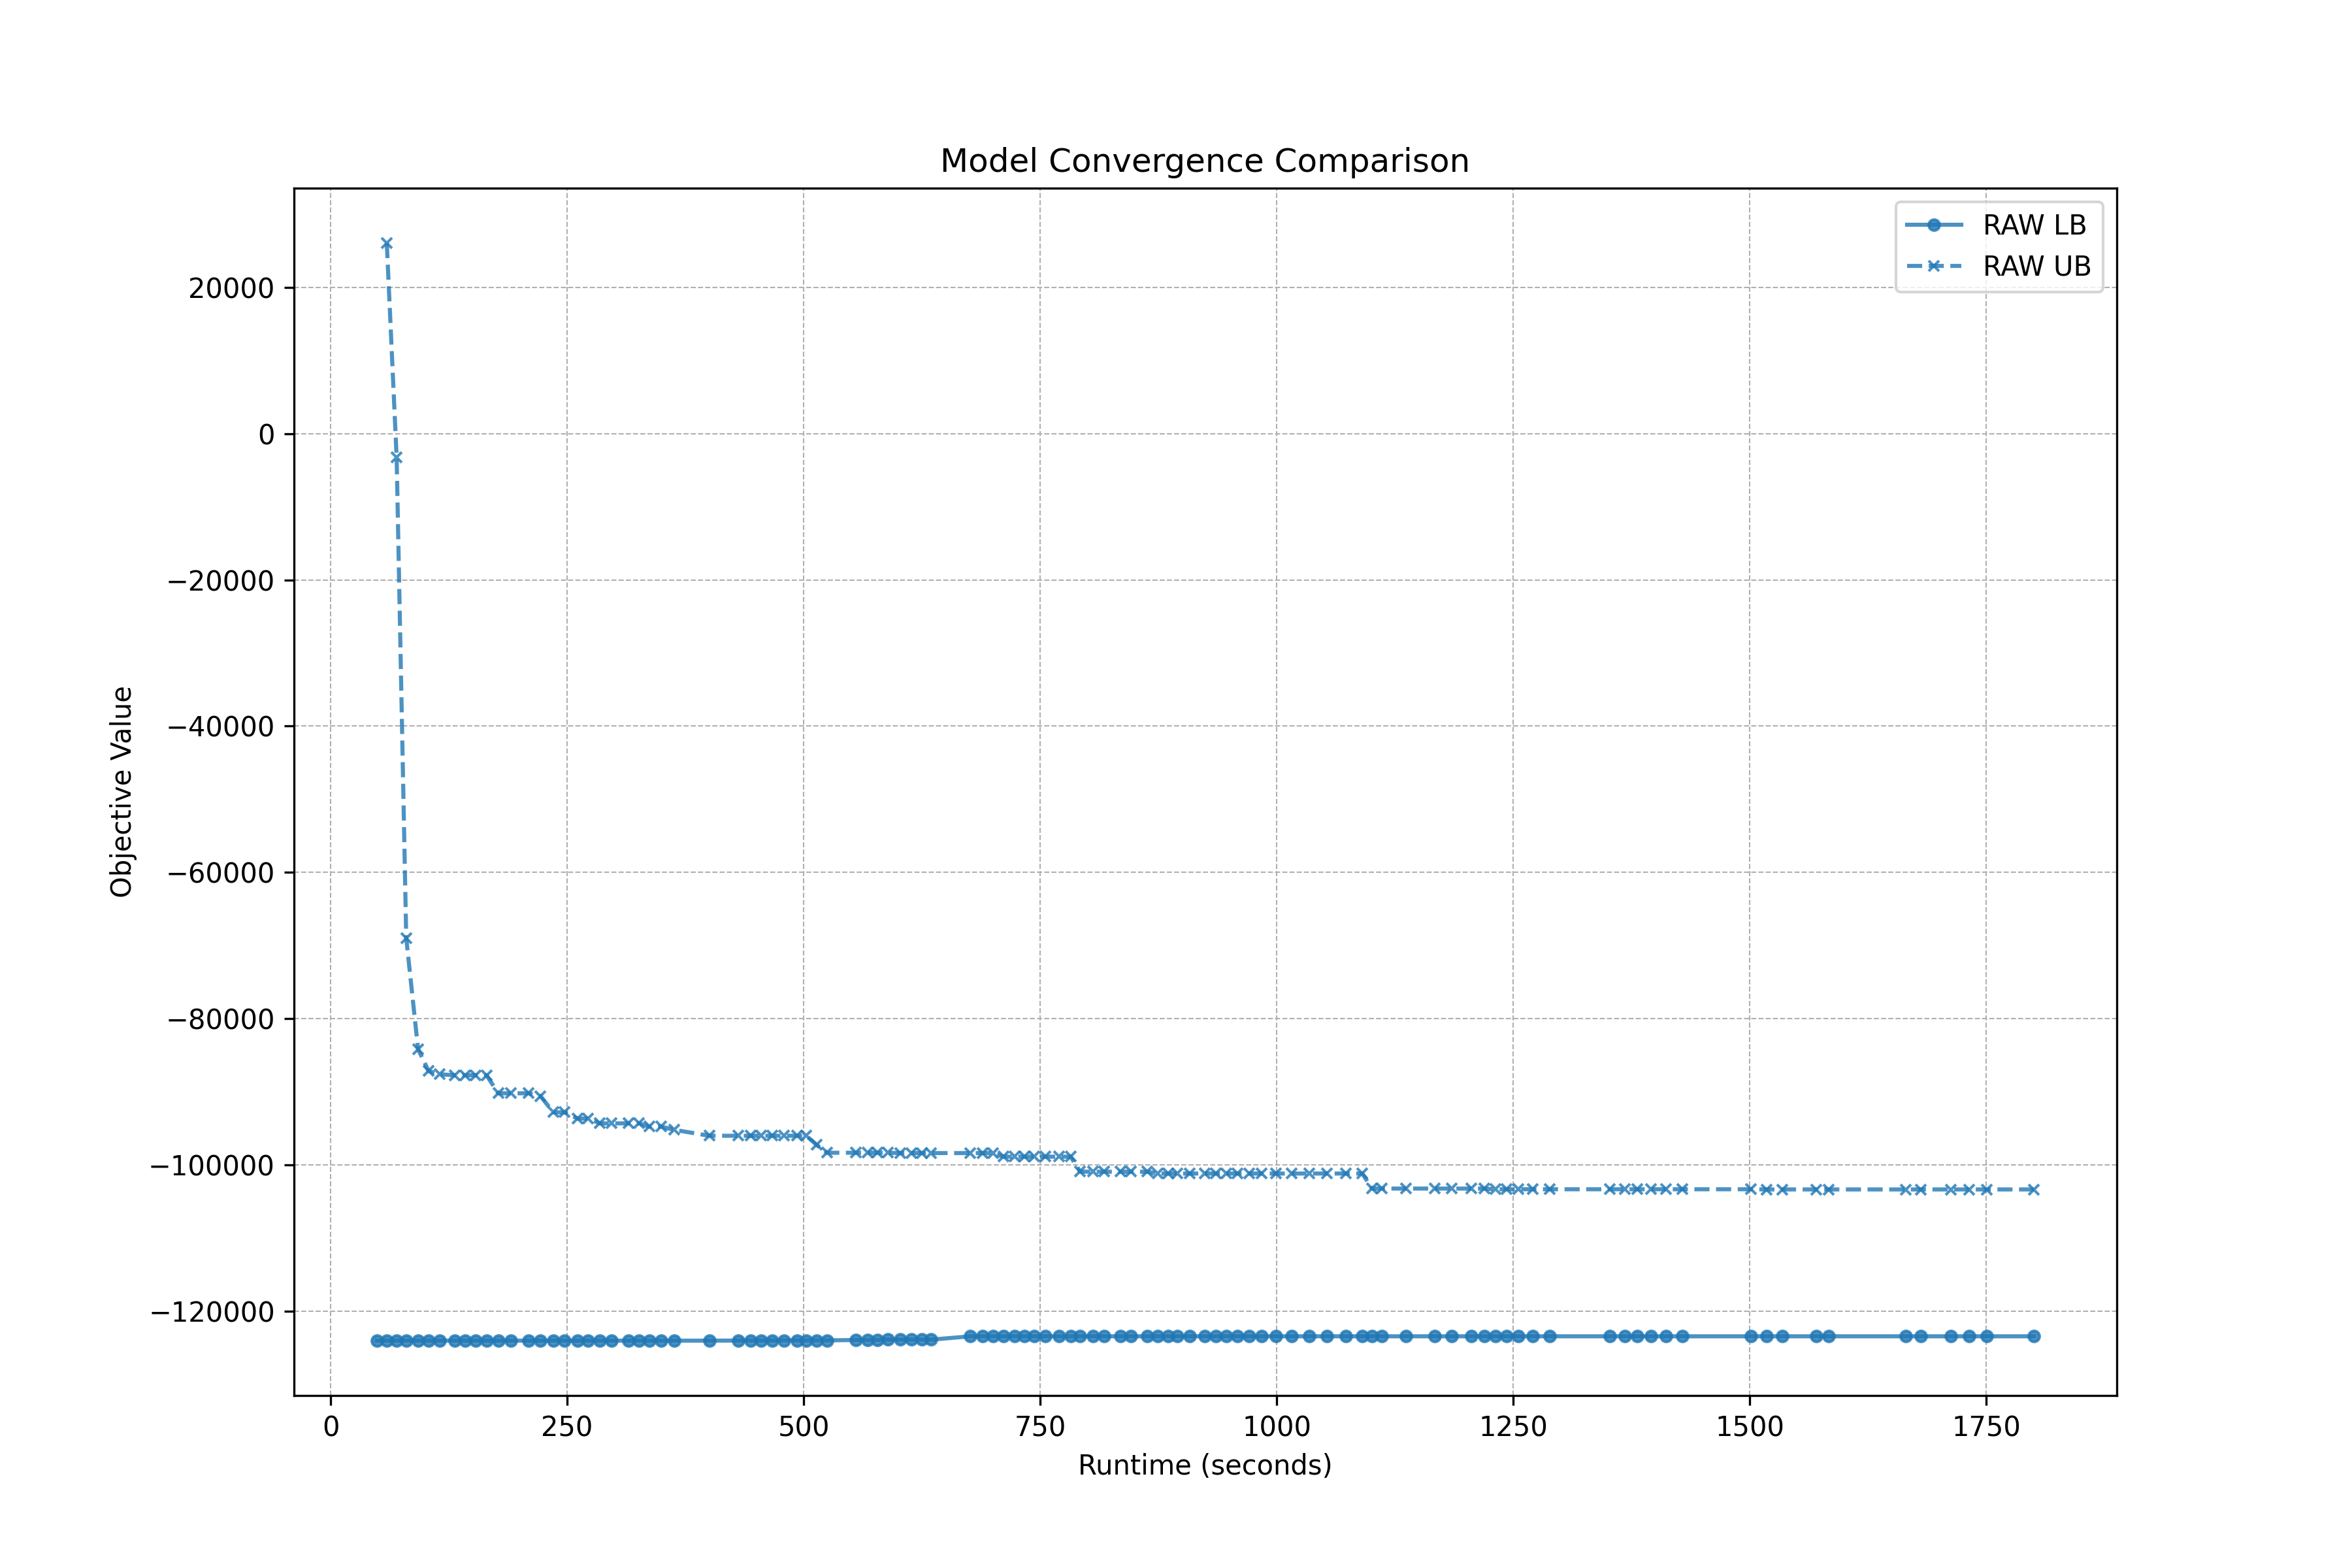
\includegraphics[width=0.8\textwidth]{figure/img/converge_f9_raw.png}
% %     \caption{Convergence Plot for F9, RAW}
% %     \label{fig:converge.f9.raw}
% % \end{figure}
% % \begin{figure}[h]
% %     \centering
% %     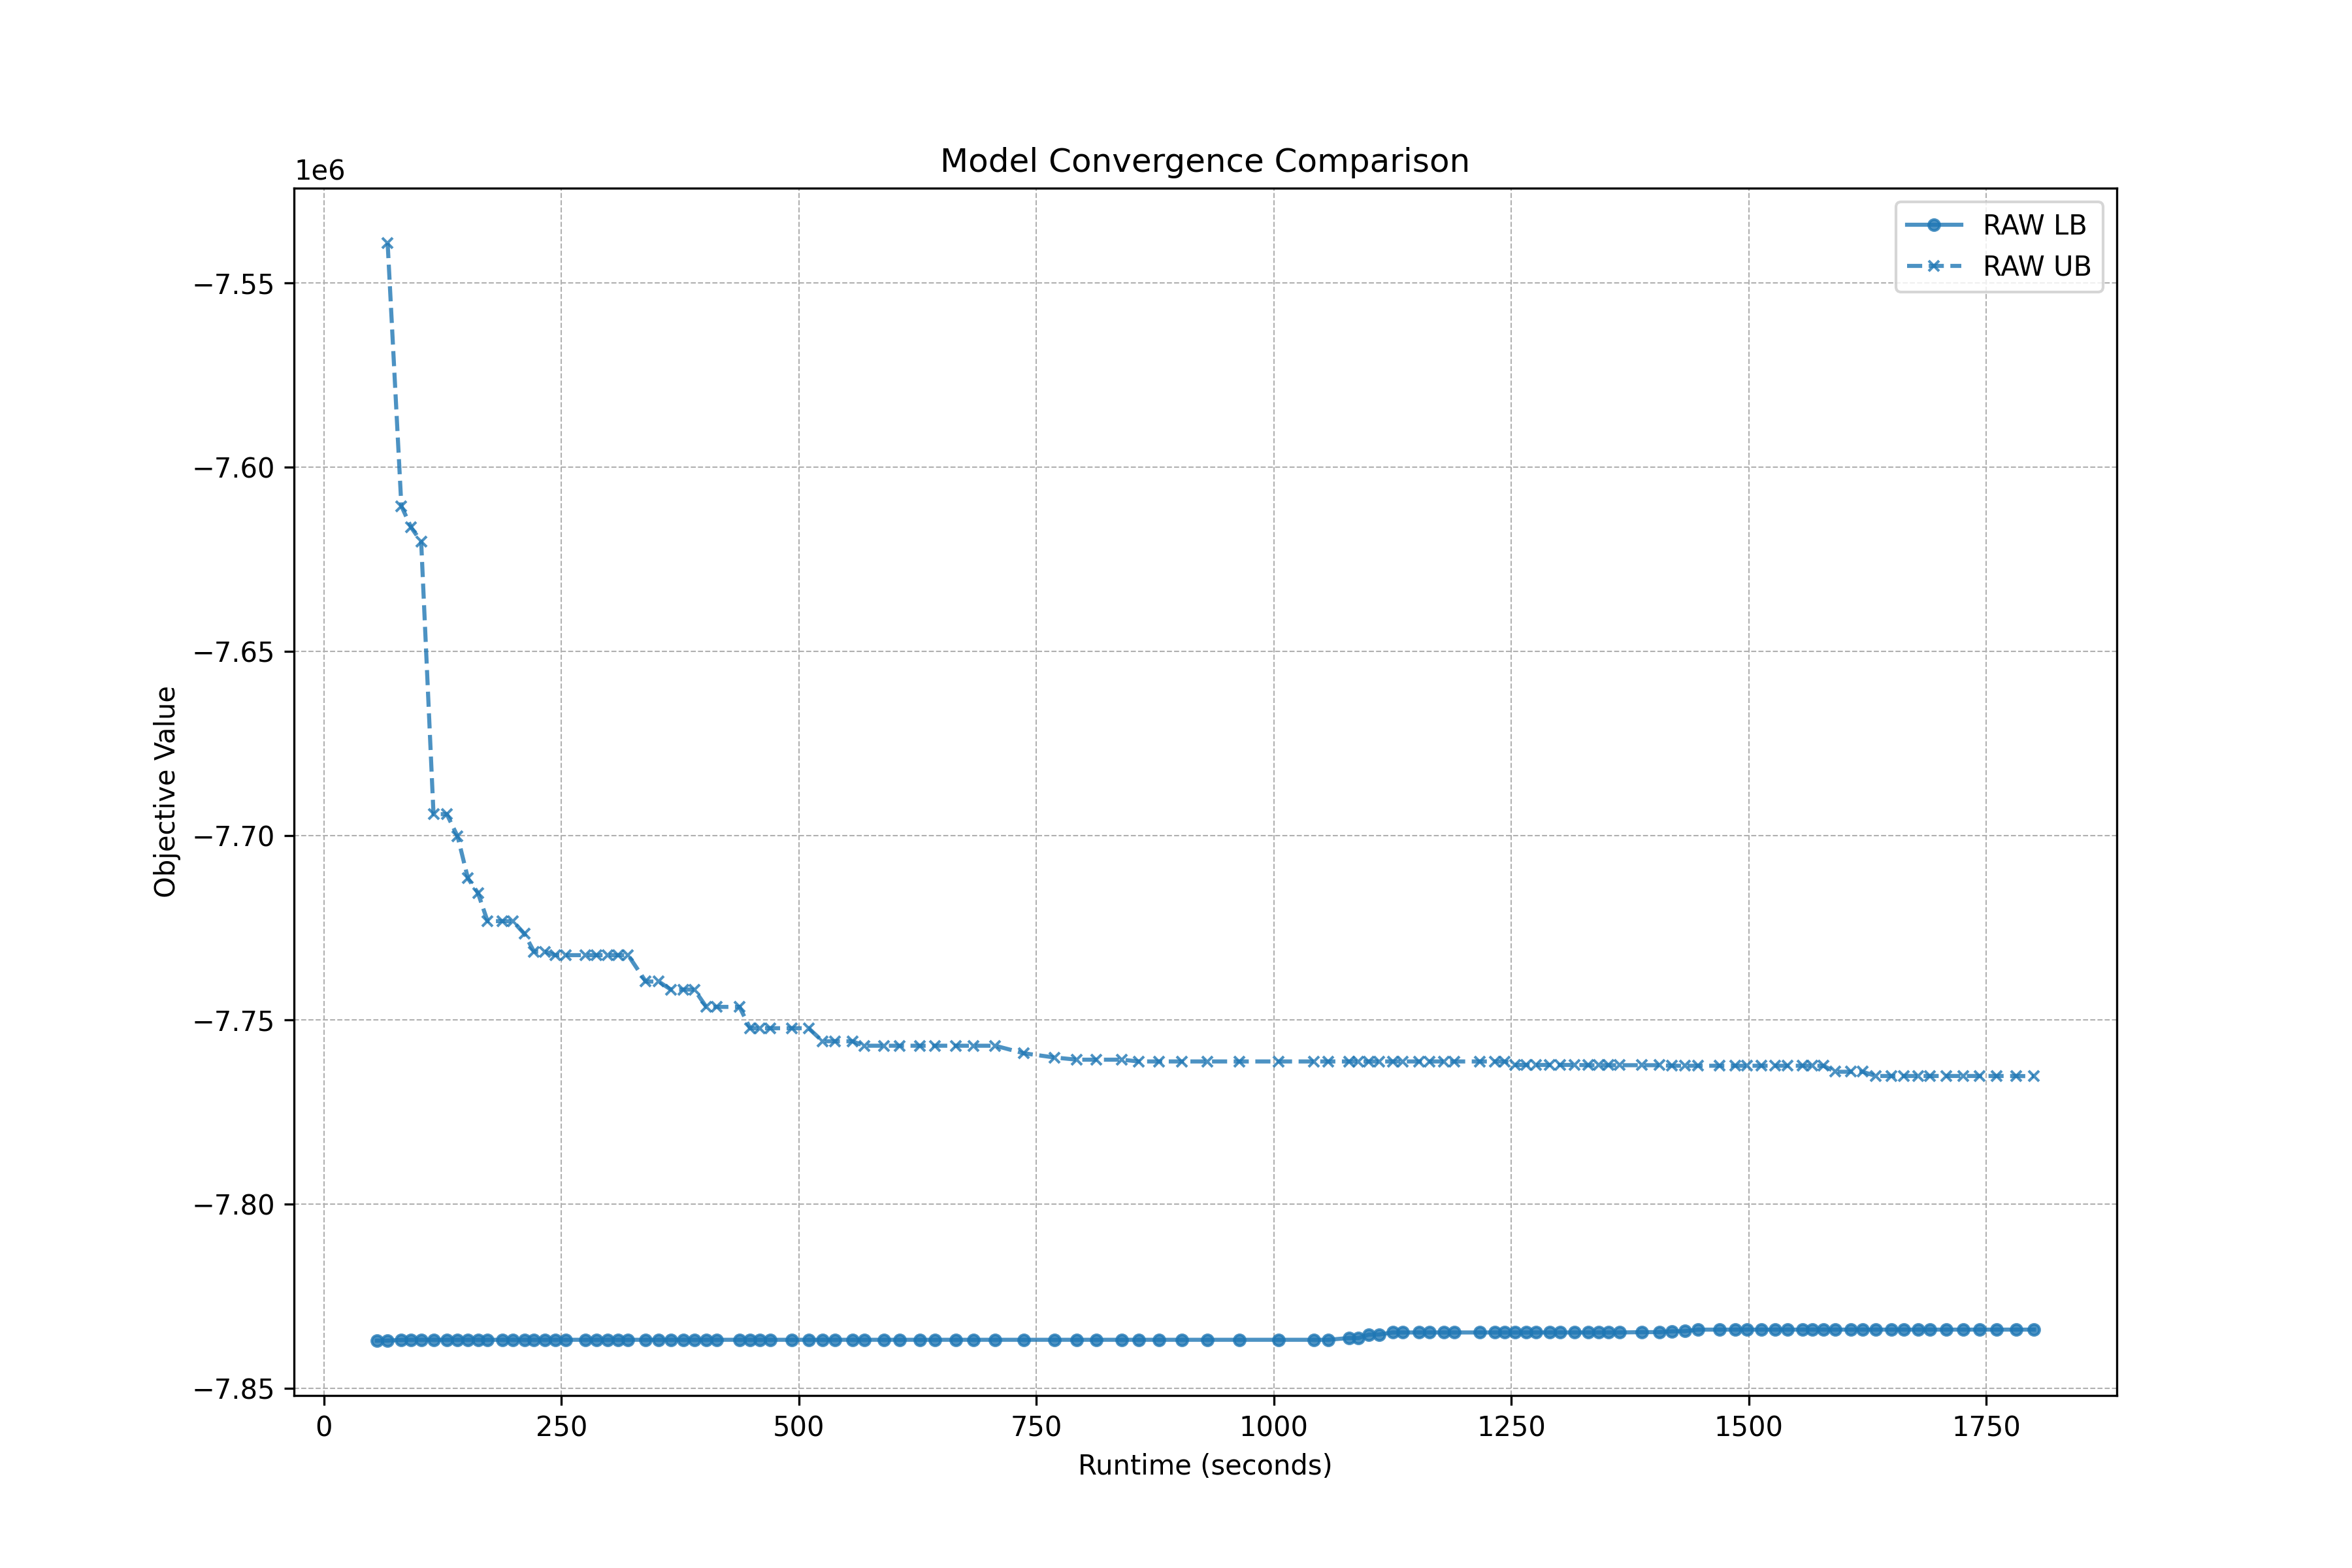
\includegraphics[width=0.8\textwidth]{figure/img/converge_b6_raw.png}
% %     \caption{Convergence Plot for B6, RAW}
% %     \label{fig:converge.b6.raw}
% % \end{figure}
% % \begin{figure}[h]
% %     \centering
% %     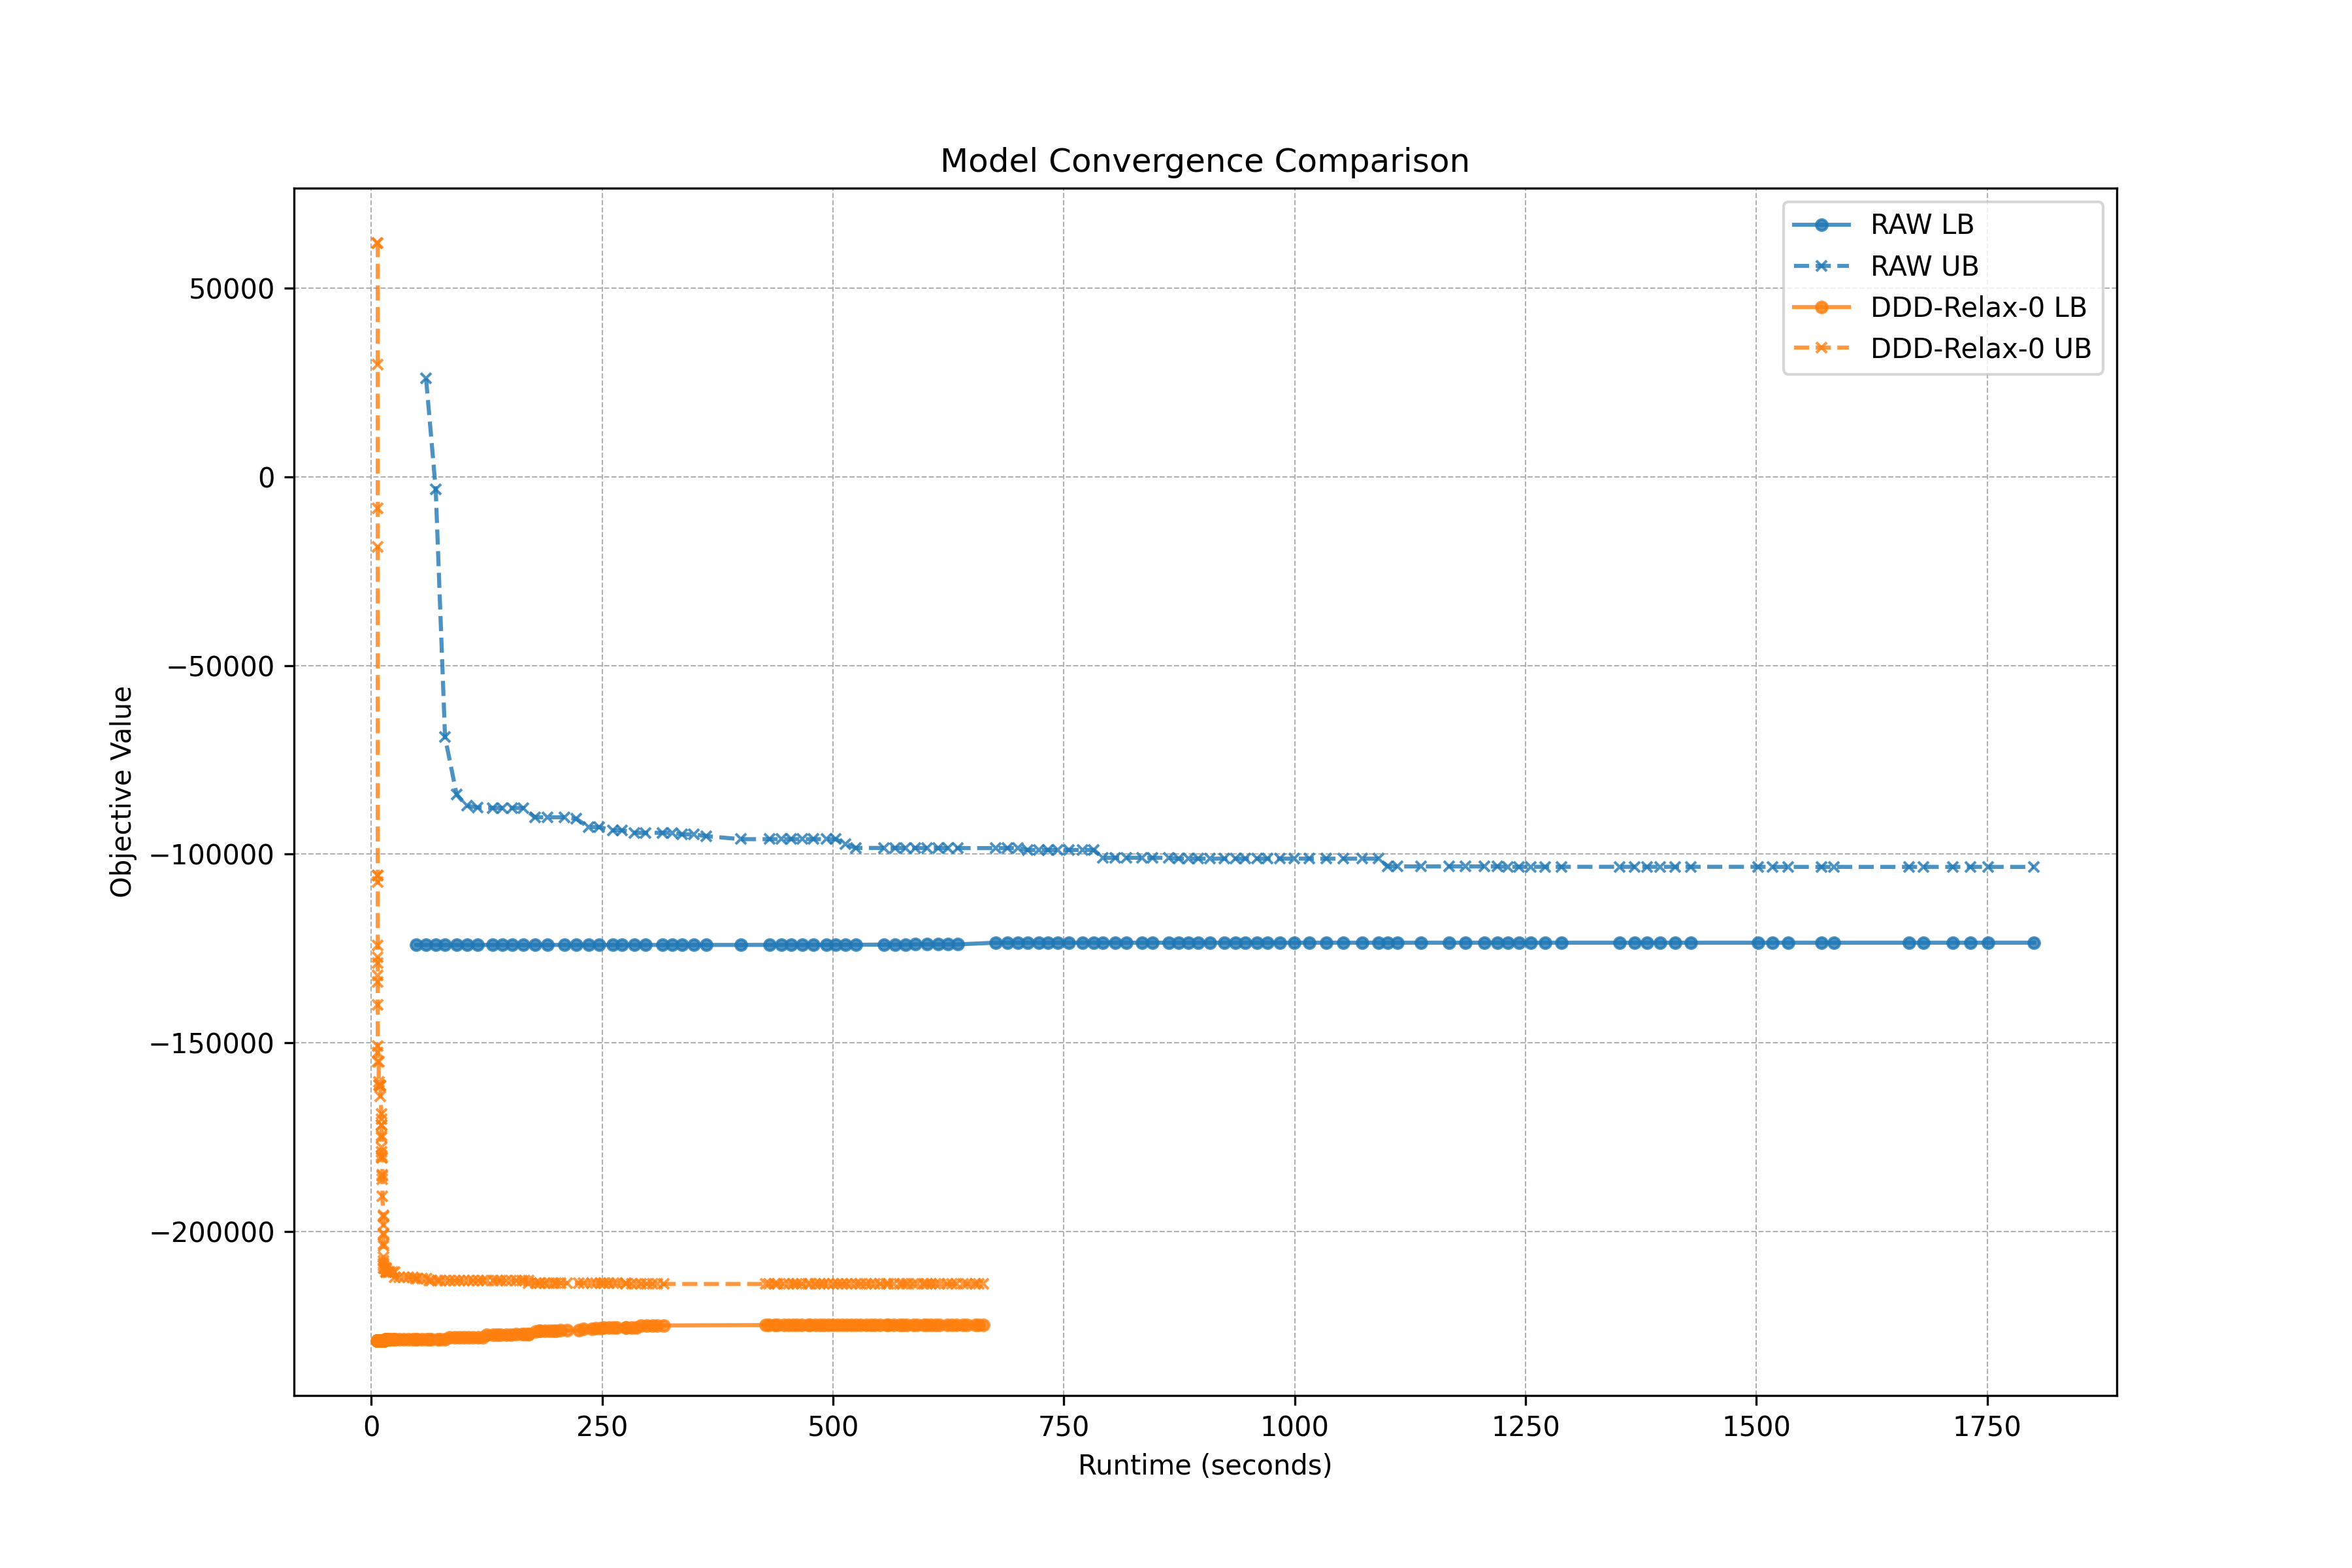
\includegraphics[width=0.8\textwidth]{figure/img/converge_f9_ddd_relax_0.png}
% %     \caption{Convergence Plot for F9, DDD-Relax, Method 0}
% %     \label{fig:converge.f9.ddd.r0}
% % \end{figure}
% % \begin{figure}[h]
% %     \centering
% %     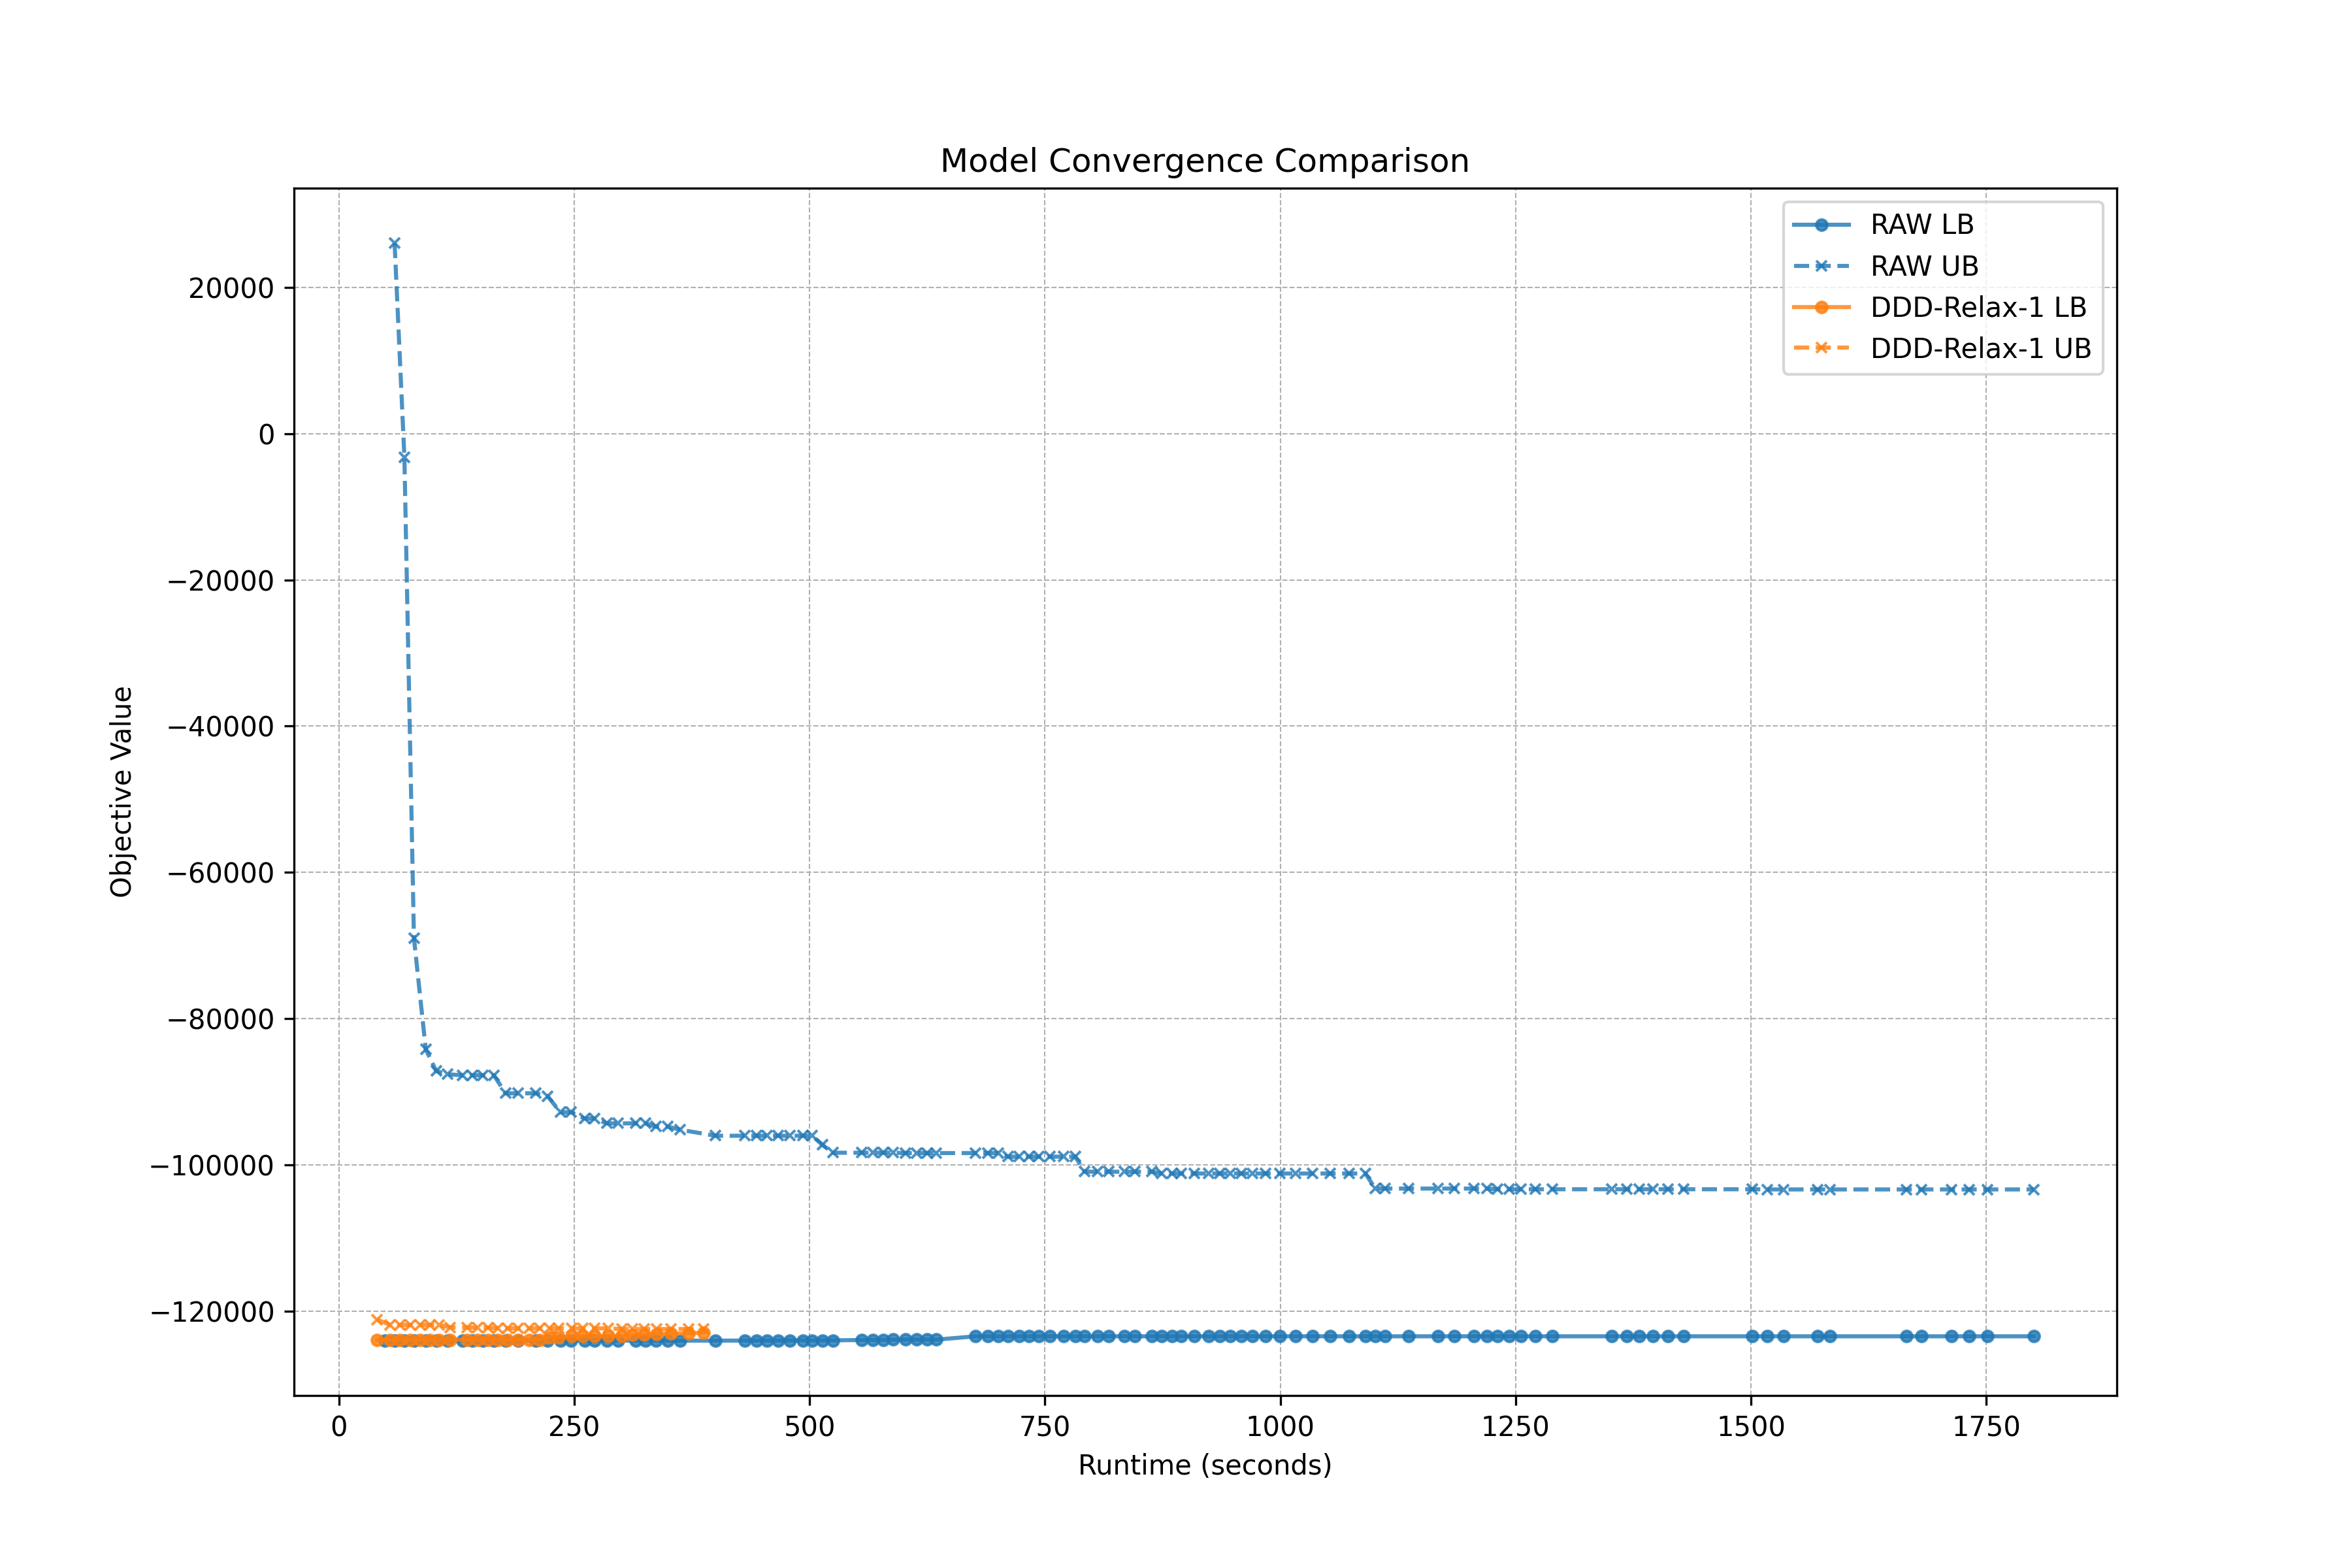
\includegraphics[width=0.8\textwidth]{figure/img/converge_f9_ddd_relax_1.png}
% %     \caption{Convergence Plot for F9, DDD-Relax, Method 1}
% %     \label{fig:converge.f9.ddd.r1}
% % \end{figure}
% % \begin{figure}[h]
% %     \centering
% %     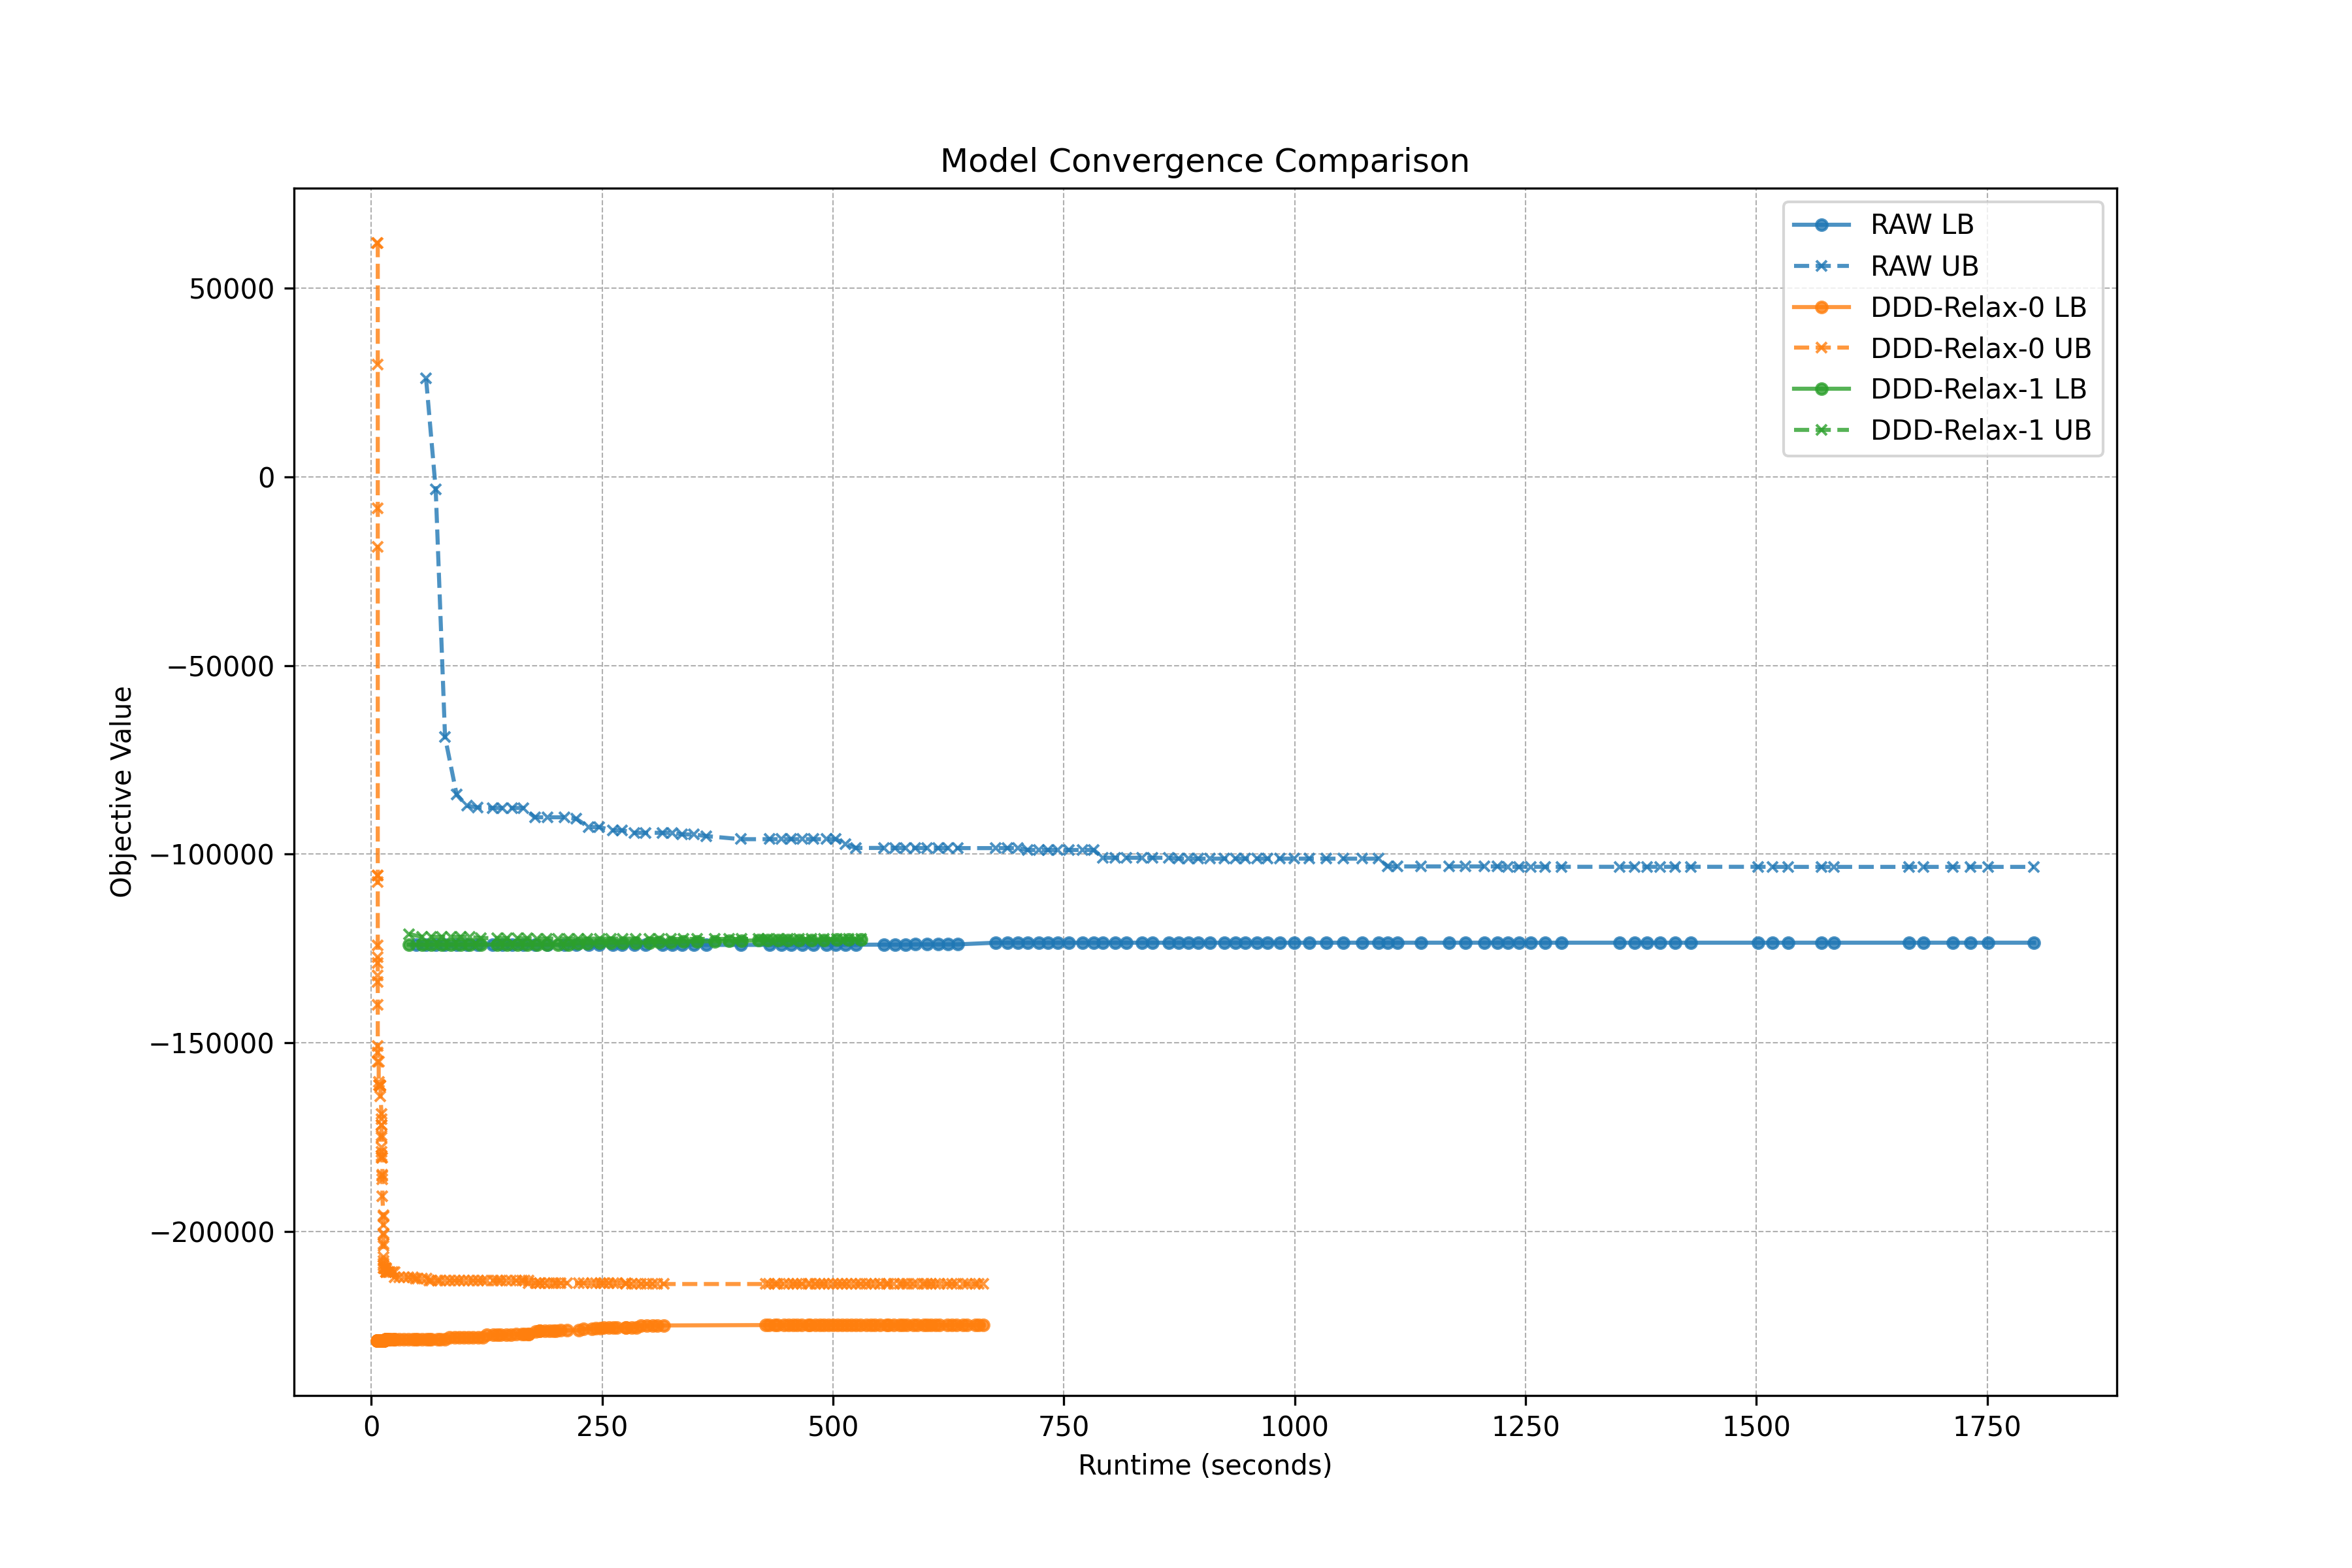
\includegraphics[width=0.8\textwidth]{figure/img/converge_f9_ddd_relax_01.png}
% %     \caption{Convergence Plot for F9, DDD-Relax, Method 0\&1}
% %     \label{fig:converge.f9.ddd.r0r1}
% % \end{figure}
% % \begin{figure}[h]
% %     \centering
% %     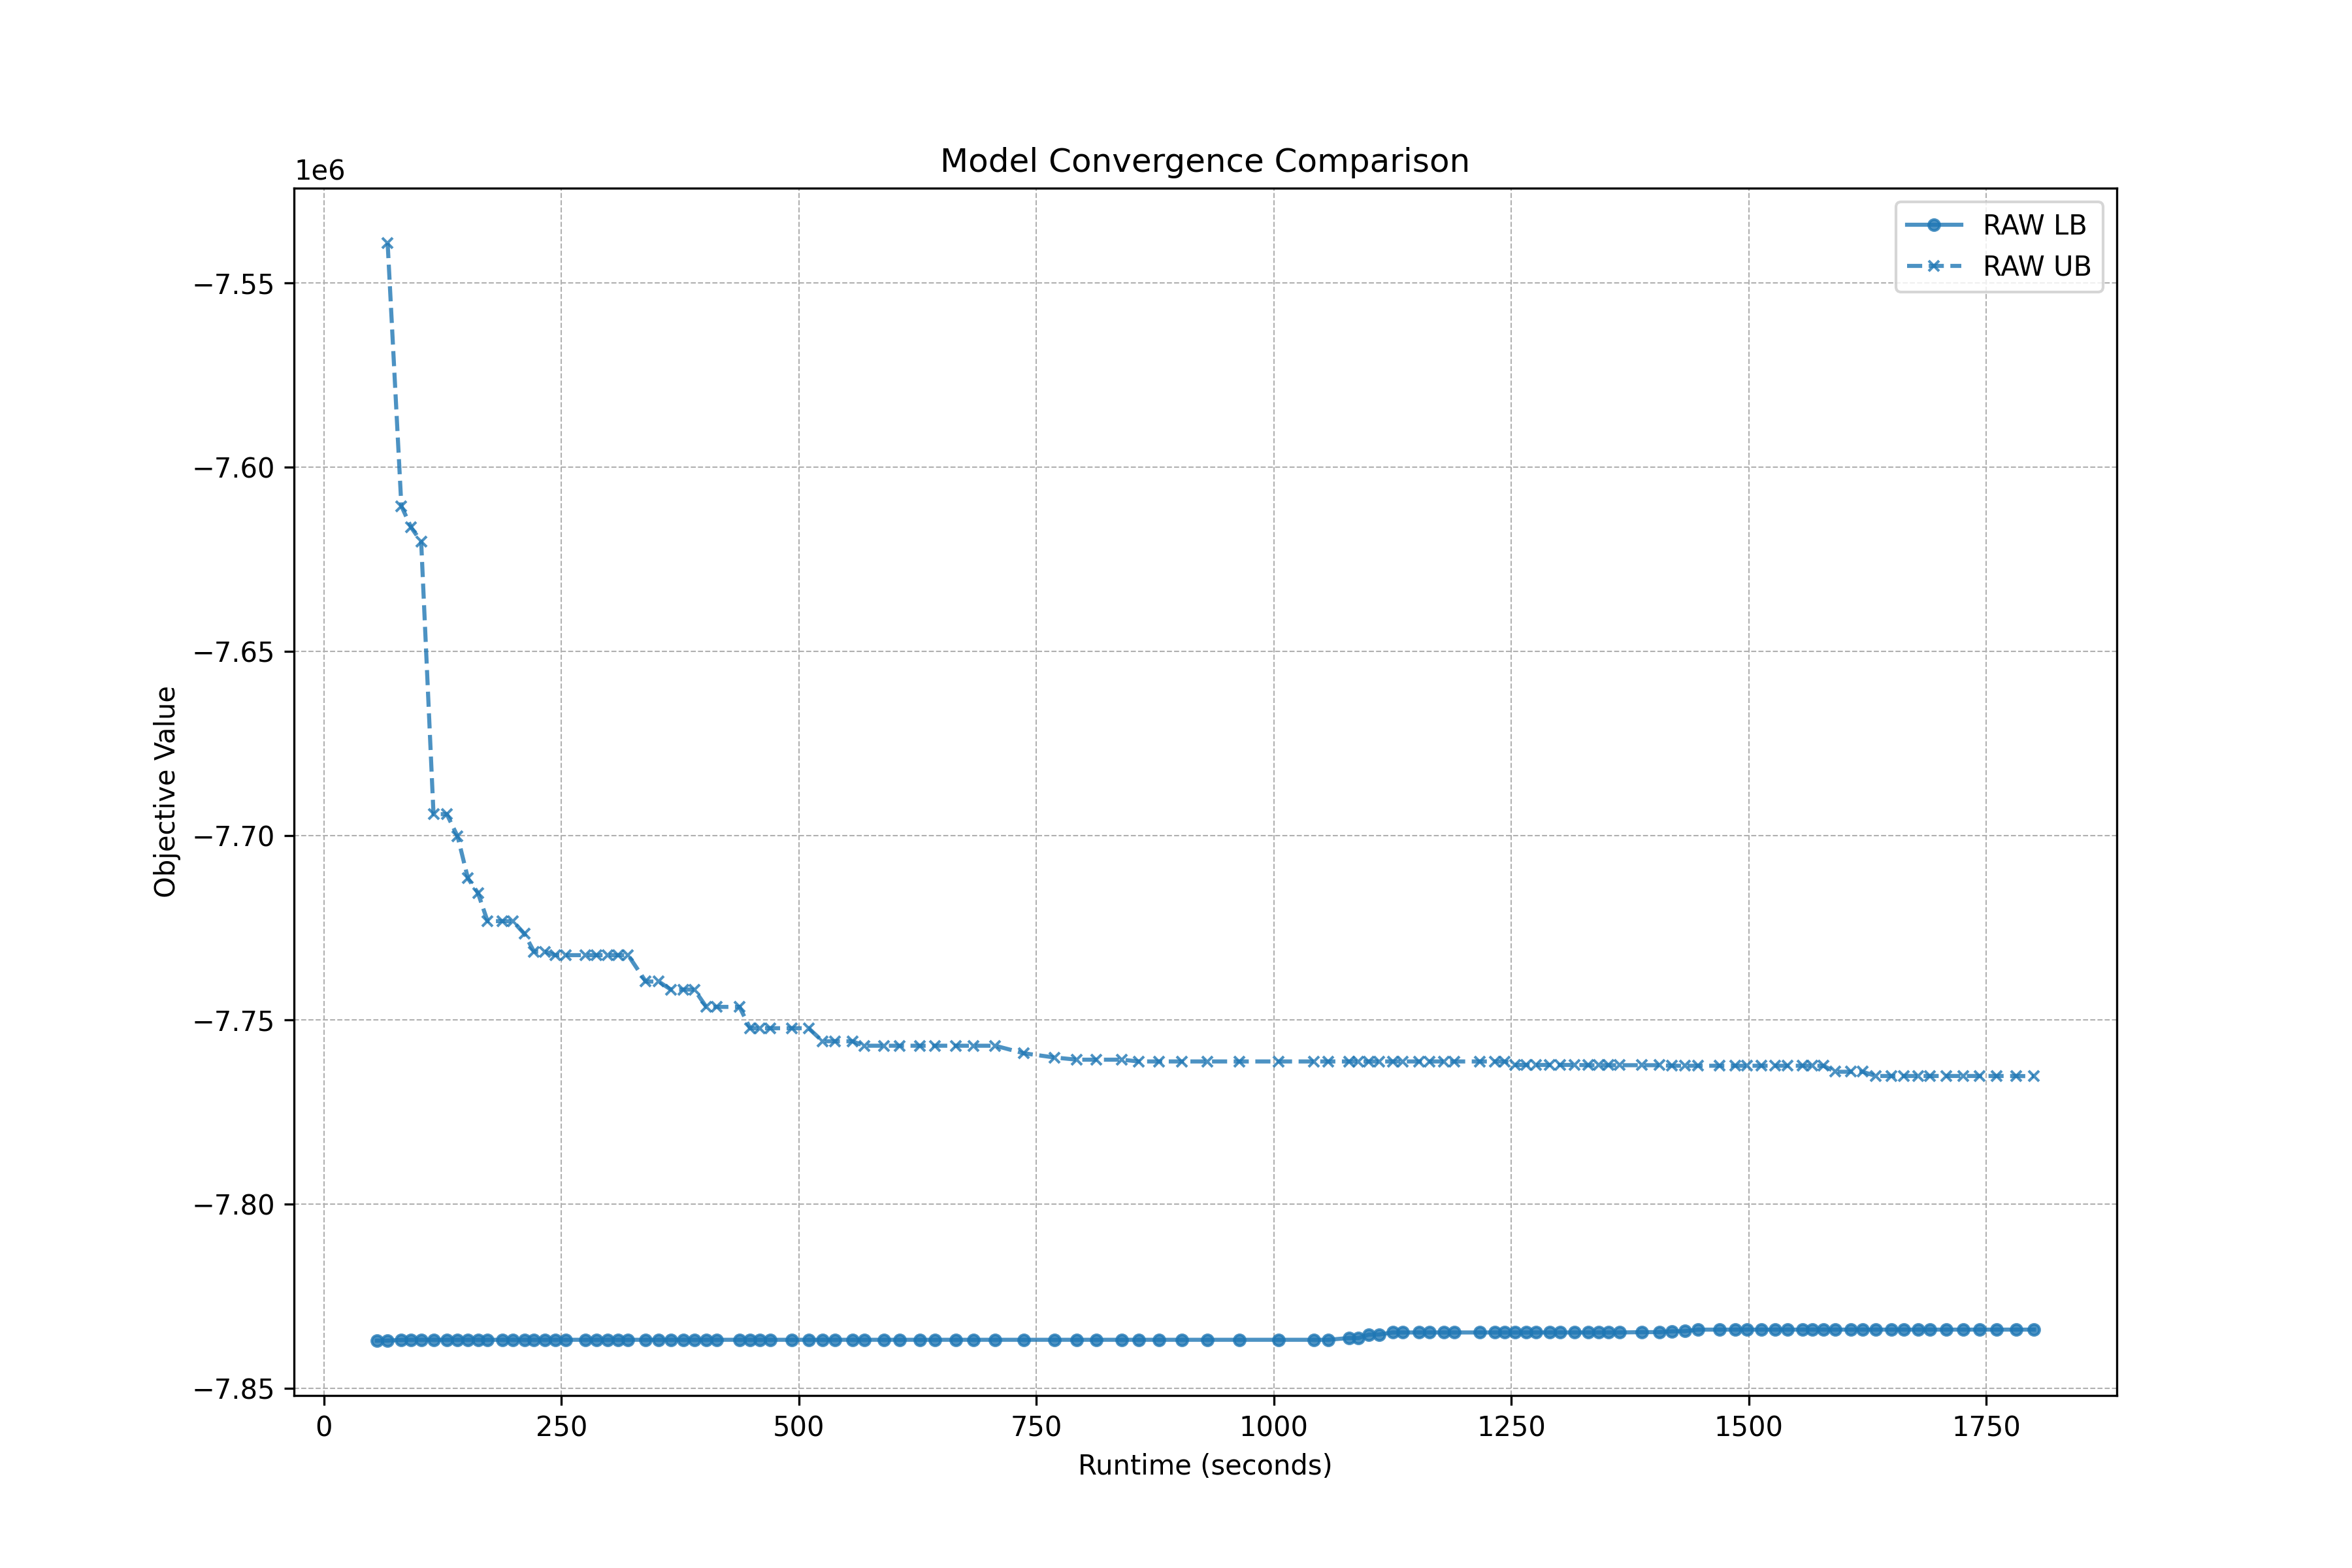
\includegraphics[width=0.8\textwidth]{figure/img/converge_b6_raw.png}
% %     \caption{Convergence Plot for B6, RAW}
% %     \label{fig:converge.b6.raw}
% % \end{figure}
% % \subsection{FDM and Upper Bound}
% % \subsection{Refine Strategy}

% \begin{figure}[ht]
%   \centering
%   \begin{subfigure}{0.48\textwidth}
%     \centering
%     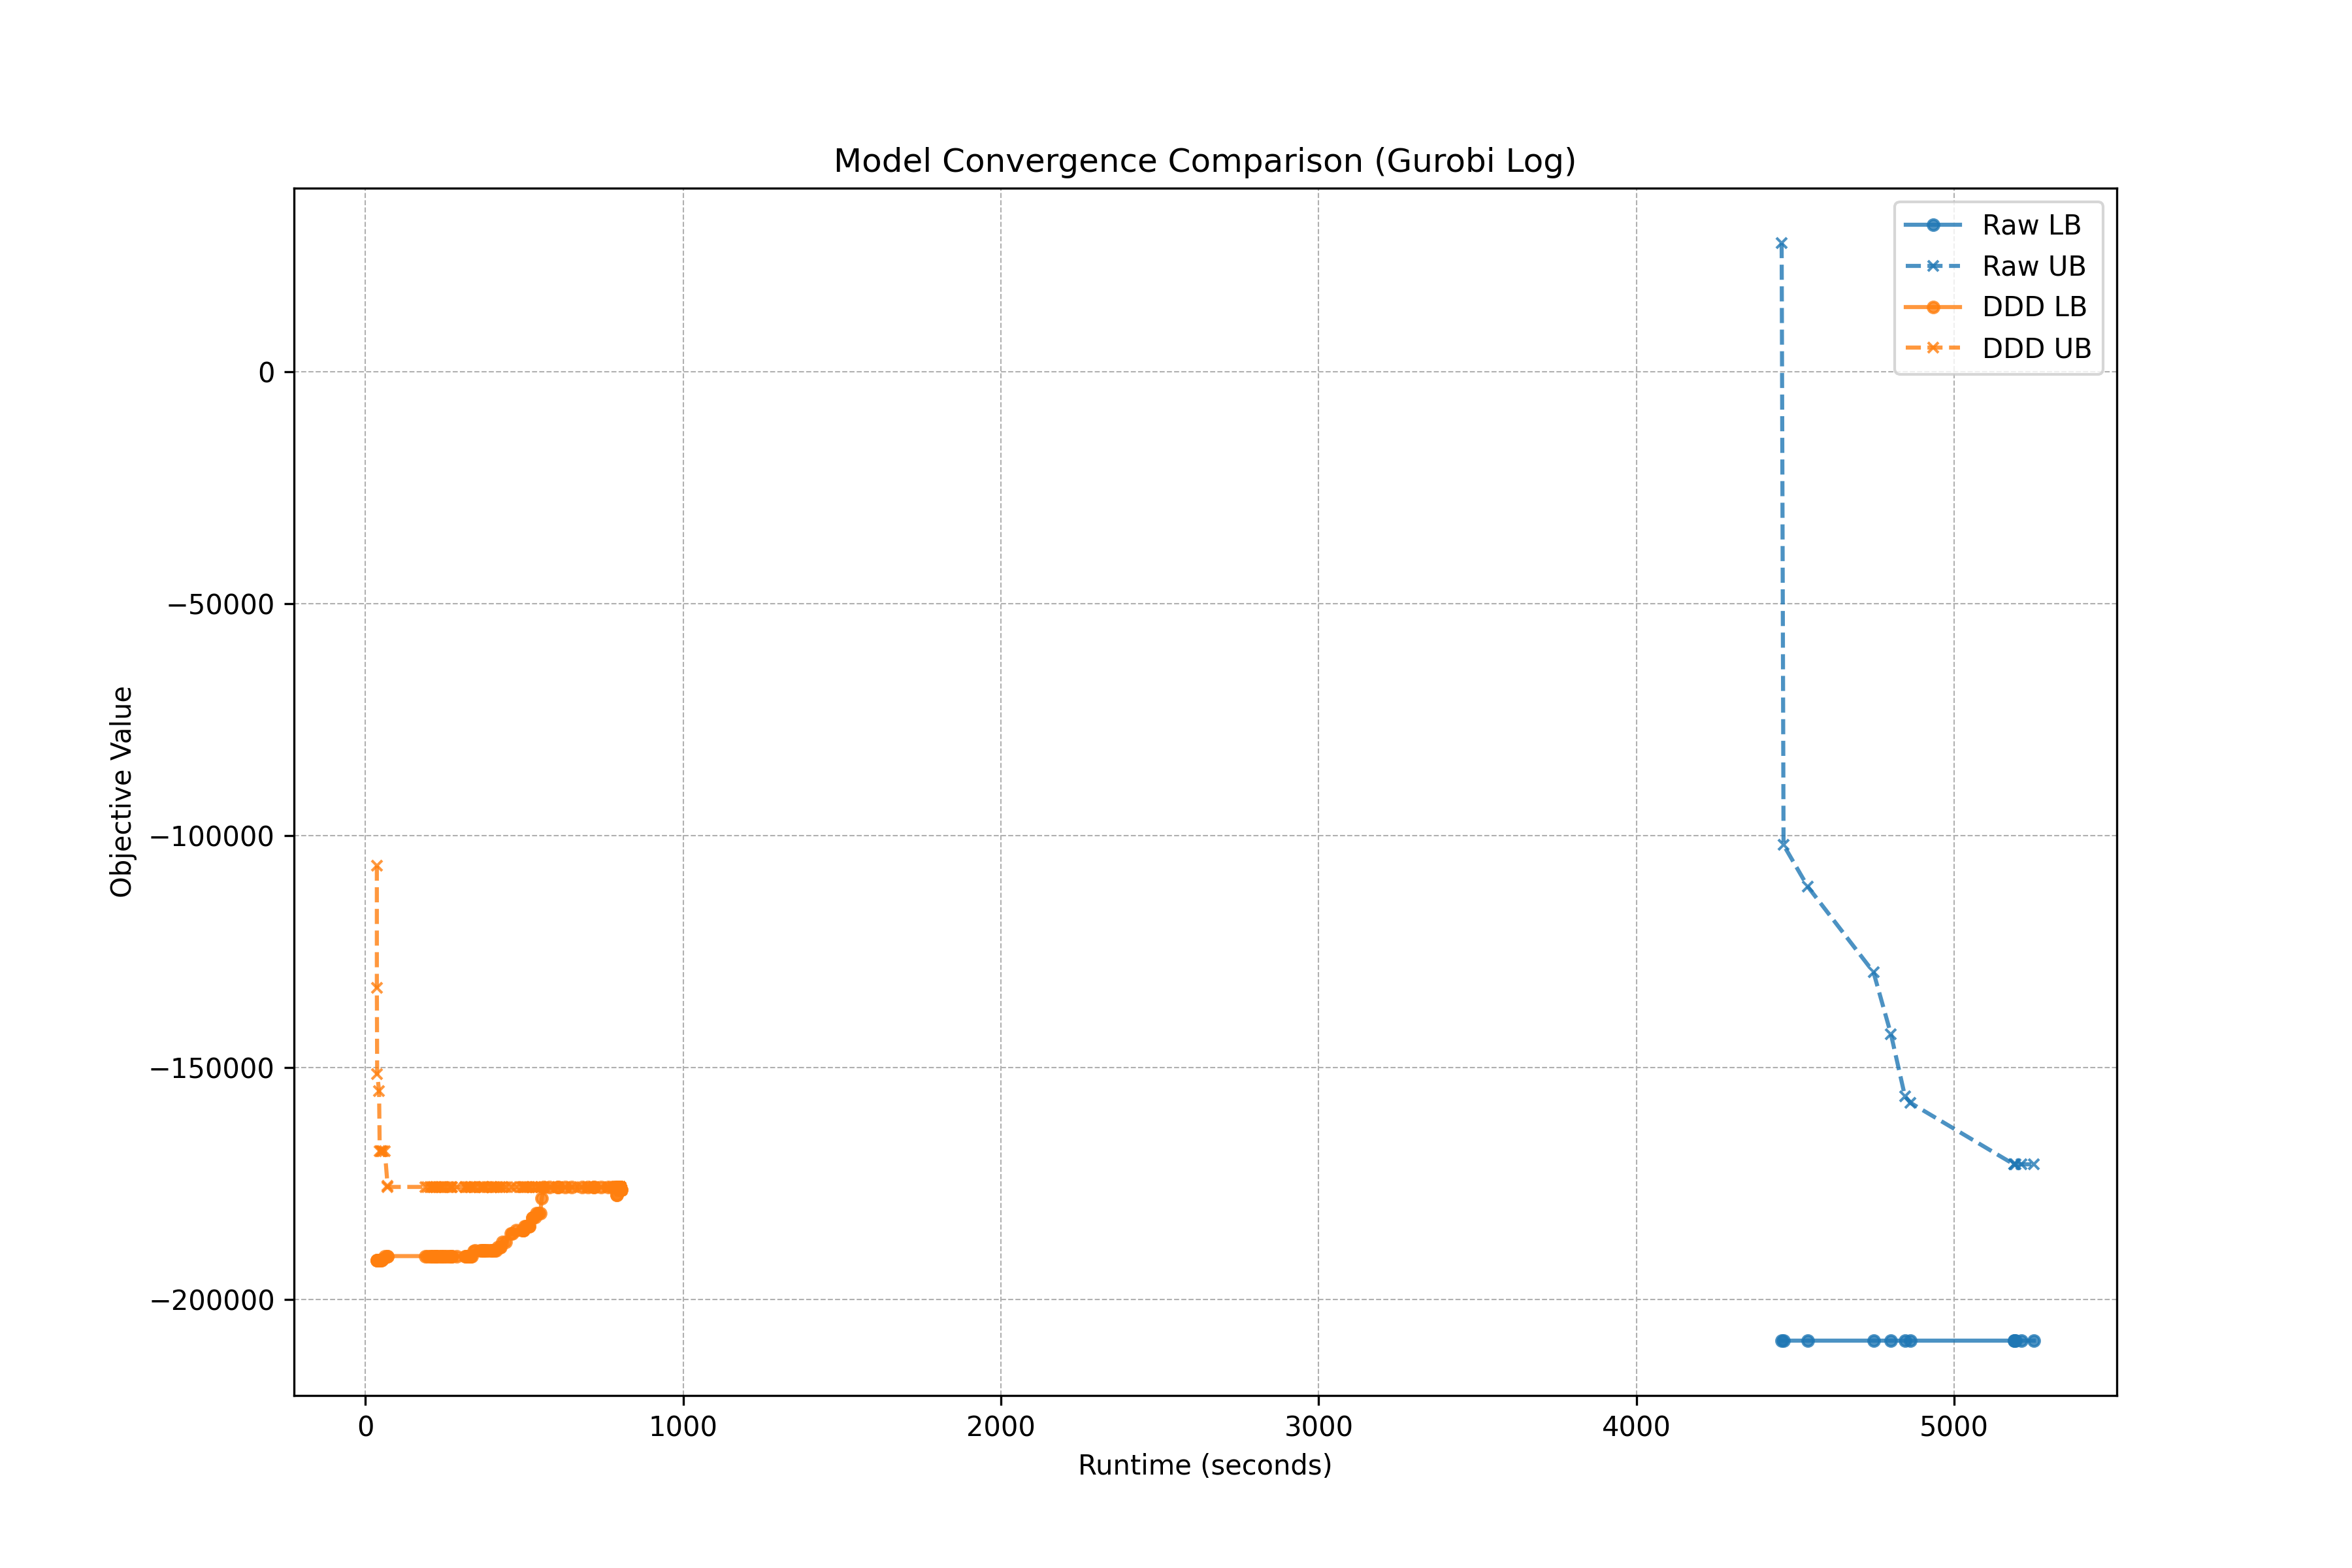
\includegraphics[width=\textwidth]{figure/img/converge_f9_nddd.png}
%     \caption{RAW vs DDD}
%     \label{fig:converge.f9.nddd}
%   \end{subfigure}
%   \hfill
%   \begin{subfigure}{0.48\textwidth}
%     \centering
%     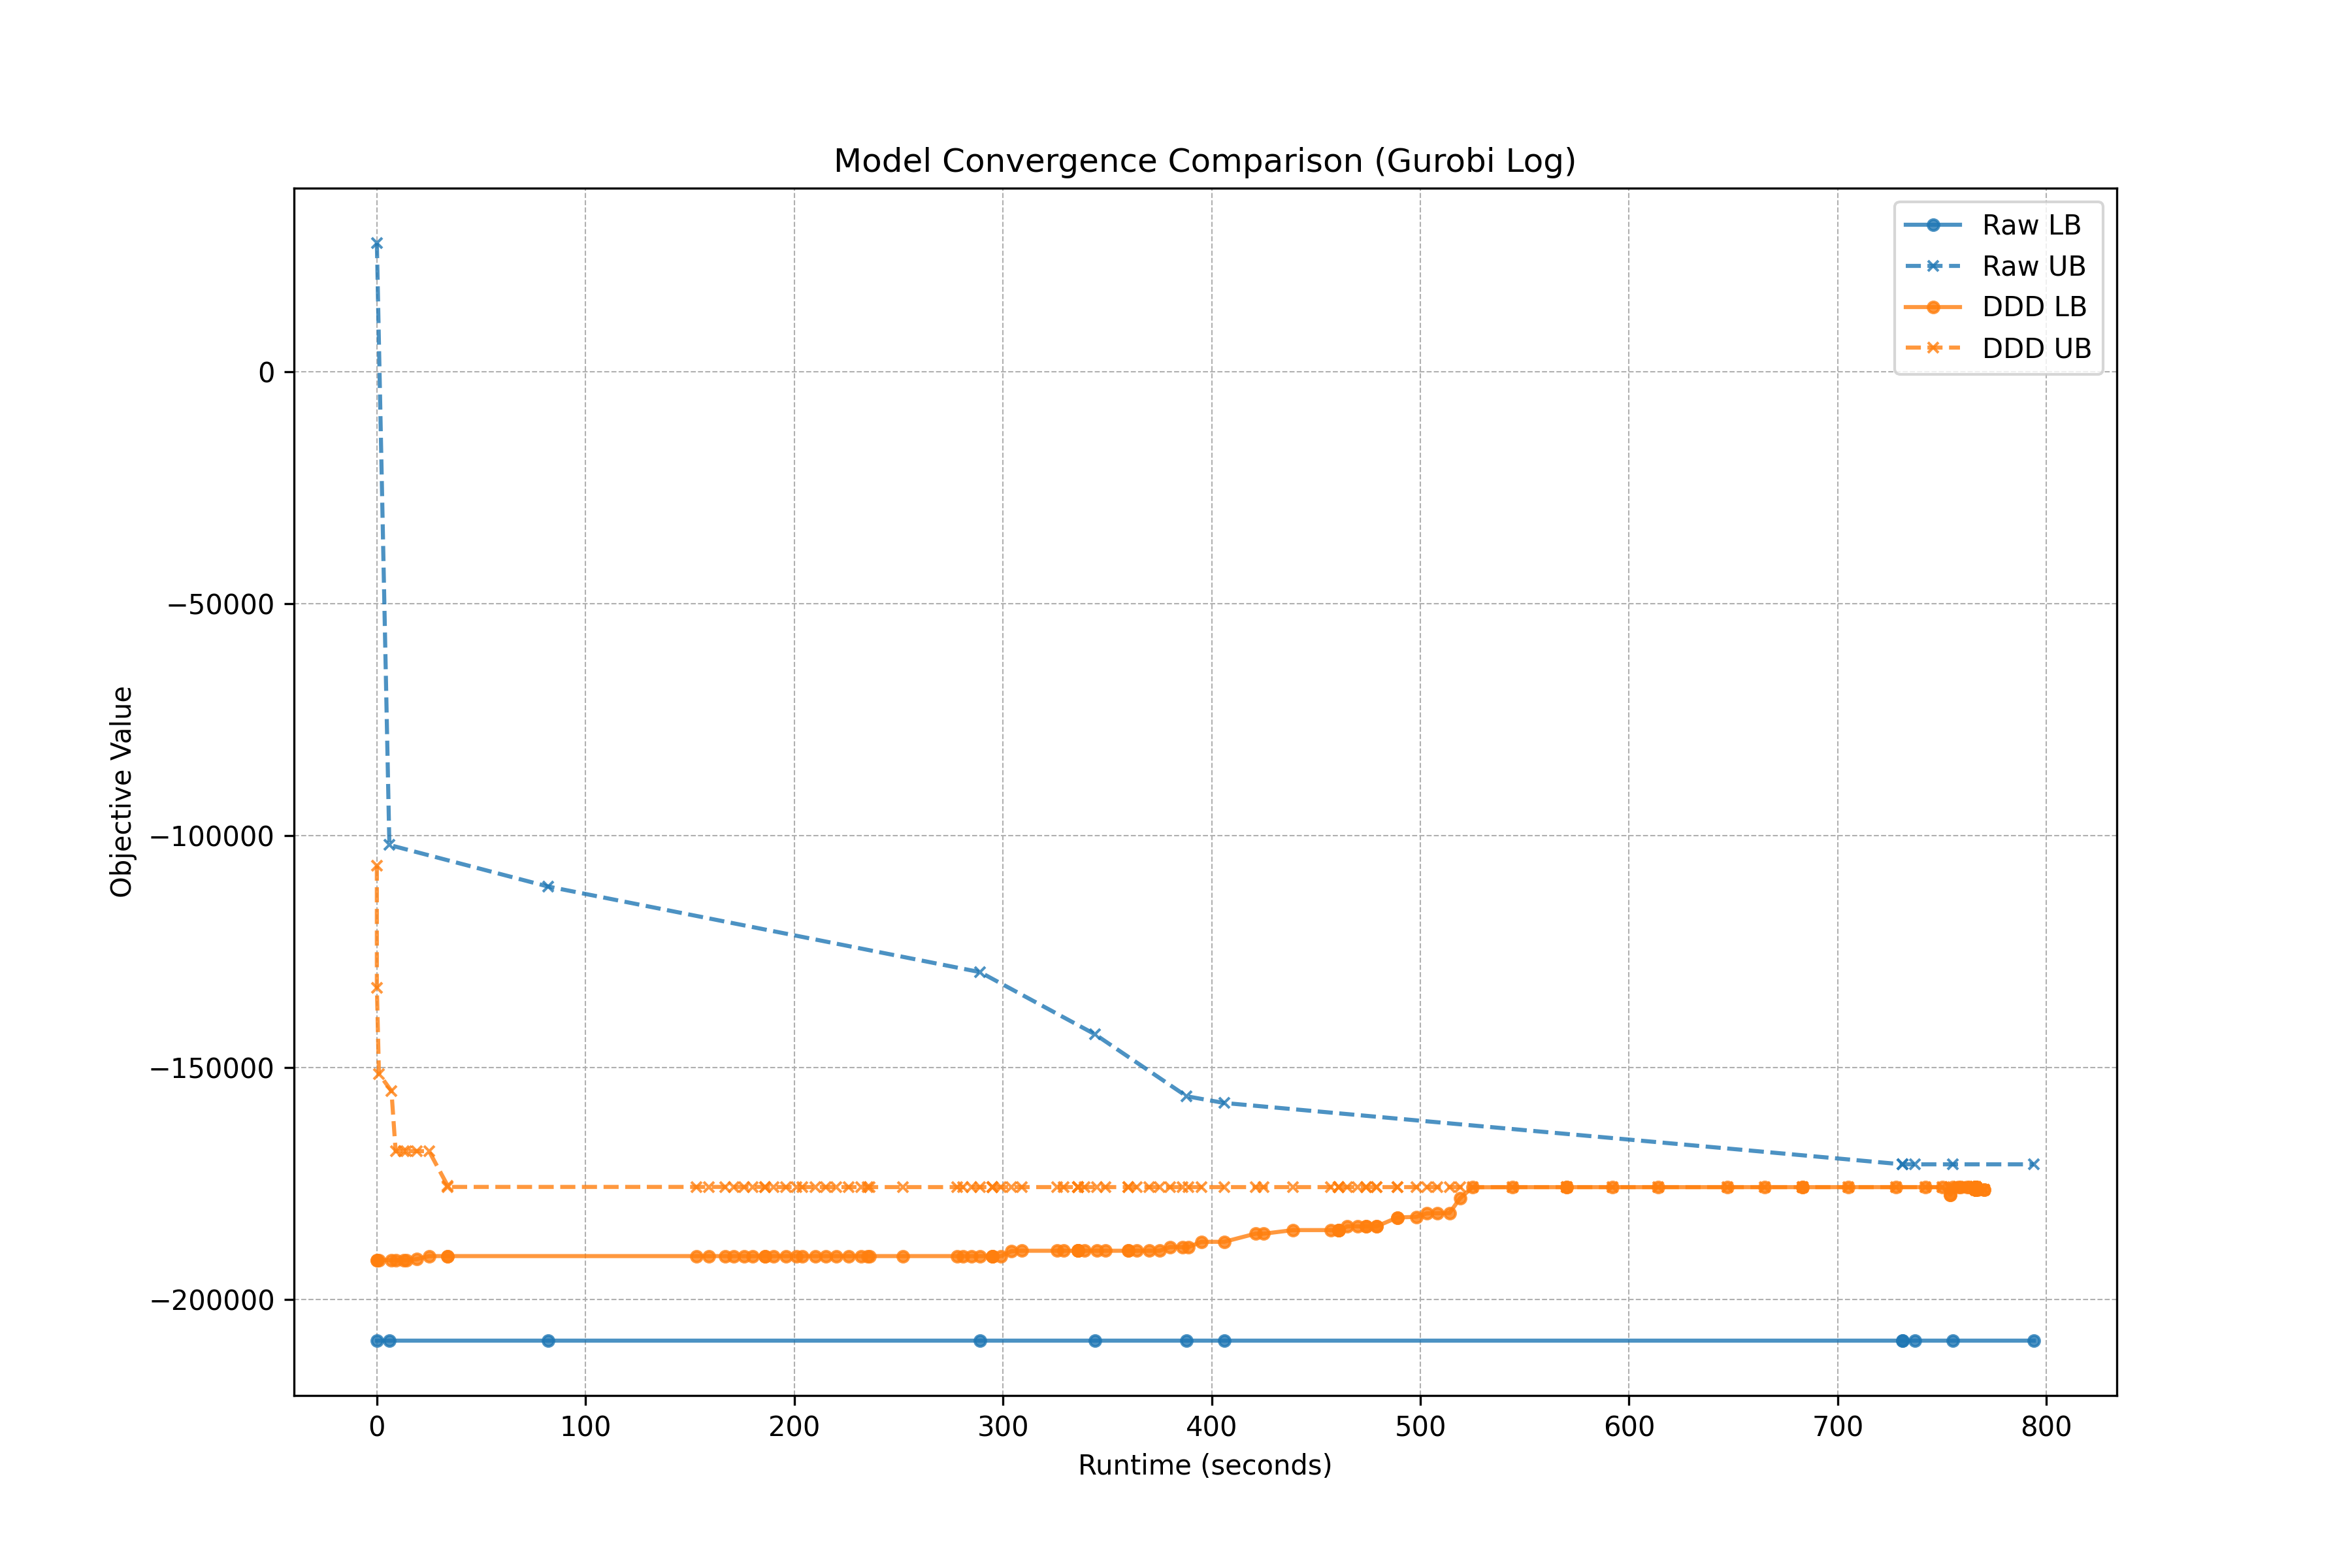
\includegraphics[width=\textwidth]{figure/img/converge_f9_nddd_aligned.png}
%     \caption{RAW vs DDD (Aligned)}
%     \label{fig:converge.f9.nddd.aligned}
%   \end{subfigure}
%   \caption{Convergence Plot for F9}
% \end{figure}

% Table \ref{tab:results_comparison} presents the computational solutions for the selected instance, comparing the performance of DDD against standard benchmarks. The proposed DDD framework (specifically the IDDD implementation) demonstrates superior performance. IDDD achieves the highest profit of \$176,403 with a remarkably tight global optimality gap of 0.24\%.This is achieved by effectively combining the strong lower bound from the relaxed model (IDDD-Relax, \$176,829) and the high-quality integer solution from the Vantage algorithm (IDDD-UB). In comparison, the direct implementation using the commercial solver Gurobi struggles to converge, yielding a significant 22.25\% gap and a lower profit (\$170,883) even after 5 hours of computation on a high-memory machine. The Multi-Phase decomposition method, while reporting a 0.00\% gap, converged to a significantly inferior local optimum (\$64,367), verifying that it fails to effectively explore the full search space. Thus, DDD provides the best computational efficiency (0.78 hours), and proof of optimality. 

% \begin{table}
% \caption{Comparison to Benchmarks\label{tab:results_comparison}}
% \centering
% \begin{tabular}{l c c c c}
% \toprule
% \textbf{Method} & \textbf{\% Gap} & \textbf{Profit (\$)} & \textbf{CPU (hr)} & \textbf{Status} \\
% \midrule
% \multirow{2}{*}{Gurobi Directly}
% & N/A & N/A & 0.67 & TL \\
% & 22.25 & 170,883.04 & 5.00 & SU \\
% [0.5em]
% \multirow{2}{*}{DDD} & N/A & N/A & 0.67 & TL \\
% & N/A & N/A & 5.00 & TL \\
% [0.5em]
% \multirow{2}{*}{Multi-Phase}
% & 17.3 & 64,336.39 & 0.67 & SU\\
% & 0.00 & 64,367.08 & 5.00 & C-SU\\
% [0.5em]
% \multirow{1}{*}{IDDD-Relax} & 0.00 & 176,829.19 & 0.11 & C-RE \\
% \multirow{1}{*}{IDDD-UB{\tiny (VANTAGE)}} & 0.00 & 176,403.40 & 0.67 & C-SU \\
% \multirow{1}{*}{IDDD} & 0.24 & 176,403.40 & 0.78 & C \\
% \bottomrule
% \end{tabular}

% {\tiny
% TL: Too long to find a solution;
% OOM: Out of memory error;
% SU: Suboptimal;
% RE: Relaxed;
% C: Converged.
% }
% \end{table}

% \begin{table}[htbp]
% \caption{Detailed Results for Solution (IDDD Case)}
% \centering
% \scriptsize
% \setlength{\tabcolsep}{2pt}
% \begin{tabular}{llrrrrrrrrr}
% \toprule
% Airline & Method & Type & Seg & Flt & Pax & Seat & Cost & Rev & PPF & LF \\
% \midrule
% \multirow{10}{*}{F9} 
% & \multirow{5}{*}{\shortstack[l]{RAW\\Obj: 175,519.34\\Gap: 19.02\%}}
% & H2H & 122 & 172 & 25,537.23 & 36,192 & 2,211,714.09 & 2,974,400.73 & 148.47 & 0.71 \\
% & & H2S & 52 & 86 & 4,920.27 & 17,112 & 1,307,002.48 & 578,732.87 & 57.21 & 0.29 \\
% & & S2H & 81 & 86 & 10,093.86 & 17,112 & 1,098,979.91 & 1,292,753.26 & 117.37 & 0.59 \\
% & & S2S & 4 & 4 & 0.00 & 768 & 52,671.04 & 0.00 & 0.00 & 0.00 \\
% & & \textbf{Total} & \textbf{259} & \textbf{348} & \textbf{40,551.36} & \textbf{71,184} & \textbf{4,670,367.52} & \textbf{4,845,886.86} & \textbf{116.53} & \textbf{0.57} \\
% \cmidrule{2-11}
% & \multirow{5}{*}{\shortstack[l]{IDDD\\Obj: 176,403.40\\Gap: 0.24\%}} 
% & H2H & 122 & 172 & 25,492.82 & 36,192 & 2,211,714.09 & 2,970,664.43 & 148.21 & 0.70 \\
% & & H2S & 52 & 86 & 4,959.33 & 17,112 & 1,307,002.48 & 584,333.71 & 57.67 & 0.29 \\
% & & S2H & 81 & 86 & 10,093.84 & 17,112 & 1,098,979.91 & 1,291,769.90 & 117.37 & 0.59 \\
% & & S2S & 4 & 4 & 0.00 & 768 & 52,671.04 & 0.00 & 0.00 & 0.00 \\
% & & \textbf{Total} & \textbf{259} & \textbf{348} & \textbf{40,545.99} & \textbf{71,184} & \textbf{4,670,367.52} & \textbf{4,846,768.05} & \textbf{116.51} & \textbf{0.57} \\
% \bottomrule
% \end{tabular}

% {\tiny
% Seg: Segment count;
% Flt: Flight count;
% Pax: Passenger count;
% PPF: Passenger per Flight;
% LF: Load Factor.
% }
% \end{table}

\TBD

% \chapter{Computational Study}
\label{sec:comp_study}

To demonstrate the practical applicability of the proposed \algoNotation framework, we apply it to airline schedule planning---a canonical instance of service network design with passenger choice. In this setting, the network nodes correspond to airports, the service resource types correspond to aircraft fleet types, the service arcs correspond to scheduled flights, and the spatial segments correspond to origin-destination airport pairs. This application domain is particularly well-suited for evaluating our framework because it exhibits all the computational challenges discussed in the preceding sections: a large number of feasible itineraries, strong coupling between markets through shared network capacity, and the need for precise temporal resolution.

We evaluate the performance of the \algoNotation framework using a real-world instance from Frontier Airlines (F9), and compare against a baseline of solving the integrated model directly using a state-of-the-art solver (referred to as the ``Raw Model'').

\section{Experimental Setup}
The Frontier Airlines (F9) case study represents an ultra-low-cost carrier (ULCC) network characteristic of highly competitive airline markets in the United States. The problem instance is constructed with a 24-hour planning horizon.

The network encompasses $60$ airports and $259$ directed flight segments. The airline operates a homogeneous Airbus A320-family fleet, modeled with $4$ specific fleet sub-types to account for varying seating capacities and operating costs. The seat capacities primarily range between $186$ and $228$ seats. We utilize a base time discretization of $15$ minutes ($96$ intervals per day). This resolution is chosen to align with the industry-standard on-time performance threshold: in commercial aviation, an arrival within $15$ minutes of the scheduled time is considered on-time by regulatory authorities. This discretization step therefore represents the finest temporal granularity at which schedule deviations are operationally meaningful.

The passenger demand side includes $382$ origin-destination (OD) markets. We consider routing options with up to $2$ connections and a maximum connection window of $3$ hours. A total of $475,776$ feasible itineraries are generated by this process. Coupling nearly half a million itinerary variables with discrete fleet assignment constraints results in an extremely dense mathematical program, pushing the limits of conventional computational resources.

\section{Computational Performance}
We compare the convergence behavior and tractability of the \algoNotation algorithm against the Raw Model baseline over a 12-hour computational limit. The results underscore the critical necessity of path-signature-based aggregation and dynamic variable refinement. The performance metrics are summarized in Table\ref{tab:comp_results}.

\begin{table}[h]
\centering
\caption{Computational Performance: Raw Model vs. \algoNotation}
\label{tab:comp_results}
\begin{tabular}{lrrrr}
\hline
Method & Objective (UB) & Lower Bound (LB) & Optimality Gap & Runtime (h) \\ \hline
Raw Model (Baseline) & $-176,824.17$ & $-185,214.71$ & $4.75\%$ & $12.00^*$ \\
\textbf{\algoNotation (Proposed)} & $\mathbf{-176,843.71}$ & $\mathbf{-176,843.71}$ & \textbf{$0.00\%$} & \textbf{10.92} \\ \hline
\multicolumn{4}{l}{\small $^*$ Terminated upon reaching the 12-hour (43,200 seconds) time limit.}
% \multicolumn{4}{l}{$\text{Gap}=\frac{|\text{UB}-\text{LB}|}{\max\{|\text{UB}|,|\text{LB}|\}}$}
\end{tabular}
\end{table}

When the complete integrated model with 475,776 itinerary variables is passed directly to the Gurobi solver, the root relaxation and integer bounding processes suffer from massive fractional degeneracy. After a continuous 12-hour ($43,200$ seconds) execution, the Raw Model only manages to find an incumbent objective of $-176,824.17$, leaving a heavily stalled optimality gap of $4.75\%$. In further analysis, the branch-and-bound tree exploration keeps expanding without any improvement in the incumbent solution or tightening of the lower bound for hours, indicating that the solver is effectively stuck in a computational quagmire due to the sheer size and complexity of the original formulation. The unexplored node counts (the number of nodes that have been generated but not yet explored) of branch-and-bound trees of models are plotted in Figure\ref{fig:comp_tree}, which clearly shows that the Raw Model's branch-and-bound tree keeps expanding, meanwhile the incumbent solution and the lower bound remain nearly unchanged. 
\begin{figure}[htbp]
    \centering
    \includegraphics[width=0.75\textwidth]{figure/img/unexpl_raw_end_both.pdf}
    \caption{Comparison of the Branch-and-Bound tree expansion (unexplored nodes) between the models over time.}
    \label{fig:comp_tree}
\end{figure}
In contrast, the \algoNotation algorithm finishes in an early stage of the branch-and-bound process, with a much smaller tree. The \algoNotation algorithm circumvents the weak LP relaxation by leveraging the Lower Bound Model (LBM) to achieve a much tighter lower bound. The upper bound model finds the integer schedule with an objective value of $-176,843.71$, which perfectly matches the lower bound, the true optimality gap mathematically closes at $0.00\%$.

\section{Analysis of the Optimized Schedule}
The globally optimal solution yields profound operational and commercial insights into scheduling behavior. We systematically extract the activated variables from the exact solution to analyze the underlying operations.

The optimal schedule physically activates exactly $348$ flights, maintaining active service across all $60$ airports in the specified network. The fleet assignment perfectly balances the available sub-types based on demand density: $178$ of the scheduled flights are operated by the higher-capacity A321-271NX, while the remaining $170$ flights are allocated to the A320-214. This heterogeneous deployment ensures that the largest aircraft are strictly assigned to trunk routes with sufficient consolidated demand, minimizing the per-seat-mile cost, while the smaller variants are deployed to efficiently fulfill secondary frequency requirements without excessive capacity spoilage.

Rather than attempting to blindly serve all potential OD pairs, the algorithm exhibits acute profitability-driven selectivity. Out of the $382$ markets, the schedule strategically captures demand from only the $120$ most profitable markets, consciously abandoning structurally unprofitable ones to conserve operating costs. Within these targeted markets, the Sales-Based Linear Program (SBLP) component secures an average market share of $5.42\%$. This is higher than F9's historical market share of $4.85\%$ across these markets, indicating that the optimized schedule is effectively capturing a larger portion of the demand in the most lucrative segments.

Furthermore, the optimization exploits the network's spatial connectivity. The optimal passenger allocation actively utilizes $112$ multi-leg connecting itineraries compared to only $64$ direct itineraries. This heavy reliance on connecting itineraries demonstrates the model's ability to efficiently stitch together fractional demand from disparate markets. By chronologically synchronizing the departure and arrival bounds of physical flights across focus cities, the \algoNotation framework seamlessly captures indirect demand and maximizes the total system-wide operating profit.
\chapter{计算实验}
\label{sec:comp_study}

为展示所提出的\algoNotation 框架的实际适用性，我们将其应用于航空时刻表规划——服务网络设计与旅客选择的典型实例。在此场景中，网络节点对应机场，服务资源类型对应飞机机队类型，服务弧对应计划航班，空间航段对应起讫机场对。该应用领域特别适合评估我们的框架，因为它展现了前述章节讨论的所有计算挑战：大量可行行程、通过共享网络容量的市场间强耦合，以及对精确时间分辨率的需求。

我们使用源自边疆航空（F9）的真实世界实例评估\algoNotation 框架的性能，并与使用最先进求解器直接求解综合模型的基线（称为"原始模型"）进行比较。为压力测试可扩展性，我们系统地将规划时域从基准24小时周期的$0.5\times$变化到$3\times$，产生六个规模递增的实例。

\section{实验设置}
边疆航空（F9）案例研究代表了美国高度竞争航空市场中典型的超低成本航空公司（ULCC）网络。

该网络涵盖$60$个机场和$259$条有向航段。该航空公司运营同质的空客A320系列机队，建模为$4$种特定机队子类型以考虑不同的座位容量和运营成本。座位容量主要在$186$至$228$座之间。旅客需求侧包括$382$个起讫点（OD）市场。我们考虑最多$2$次中转和$3$小时最大中转窗口的路径选项。

基准案例（F9-1.0x）以24小时规划时域和$15$分钟时间离散化（每天$96$个区间）构建。选择此分辨率是为了与行业标准的准点性能阈值对齐：在商业航空中，在计划时间$15$分钟内到达被监管机构视为准点。因此，该离散化步长代表了时刻表偏差在运营上有意义的最细时间粒度。该基准案例共生成$475{,}776$条可行行程。将近五十万行程变量与离散机队分配约束耦合产生了极其稠密的数学规划，推动了传统计算资源的极限。

为研究框架如何随问题规模扩展，我们通过变化规划时域构建了五个额外实例。缩放变体采用45分钟离散化步长，以在扩展时域的同时保持时间区间数量可处理。F9-0.5x实例覆盖12小时时域，有$81{,}252$条行程；F9-1.5x扩展到36小时，有$557{,}028$条行程；F9-2.0x到48小时，有$951{,}552$条；F9-2.5x到60小时，有$1{,}032{,}804$条；F9-3.0x到72小时，有$1{,}427{,}328$条行程。所有实例共享相同的$60$个机场、$259$个航段、$4$种机队子类型和$382$个OD市场的网络。

\section{计算性能}
我们比较\algoNotation 算法与原始模型基线的收敛行为和可处理性。每个实例在2小时和12小时计算检查点处进行评估。间隙低于$1\%$视为有效最优；一旦达到此阈值，计时停止。结果总结在表~\ref{tab:f9_horizon_scaling}中。

\begin{table}[htbp]
\centering
\caption{不同规划时域下的性能比较}
\label{tab:f9_horizon_scaling}
\begin{tabular}{lcccc}
\toprule
Case & Raw Gap (2h) & \algoNotation Gap (2h) & Raw Gap (12h) & \algoNotation Gap (12h) \\
\midrule
F9-0.5x & 9.44\%  & 11.79\% & 3.10\%  & 6.11\%  \\
F9-1.0x & 18.40\% & 1.84\%  & 4.75\%  & $<1\%$ (2.1h) \\
F9-1.5x & 13.09\% & $<1\%$ (0.1h) & $<1\%$ (5.7h) & $<1\%$ (0.1h) \\
F9-2.0x & --      & 1.25\%  & 15.26\% & 1.25\%  \\
F9-2.5x & 19.65\% & 1.91\%  & 18.06\% & 1.89\%  \\
F9-3.0x & --      & $<1\%$ (1.3h) & -- & $<1\%$ (1.3h) \\
\bottomrule
\end{tabular}
\vspace{0.5em}
\begin{minipage}{0.88\textwidth}
\footnotesize
注：间隙低于1\%报告为$<1\%$，括号中显示达到阈值的实际时间。"--"表示原始模型在相应时间限制内未返回可用的可行现有解或界。
\end{minipage}
\end{table}

在基准案例（F9-1.0x）上，当具有$475{,}776$个行程变量的完整综合模型直接传递给Gurobi求解器时，根松弛和整数定界过程遭受大规模分数退化。经过连续12小时执行后，原始模型仅将间隙缩小到$4.75\%$。相比之下，\algoNotation 算法通过利用下界模型实现更紧的界并求解一系列紧凑的上界子问题，在仅$2.1$小时内达到有效最优（$<1\%$）。

随着规划时域增长，\algoNotation 的优势变得更加明显。对于两个最大实例（F9-2.0x和F9-3.0x），原始求解器在2小时内未能产生任何可用界——它仍在处理根LP松弛。在12小时时，F9-2.0x和F9-2.5x上的原始模型仍表现出$15\%$--$18\%$的间隙，而F9-3.0x完全未能逃离LP松弛阶段。与此同时，\algoNotation 算法在F9-3.0x上仅$1.3$小时达到$<1\%$，在其余大实例上保持$1\%$--$2\%$的间隙。

值得注意的是，\algoNotation 算法在某些较大实例上的表现\emph{优于}最小实例（F9-0.5x）。F9-1.5x和F9-3.0x案例在$1.5$小时内达到最优，而F9-0.5x在12小时时仍保留$6\%$的间隙。这可归因于时域长度与时间粒度之间的交互：缩放实例中使用的45分钟离散化减少了每个机场的时间点数量，缩小了每次\algoNotation 迭代中求解的松弛模型，使下界更快收敛。F9-0.5x实例仅有16个时间点和12小时时域，为松弛提供了有限的时间灵活性，导致较弱的界。

F9-0.5x实例也是原始模型在两个检查点都优于\algoNotation 的唯一案例。仅有$81{,}252$条行程和紧凑的公式，原始MIP足够小，求解器可以通过分支定界稳步推进。\algoNotation 算法的迭代分解产生的开销在如此小的实例上未能完全摊销。这突出表明\algoNotation 框架专门设计用于——并在——单体公式变得不可处理的大规模实例上最为有益。

F9-1.0x实例的分支定界树未探索节点数绘制在图~\ref{fig:comp_tree}中，清楚地显示原始模型的树持续扩展，而现有解和下界几乎保持不变。
\begin{figure}[htbp]
    \centering
    \includegraphics[width=0.75\textwidth]{figure/img/unexpl_raw_end_both.pdf}
    \caption{模型间分支定界树扩展（未探索节点）随时间的比较。}
    \label{fig:comp_tree}
\end{figure}
相比之下，\algoNotation 算法在分支定界过程的早期阶段完成，树规模小得多。\algoNotation 算法通过利用下界模型（LBM）实现更紧的下界来规避弱LP松弛。这种结构优势随着规划时域增长变得越来越明显：原始模型的树规模爆炸，而\algoNotation 子问题保持紧凑。

\section{优化时刻表分析}
基准案例（F9-1.0x）的全局最优解揭示了调度行为的深刻运营和商业洞察。我们系统地从精确解中提取激活的变量以分析底层运营。

最优时刻表物理上恰好激活$348$个航班，在指定网络中所有$60$个机场保持活跃服务。机队分配根据需求密度完美平衡可用子类型：$178$个计划航班由更高容量的A321-271NX运营，其余$170$个航班分配给A320-214。这种异构部署确保最大飞机严格分配到具有充足合并需求的干线航线，最小化每座英里成本，而较小变体被部署以高效满足次要频率要求而不产生过度容量浪费。

算法不是盲目地试图服务所有潜在OD对，而是表现出敏锐的盈利驱动选择性。在$382$个市场中，时刻表策略性地仅从$120$个最有利可图的市场捕获需求，有意识地放弃结构性不盈利的市场以节约运营成本。在这些目标市场中，基于销售的线性规划（SBLP）组件确保了$5.42\%$的平均市场份额。这高于F9在这些市场的$4.85\%$历史市场份额，表明优化时刻表有效地在最有利可图的细分市场中捕获了更大比例的需求。

此外，优化利用了网络的空间连通性。最优旅客分配积极利用$112$条多段中转行程，而仅有$64$条直达行程。这种对中转行程的高度依赖展示了模型高效拼接来自不同市场的碎片化需求的能力。通过在重点城市间按时间顺序同步物理航班的出发和到达界限，\algoNotation 框架无缝捕获间接需求并最大化全系统运营利润。

% \newcommand{\textCase}[1]{\text{#1}}
\chapter{Computational Study}
\label{sec:comp_study}

We apply the proposed \algoNotation framework to airline schedule planning---a canonical instance of service network design with passenger choice. In this setting, the network nodes correspond to airports, the service resource types correspond to aircraft fleet types, the service arcs correspond to scheduled flights, and the spatial segments correspond to origin-destination airport pairs. This application domain is particularly well suited for evaluating our framework because it exhibits all the computational challenges discussed in the preceding sections: a large number of feasible itineraries, strong coupling between markets through shared network capacity, and the need for precise temporal resolution.

\section{Experimental Setup}
\label{sec:exp_setup}

Two solution methods are compared throughout the study:
\begin{itemize}
    \item \textbf{Raw Model.} The full mixed-integer formulation is passed directly to Gurobi without any algorithmic preprocessing.
    \item \textbf{\algoNotation.} The proposed Itinerary Aggregation Approach, which iteratively solves a relaxed lower-bound model, repairs the solution to obtain a feasible upper bound, and refines the discretization.
\end{itemize}

The main experiments impose fixed computational budgets of 1 hour and 5 hours. The primary performance metric is the \emph{certified optimality gap}, defined as the relative difference between a valid lower bound and a feasible upper bound (incumbent). Horizon-scaled instances are controlled computational benchmarks that systematically vary problem size; they are not intended to represent distinct real-world business planning cycles.

Although \algoNotation is an exact framework with finite-convergence guarantees, the main computational study evaluates finite-time performance under fixed runtime budgets. When terminated early, \algoNotation still returns a feasible incumbent and a valid lower bound, and therefore provides a certified optimality gap.

\section{F9-Derived Airline Benchmark}
\label{sec:f9_benchmark}

We construct 18 benchmark instances derived from Frontier Airlines (F9), an ultra-low-cost carrier operating in the United States. The instances are organized along two dimensions: network size and planning horizon. Three network sizes are considered---small (20 airports), medium (40 airports), and full (60 airports)---each paired with six planning horizons ranging from 12 hours to 72 hours. The horizons are labeled $0.5\times$, $1.0\times$, $1.5\times$, $2.0\times$, $2.5\times$, and $3.0\times$ relative to a base 24-hour period.

Table~\ref{tab:f9_instances} summarizes the instance characteristics. The number of candidate scheduled service departures (Services column) and the number of feasible passenger itineraries grow substantially with both network size and horizon length. The largest instance (\textCase{full\_3.0$\times$}) contains more than 1.4 million feasible itineraries.

\begin{table}[htbp]
\centering
\caption{F9-derived benchmark instances: network and demand characteristics.}
\label{tab:f9_instances}
\begin{tabular}{lrrrrrr}
\toprule
Instance & Airports & Segments & Services & Markets & Itineraries & Horizon \\
\midrule
\textCase{small\_0.5$\times$}  & 20 & 83 & 94    & 94  & $19{,}592$      & 12h \\
\textCase{small\_1.0$\times$}  & 20 & 83 & 100   & 94  & $118{,}176$     & 24h \\
\textCase{small\_1.5$\times$}  & 20 & 83 & 188   & 94  & $137{,}768$     & 36h \\
\textCase{small\_2.0$\times$}  & 20 & 83 & 200   & 94  & $236{,}352$     & 48h \\
\textCase{small\_2.5$\times$}  & 20 & 83 & 212   & 94  & $255{,}944$     & 60h \\
\textCase{small\_3.0$\times$}  & 20 & 83 & 300   & 94  & $354{,}528$     & 72h \\
\midrule
\textCase{medium\_0.5$\times$} & 40 & 194 & 246  & 204 & $43{,}406$      & 12h \\
\textCase{medium\_1.0$\times$} & 40 & 194 & 266  & 204 & $255{,}936$     & 24h \\
\textCase{medium\_1.5$\times$} & 40 & 194 & 476  & 204 & $299{,}342$     & 36h \\
\textCase{medium\_2.0$\times$} & 40 & 194 & 532  & 204 & $511{,}872$     & 48h \\
\textCase{medium\_2.5$\times$} & 40 & 194 & 584  & 204 & $555{,}278$     & 60h \\
\textCase{medium\_3.0$\times$} & 40 & 194 & 798  & 204 & $767{,}808$     & 72h \\
\midrule
\textCase{full\_0.5$\times$}   & 60 & 259 & 327  & 395 & $81{,}252$      & 12h \\
\textCase{full\_1.0$\times$}   & 60 & 259 & 348  & 395 & $475{,}776$     & 24h \\
\textCase{full\_1.5$\times$}   & 60 & 259 & 628  & 395 & $557{,}028$     & 36h \\
\textCase{full\_2.0$\times$}   & 60 & 259 & 696  & 395 & $951{,}552$     & 48h \\
\textCase{full\_2.5$\times$}   & 60 & 259 & 752  & 395 & $1{,}032{,}804$ & 60h \\
\textCase{full\_3.0$\times$}   & 60 & 259 & 1044 & 395 & $1{,}427{,}328$ & 72h \\
\bottomrule
\end{tabular}
\end{table}

\section{Main Performance Comparison}
\label{sec:main_performance}

Table~\ref{tab:comp_results} reports the certified optimality gap achieved by each method under 1-hour and 5-hour computational budgets across all 18 instances.

\begin{table}[htbp]
\centering
\caption{Certified optimality gaps under fixed computational budgets.}
\label{tab:comp_results}
\begin{tabular}{lcccc}
\toprule
Instance & Raw Gap (1h) & \algoNotation Gap (1h) & Raw Gap (5h) & \algoNotation Gap (5h) \\
\midrule
\textCase{small\_0.5$\times$}  & xxx\% & xxx\% & xxx\% & xxx\% \\
\textCase{small\_1.0$\times$}  & xxx\% & xxx\% & xxx\% & xxx\% \\
\textCase{small\_1.5$\times$}  & xxx\% & xxx\% & xxx\% & xxx\% \\
\textCase{small\_2.0$\times$}  & xxx\% & xxx\% & xxx\% & xxx\% \\
\textCase{small\_2.5$\times$}  & xxx\% & xxx\% & xxx\% & xxx\% \\
\textCase{small\_3.0$\times$}  & xxx\% & xxx\% & xxx\% & xxx\% \\
\midrule
\textCase{medium\_0.5$\times$} & xxx\% & xxx\% & xxx\% & xxx\% \\
\textCase{medium\_1.0$\times$} & xxx\% & xxx\% & xxx\% & xxx\% \\
\textCase{medium\_1.5$\times$} & xxx\% & xxx\% & xxx\% & xxx\% \\
\textCase{medium\_2.0$\times$} & xxx\% & xxx\% & xxx\% & xxx\% \\
\textCase{medium\_2.5$\times$} & xxx\% & xxx\% & xxx\% & xxx\% \\
\textCase{medium\_3.0$\times$} & xxx\% & xxx\% & xxx\% & xxx\% \\
\midrule
\textCase{full\_0.5$\times$}   & xxx\% & xxx\% & xxx\% & xxx\% \\
\textCase{full\_1.0$\times$}   & xxx\% & xxx\% & xxx\% & xxx\% \\
\textCase{full\_1.5$\times$}   & xxx\% & xxx\% & xxx\% & xxx\% \\
\textCase{full\_2.0$\times$}   & xxx\% & xxx\% & xxx\% & xxx\% \\
\textCase{full\_2.5$\times$}   & xxx\% & xxx\% & xxx\% & xxx\% \\
\textCase{full\_3.0$\times$}   & xxx\% & xxx\% & xxx\% & xxx\% \\
\bottomrule
\end{tabular}
\vspace{0.5em}
\begin{minipage}{0.92\textwidth}
\footnotesize
Notes: A gap below 1\% is reported as $<$1\%, with the time to reach the threshold shown in parentheses. ``No incumbent'' indicates that no feasible solution was returned within the corresponding budget. ``OOM'' indicates out-of-memory termination.
\end{minipage}
\end{table}

The results reveal a clear scalability pattern. On small instances, direct Gurobi is often competitive. As the planning horizon and network size increase, however, the raw formulation first loses its ability to certify high-quality incumbents and eventually fails to return usable solutions. \algoNotation, in contrast, continues to provide feasible schedules together with valid lower bounds, leading to substantially smaller certified gaps on the medium and full-scale instances.

For the small network (20 airports), the raw formulation benefits from a compact constraint matrix and a manageable number of itineraries. Gurobi's branch-and-bound procedure makes steady progress, and the certified gaps at both checkpoints are comparable to---or better than---those of \algoNotation. The iterative overhead of \algoNotation is not fully amortized on instances of this size.

As the network grows to 40 and 60 airports, the picture changes qualitatively. The raw formulation suffers from weak LP relaxations and massive fractional degeneracy, causing the branch-and-bound tree to expand without meaningful improvement in either the incumbent or the lower bound. On the medium and full instances with longer horizons, the raw solver either returns large certified gaps, fails to produce a feasible incumbent, or terminates due to memory exhaustion. \algoNotation, by contrast, maintains tractability through itinerary aggregation: the lower-bound model operates on a compact set of super-itineraries, and the upper-bound repair module reconstructs feasible integer schedules from the relaxed solution. The certified gaps produced by \algoNotation remain moderate even on the largest instances, demonstrating that the framework scales gracefully with both network size and planning horizon.

\section{Component Analysis}
\label{sec:component_analysis}

To isolate the contribution of each algorithmic component, we conduct three ablation studies on representative full-network instances: \textCase{full\_1.0$\times$}, \textCase{full\_2.0$\times$}, and \textCase{full\_3.0$\times$}. All ablation experiments use a 5-hour computational budget.

\subsection{Attraction Balancing}

Attraction Balancing (Section~\ref{sec:preconditioning_solution}) rescales the choice-model coefficients to eliminate numerical ill-conditioning. Table~\ref{tab:ablation_ab} compares the full \algoNotation framework against a variant that omits this preprocessing step.

\begin{table}[htbp]
\centering
\caption{Ablation: effect of Attraction Balancing.}
\label{tab:ablation_ab}
\begin{tabular}{lccc}
\toprule
Instance & Full \algoNotation Gap & No-AB Gap & No-AB Status/Notes \\
\midrule
\textCase{full\_1.0$\times$} & xxx\% & xxx\% & \\
\textCase{full\_2.0$\times$} & xxx\% & xxx\% & \\
\textCase{full\_3.0$\times$} & xxx\% & xxx\% & \\
\bottomrule
\end{tabular}
\end{table}

Without Attraction Balancing, the solver encounters numerical difficulties in the choice constraints, leading to slower convergence and degraded gap certification. The preprocessing step is computationally inexpensive and uniformly improves robustness across all instances.

\subsection{Itinerary Aggregation in the Lower Bound}

The core mechanism of the lower-bound model is itinerary aggregation via super-itineraries. To quantify its contribution, we compare the full \algoNotation lower bound against a variant that applies time aggregation only, without grouping itineraries into super-itineraries. Table~\ref{tab:ablation_ia} reports the lower-bound gaps.

\begin{table}[htbp]
\centering
\caption{Ablation: effect of Itinerary Aggregation on the lower bound.}
\label{tab:ablation_ia}
\begin{tabular}{lccc}
\toprule
Instance & Full \algoNotation LB Gap & No-IA LB Gap & Notes \\
\midrule
\textCase{full\_1.0$\times$} & xxx\% & xxx\% & \\
\textCase{full\_2.0$\times$} & xxx\% & xxx\% & \\
\textCase{full\_3.0$\times$} & xxx\% & xxx\% & \\
\bottomrule
\end{tabular}
\end{table}

Removing itinerary aggregation substantially weakens the lower bound. Without super-itineraries, the relaxation permits fictitious revenue from fractional resource allocations that form invalid offer sets, inflating the bound and reducing its certification value. This confirms that itinerary aggregation is the primary driver of bound strength in the \algoNotation framework.

\subsection{Itinerary Cuts in the Upper Bound}

The upper-bound repair module combines frequency fixing with itinerary cuts (Section~\ref{sec:ub}). Table~\ref{tab:ablation_ic} isolates the effect of itinerary cuts by comparing the full \algoNotation upper bound against a variant that uses frequency fixing alone.

\begin{table}[htbp]
\centering
\caption{Ablation: effect of Itinerary Cuts on the upper bound.}
\label{tab:ablation_ic}
\begin{tabular}{lccc}
\toprule
Instance & Full \algoNotation UB & No-IC UB & No-IC Status \\
\midrule
\textCase{full\_1.0$\times$} & xxx\% & xxx\% & \\
\textCase{full\_2.0$\times$} & xxx\% & xxx\% & \\
\textCase{full\_3.0$\times$} & xxx\% & xxx\% & \\
\bottomrule
\end{tabular}
\end{table}

Without itinerary cuts, the upper-bound model must resolve the full revenue-allocation problem from scratch, leading to weaker incumbents or longer solve times. Itinerary cuts transfer structural information from the relaxation to the repair model, tightening the feasible region and accelerating convergence to high-quality feasible solutions.

\medskip

In summary, Attraction Balancing improves numerical robustness; Itinerary Aggregation is the main driver of bound strength; Itinerary Cuts improve the repair model. Refinement is not treated as a standalone computational component because its role is to guarantee finite convergence rather than to serve as a primary source of bound improvement.

\section{Operational Interpretation of the Base Solution}
\label{sec:operational_interpretation}

To verify that the optimized service plans are operationally meaningful, we examine the solution of the \textCase{full\_1.0$\times$} instance in detail. This analysis is intended as a sanity check of the optimized service plan rather than a full managerial evaluation. The main focus of the computational study is certified optimality gaps and scalability.

The optimal schedule activates exactly $348$ flights across all $60$ airports. The fleet assignment balances the available sub-types based on demand density: $178$ flights are operated by the higher-capacity A321-271NX, while the remaining $170$ flights are allocated to the A320-214. This heterogeneous deployment assigns the largest aircraft to trunk routes with sufficient consolidated demand, minimizing per-seat-mile cost, while smaller variants fulfill secondary frequency requirements without excessive capacity spoilage.

The algorithm exhibits profitability-driven market selectivity. Out of $382$ markets, the schedule captures demand from only the $120$ most profitable markets, abandoning structurally unprofitable ones to conserve operating costs. Within these targeted markets, the SBLP component secures an average market share of $5.42\%$, which exceeds F9's historical market share of $4.85\%$ across the same markets.

The optimal passenger allocation utilizes $112$ multi-leg connecting itineraries compared to only $64$ direct itineraries. This reliance on connecting itineraries demonstrates the model's ability to consolidate fragmented demand from disparate markets by synchronizing departure and arrival times across connecting airports.

\section{Cross-Domain Proof-of-Concept}
\label{sec:cross_domain}

To demonstrate that the itinerary-aggregation mechanism applies beyond airline scheduling, we conduct a proof-of-concept experiment on an intercity bus network. Table~\ref{tab:cross_domain} compares the airline reference instance with the bus case.

\begin{table}[htbp]
\centering
\caption{Cross-domain applicability: airline vs.\ intercity bus.}
\label{tab:cross_domain}
\begin{tabular}{lrrrrrrr}
\toprule
Application & Nodes & Segments & Services & Markets & Itineraries & Raw Gap/Status & \algoNotation Gap/Status \\
\midrule
Airline (\textCase{full\_1.0$\times$}) & 60 & 259 & 348 & 395 & $475{,}776$ & xxx\% & xxx\% \\
Intercity bus & xxx & xxx & xxx & xxx & xxx & xxx & xxx \\
\bottomrule
\end{tabular}
\end{table}

Although both airline and intercity bus systems are passenger transportation applications, the bus case differs in network density, service frequency, resource cost structure, and transfer patterns. This experiment is intended to show that the itinerary-aggregation mechanism applies beyond flight scheduling. The \algoNotation framework produces feasible schedules and valid lower bounds in both domains, confirming that the algorithmic components---super-itinerary construction, frequency fixing, itinerary cuts, and iterative refinement---are not specific to the airline cost and demand structure.
% \chapter{Computational Study}
\label{sec:comp_study}

In this section, we evaluate the performance of our proposed Itinerary Aggregation Approach (\algoNotation) using an industry-scale instance from Southwest Airlines (WN). We compare the performance of the \algoNotation algorithm against a baseline of solving the original integrated model directly using a state-of-the-art solver (referred to as the ``Raw Model'').

\section{Experimental Setup}
The Southwest Airlines (WN) case study represents a highly connected network characteristic of a major low-cost carrier in the United States. The problem instance is constructed with a 24-hour planning horizon.

The network encompasses $104$ airports and $563$ directed flight segments with a total of $1,119$ scheduled flights per day. The airline operates a homogeneous Boeing 737-based fleet, though $18$ specific fleet sub-types are modeled to account for varying configurations and operational constraints. The seat capacities primarily range from $143$ to $210$ seats (e.g., $143, 175, 210$). 
We utilize a base time discretization of $15$ minutes ($96$ intervals per day) because in the airline industry, 15-minute tolerances are commonly used for scheduling and operational planning.

The passenger demand side includes $1,678$ OD markets. We consider up to $2$ connections with a maximum connection window of $3$ hours. A total of $2,155,200$ feasible itineraries are generated by this process, which are then used as input to the model. This results in a extremely dense and large-scale mathematical program, pushing the limits of conventional memory and computational resources.

\section{Computational Performance}
We compare the convergence behavior and memory footprint of the \algoNotation algorithm against the Raw Model baseline. The results underscore the critical necessity of path-signature-based aggregation and dynamic variable refinement when dealing with millions of itineraries. The performance metrics are summarized in Table~\ref{tab:comp_results}.

\begin{table}[h]
\centering
\caption{Computational Performance: Raw Model vs. \algoNotation (WN Case)}
\label{tab:comp_results}
\begin{tabular}{lrrr}
\hline
\textbf{Method} & \textbf{Final Objective} & \textbf{Optimality Gap} & \textbf{Runtime (s)} \\ \hline
Raw Model (Baseline) & $-1.397 \times 10^7$ & $0.2\%$ & 7,147 \\
\textbf{\algoNotation (Proposed)} & $\mathbf{-1.399 \times 10^7}$ & $< 0.05\%$ & \textbf{2,278} \\ \hline
\end{tabular}
\end{table}

When the complete \problemName model with over 2.15 million itinerary variables is formulated directly and passed to the Gurobi solver, the memory footprint strictly exceeds the available hardware capacity. Consequently, the Raw Model inevitably fails due to an Out of Memory (OOM) error in the early stages of the branch-and-bound process.

In contrast, the \algoNotation algorithm circumvents the memory bottleneck by leveraging the Lower Bound Model (LBM) to solve a dynamically aggregated relaxation. The algorithm then meticulously refines the time-space network and itinerary mappings. 

Within the computational limit, the \algoNotation algorithm successfully discovers a high-quality integer schedule with an objective value of $-13,987,240.63$. Given the solver's predefined relative MIP tolerance of $0.05\%$, the upper and lower bounds perfectly converge, yielding a final optimality gap of \textbf{$< 0.05\%$}. This confirms that the \algoNotation framework mathematically proves and attains the global optimal solution for the entire instance. Resolving an integrated fleet assignment and passenger choice problem of this magnitude to proven optimality underscores the unprecedented scalability of our proposed methodology.

\section{Analysis of the Optimized Schedule}
The globally optimal solution yields profound operational and commercial insights. We systematically extract the activated variables from the exact solution to analyze the underlying scheduling behavior.

The optimal schedule physically activates exactly $1,119$ flights, maintaining active service across all $104$ airports in the network. The fleet assignment strongly favors the 737-8 aircraft, which operates $920$ of the scheduled flights. The remaining $199$ flights are optimally distributed among $13$ different 737-700 series sub-variants (e.g., 737-752, 737-7CT). This heterogeneous deployment ensures that the largest capacities are strictly allocated to routes with sufficient consolidated demand, while older or smaller sub-variants are deployed to efficiently fulfill secondary frequency requirements.

Rather than attempting to blindly serve all potential OD pairs, the algorithm exhibits acute profitability-driven selectivity. Out of the $1,678$ possible markets, the schedule strategically captures demand from only the $496$ most profitable markets, consciously abandoning structurally unprofitable ones to save operating costs. Within these targeted markets, the Sales-Based Linear Program (SBLP) component secures an average market share of $42.6\%$, demonstrating a realistic reflection of endogenous passenger choice and demand spill.

The optimization intricately exploits the network's spatial connectivity without relying on predefined structural rules. The optimal passenger allocation actively utilizes $549$ multi-leg connecting itineraries compared to only $200$ direct itineraries. This heavy reliance on connecting itineraries confirms the model's ability to efficiently stitch together fractional demand from disparate markets. By chronologically synchronizing the departure and arrival bounds of physical flights across the network, the \algoNotation framework seamlessly captures indirect demand and maximizes the total system-wide operating profit.

\chapter{结论与展望}
\label{sec:conclusion}

\section{研究结论}

本文围绕考虑顾客选择的服务网络设计问题，提出了行程聚合与动态细化框架（\algoNotation）。主要工作和结论概括如下。

在建模方面，本文建立了考虑顾客选择的服务网络设计混合整数规划模型，在时空网络上同时处理服务调度、资源分配和顾客需求分配决策，并通过基于GAM/SBLP的线性选择表示将顾客选择行为纳入约束体系。

在行程聚合方面，本文利用当前离散化诱导的路径签名将原始行程划分为等价类，每个等价类由一条超级行程代表。超级行程的吸引力被构造为组内可兼容原始行程组合吸引力总和的上界，从而在压缩行程变量规模的同时避免了时间聚合带来的虚假收入。

在求解框架方面，本文基于超级行程的构造，得到了聚合下界模型、完整网络上界修复模型以及松弛解可实现性检验机制，形成完整的双侧界求解框架。下界模型在聚合网络和超级行程空间上求解，给出原问题最优值的有效下界；上界修复模型利用频率固定和超级行程收入约束在完整网络上生成可行解；可实现性检验通过识别不可能出发、间隔出发违规和虚假收入三类非法情形，指导时间点的定向添加。在不受最大迭代次数截断时，算法在有限步内收敛到全局最优解。

在实验验证方面，本文在真实航空排班实例上测试了框架的计算效果。五个实例的可行行程数从约48万到142万不等，\algoNotation 均在5小时内达到$<1\%$的最优性间隙。作为对比，直接求解完整模型在中小规模实例上仍保留约$7\%$--$14\%$的间隙，在百万级行程变量实例上则未能给出可用结果。

\section{研究不足与展望}

本文的工作仍有若干局限，以下几个方向值得进一步探索。

实验验证集中在航空排班场景。尽管建模框架和求解方法本身不依赖于特定交通方式，但尚未在铁路运行图编制、城际客运班次规划或城市公交网络设计等场景中进行系统测试。后续研究可以开展更加广泛的跨领域验证，以评估方法在不同服务网络设计问题中的适用性和性能表现。

算法效率方面仍有改进余地。例如，可利用相邻迭代间的解信息设计热启动策略，或结合机器学习等数据驱动方法预测有潜力的行程进行智能聚合和划分，以进一步提升求解效率。此外，算法的并行化实现也是一个值得探索的方向，利用并行技术同时求解多种行程聚合方案，可能获得更强的鲁棒性和更好的性能表现。

顾客选择行为采用GAM/SBLP框架建模，尚未考虑更复杂的选择结构（如嵌套Logit、混合Logit）或更复杂的需求动态（如时变需求、顾客忠诚度）。未来研究可探索更丰富的选择模型，以更准确地捕捉顾客行为特征。不过，这也将带来更大的建模和求解挑战，混合整数规划的线性表示可能不再适用，需要开发新的建模和求解方法，如基于非线性规划或启发式算法的框架。这些方法需要在保持求解效率的同时，能够处理更复杂的选择结构和需求动态，是很有挑战但也很有价值的研究方向。


\makereferences

\appendix
\appendixsection{Proof of Theorem~\ref{pro.valid_relaxation}}
\begin{proof}
We need to show that any feasible solution to the full model $\model{\discretizationFull}$
is also feasible to the relaxation model $\model{\discretization, \itinSetSuper}$, and that the objective value is no worse in the relaxation.

The proof proceeds in three main steps. First, we prepare the necessary definitions and essential analytical tools. This includes introducing a routing existence lemma that disaggregates macroscopic flows into individual cyclic routes, and analyzing the core properties of the aggregation mapping $\Phi$ that globally govern the structural relationship between the original and partial time-space networks. Additionally, specific auxiliary sets and relations are defined to specifically tackle the intricacies of the resource availability constraints. Second, we explicitly construct a solution for the relaxation model $\model{\discretization, \itinSetSuper}$ from an arbitrary feasible solution of the full model $\model{\discretizationFull}$ by the mapping mentioned in the theorem statement \eqref{eq:map_ori2rel}. Finally, equipped with the preliminary tools, we verify that the constructed solution is feasible to $\model{\discretization, \itinSetSuper}$ and yields a non-worse objective value by examining each constraint and the objective function systematically.

我们首先将一般 \problemName 解的结构分解为循环路径的平坦结构，以此开始预备分析。

对于 \problemName 解 $\solution = (\fleetAssignVar, \shareVar, \outsideShareVar)$，我们可以定义其对应的路径方案 $\routingPlan(\solution)$ 或 $\routingPlan(\fleetAssignVar)$ 如下：
\[
    \routingPlan(\solution) = \{\route{f}\mid\forall f\in\fleetSet\}
\]
表示每种资源类型的路径方案，其中 $\route{f}$ 对任意资源类型 $f\in\fleetSet$ 定义如下，表示其路径：
\[
    \route{f} = \{\pathInRoute{f}{k}, \routeAmount{\pathInRoute{f}{k}}\mid k=1,2,\ldots,K\}
\]
\[
    \pathInRoute{f}{k} = [a_1, a_2, \ldots, a_{\lvert \pathInRoute{f}{k} \rvert}]
    \subseteq \{a\in\arcSet\mid \fleetAssignVar_{af}>0\}
    \qquad
    \sum_{k=1}^{\fleetAvail_f}\routeAmount{\pathInRoute{f}{k}}\mathbf{1}(a\in\pathInRoute{f}{k}) = \fleetAssignVar_{af}
    \qquad \forall a\in\arcSet
\]
\[
    \pathInRoute{f}{k}(\servingArc) = \{a\in\servingArc\mid a\in\pathInRoute{f}{k}\}
    ,\qquad
    \pathInRoute{f}{k}(\positionArc) = \{a\in\positionArc\mid a\in\pathInRoute{f}{k}\}
\]
$\pathInRoute{f}{k}$ 表示资源类型 $f$ 的第 $k$ 条路径。$\routeAmount{\pathInRoute{f}{k}}$ 表示 $\pathInRoute{f}{k}$ 在解中出现的次数。注意 $\routeAmount{\pathInRoute{f}{k}}$ 不是指分配到该路径的资源单位数，而是该路径在解中被使用的次数。我们定义 $\wrapnum_{fk}$ 为路径 $\pathInRoute{f}{k}$ 的环绕次数，即该路径跨越规划时域的次数。因此，分配到路径 $\pathInRoute{f}{k}$ 的资源单位数为 $\routeAmount{\pathInRoute{f}{k}} \cdot \wrapnum_{fk}$。

% ========================

然后，我们建立聚合映射 $\Phi$ 的核心性质。
\input{thm/valid_relaxation/aggregation_properties.tex}

接下来，我们引入路径存在性引理，该引理保证任何流量平衡的资源类型分配都可以分解为具体的循环路径。
\input{thm/pro_exist_routing_plan.tex}
\input{thm/pro_exist_routing_plan_proof.tex}

路径分解建立后，我们定义若干辅助关系和集合，以便于后续对跨时间截面的资源计数进行评估。

\subparagraph*{由 $\Phi_{\arcSet}$ 导出的原像记号。}
设 $\Phi_{\arcSet}:\full{\arcSet}\to\widetilde{\arcSet}$ 为定义松弛解时构造的弧映射。
对 $\forall \mathcal{B}\subseteq\arcSet$ 记
\[
    \Phi_{\arcSet}^{-1}(\mathcal{B})
        := \biguplus_{a\in\mathcal{B}}\Phi_{\arcSet}^{-1}(a)
        \subseteq \full{\arcSet}.
\]
显然，
\[
    a'\in\Phi_{\arcSet}^{-1}(\mathcal{B})
        \iff \Phi_{\arcSet}(a')\in\mathcal{B}.
\]

\subparagraph*{辅助集合。}
预期从完整网络解 $\bar{\fleetAssignVar}$ 到松弛解 $\fleetAssignVar$ 的映射，考虑聚合公式：
\[
    \fleetAssignVar_{af}
        = \sum_{a'\in\Phi_{\arcSet}^{-1}(a)}\bar{\fleetAssignVar}_{a'f},
    \qquad
    x_{af}\ge0,
    \label{eq:fleet_avail.aggregate}
\]
由上述路径存在性引理，完整网络流 $\bar{\fleetAssignVar}_{\cdot f}$ 允许路径分解：
\[
    \bar{\fleetAssignVar}_{a'f}
        = \sum_{k\in K_f}
          \routeAmount{\pathInRoute{f}{k}}\,
          \nu_{fk}(a'),
    \label{eq:fleet_avail.route_decomp}
\]
其中 $\pathInRoute{f}{k}=(a'_{k,1},\ldots,a'_{k,q_k})$ 表示资源类型 $f$ 按时间顺序排列的第 $k$ 条闭合游走，且 $\nu_{fk}(a')=\#\{r\mid a'_{k,r}=a'\}$。
逐分量应用 $\Phi_{\arcSet}$ 得到部分弧的循环序列 $\widetilde{\pathInRoute{f}{k}}=(a_{k,1},\ldots,a_{k,Q_k})$，其中当像不为 $\bot$ 时 $a_{k,r}=\Phi_{\arcSet}(a'_{k,r})$。
对每个 $k$ 定义：
\begin{equation}
\label{eq:aux_sets_def}
\begin{aligned}
    \wrapSet_{fk}
        &:= \left\{a_{k,r}\in\widetilde{\pathInRoute{f}{k}}
            \mid t_o(a_{k,r})+\travelTime_{a_{k,r}}\ge \planningEnd\right\},\\
    \arcPosi
        &:= \left\{a_{k,r}\in\widetilde{\pathInRoute{f}{k}}
            \mid t_o(a_{k,r})\preceq_{t_o(a_{k,r})} \checkTime
                 \prec_{t_o(a_{k,r})} t_d(a_{k,r})\right\},\\
    \arcNega
        &:= \left\{a_{k,r}\in\widetilde{\pathInRoute{f}{k}}
            \mid t_d(a_{k,r})\preceq_{t_d(a_{k,r})} \checkTime
                 \prec_{t_d(a_{k,r})} t_o(a_{k,r}),\;
                 t_o(a_{k,r})+\travelTime_{a_{k,r}} < \planningEnd\right\},
\end{aligned}
\end{equation}
并记 $\wrapnum_{fk}=|\wrapSet_{fk}|$。
设 $H:=\planningEnd-\planningStart$ 为时域长度。
对每个基准点 $u$，在 $[0,H)$ 上定义循环关系如下：
\begin{equation*}
\begin{aligned}
    \text{（更早）}\qquad t_1\prec_u t_2 &\iff t_1-u < t_2-u \pmod{H},\\
    \text{（不晚于）}\qquad t_1\preceq_u t_2 &\iff t_1-u \le t_2-u \pmod{H},\\
    \text{（更晚）}\qquad t_1\succ_u t_2 &\iff t_1-u > t_2-u \pmod{H},\\
    \text{（不早于）}\qquad t_1\succeq_u t_2 &\iff t_1-u \ge t_2-u \pmod{H}.
\end{aligned}
\end{equation*}

\input{thm/valid_relaxation/fleet_avail_lem_expand.tex}
\input{thm/valid_relaxation/fleet_avail_lem_wrap.tex}

With the preliminary tools in place, we now formally map an arbitrary feasible solution from the full model to the relaxed model.
Let $\bar{\solution}=(\bar{\fleetAssignVar}, \bar{\shareVar}, \bar{\outsideShareVar})$ be any feasible solution to $\model{\discretizationFull}$.

\paragraph*{Constructing solution in relaxation model}
We construct a solution $\solution = (\fleetAssignVar, \shareVar, \outsideShareVar)$ for $\model{\discretization, \itinSetSuper}$ from $\bar{\solution}$ by the mapping mentioned in the theorem statement \eqref{eq:map_ori2rel}. 
By construction $\fleetAssignVar_{af}\in\mathbb{Z}_{\ge0}$,
so the domain condition~\eqref{constr:relax.domain.x.flight} is satisfied.
All other variable-domain requirements remain unchanged and therefore continue to hold.

It remains to verify that this constructed solution satisfies all operational and choice constraints of $\model{\discretization, \itinSetSuper}$ and maintains a valid lower bound for the objective function. We evaluate these requirements systematically below.
\paragraph*{Flow-balance constraints \eqref{constr:relax.flow}.}
For any node $(i,t)\in\nodeSet$, the outgoing arc set
$\outArcSet{(i,t)}$ is the image of $\biguplus_{(i,\tau)\in\Phi_{\nodeSet}^{-1}(i,t)}\outArcSet{(i,\tau)}$ and the ingoing arc set
$\inArcSet{(i,t)}$ is the image of $\biguplus_{(i,\tau)\in\Phi_{\nodeSet}^{-1}(i,t)}\inArcSet{(i,\tau)}$.
Hence,
\begin{equation*}
\begin{aligned}
    \sum_{a\in\outArcSet{(i,t)}}\fleetAssignVar_{af}
    &= \sum_{a\in\outArcSet{(i,t)}}\ \sum_{a'\in\Phi_{\arcSet}^{-1}(a)}\bar{\fleetAssignVar}_{a'f}\\
    &= \sum_{(i,\tau)\in\Phi_{\nodeSet}^{-1}(i,t)}\ \sum_{a'\in\outArcSet{(i,\tau)}}\bar{\fleetAssignVar}_{a'f},\\
    \sum_{a\in\inArcSet{(i,t)}}\fleetAssignVar_{af}
    &= \sum_{a\in\inArcSet{(i,t)}}\ \sum_{a'\in\Phi_{\arcSet}^{-1}(a)}\bar{\fleetAssignVar}_{a'f}\\
    &= \sum_{(i,\tau)\in\Phi_{\nodeSet}^{-1}(i,t)}\ \sum_{a'\in\inArcSet{(i,\tau)}}\bar{\fleetAssignVar}_{a'f}.
\end{aligned}
\end{equation*}
Each node $(i,\tau)\in\full{\nodeSet}$ satisfies the full-model
flow balance, so summing over $\Phi_{\nodeSet}^{-1}(i,t)$ yields zero.
The arcs in $\Phi_{\arcSet}^{-1}(\bot)$ start and end within the same set $\Phi_{\nodeSet}^{-1}(i,t)$, hence their contributions cancel out, ensuring that no residual flow remains.
\[
\sum_{a\in\outArcSet{(i,t)}}\fleetAssignVar_{af} - \sum_{a\in\inArcSet{(i,t)}}\fleetAssignVar_{af} = \sum_{(i,\tau)\in\Phi_{\nodeSet}^{-1}(i,t)} (\sum_{a'\in\outArcSet{(i,\tau)}}\bar{\fleetAssignVar}_{a'f} - \sum_{a'\in\inArcSet{(i,\tau)}}\bar{\fleetAssignVar}_{a'f}) = 0.
\]
Therefore \eqref{constr:relax.flow} holds in $\model{\discretization, \itinSetSuper}$.
\paragraph*{Frequency constraints \eqref{constr:relax.fleet_available}.}
Combining Lemmas~\ref{lem:fleet_avail.expand} and~\ref{lem:fleet_avail.wrap} yields
\[
    \sum_{a\in\holdingArcTc{\checkTime}}\fleetAssignVar_{af}
    + \sum_{a\in\flightArcTc{\checkTime}}\fleetAssignVar_{af}
    - \sum_{a\in\invertArcTc{\checkTime}}\fleetAssignVar_{af}
    =
    \sum_{k\in K_f}\routeAmount{\pathInRoute{f}{k}}\wrapnum_{fk}.
\]
Applying the same counting argument directly to the fine discretization routes $(a'_{k,1},\ldots,a'_{k,q_k})$ shows that
\[
    \sum_{a'\in\holdingArcTc{\checkTime}}\bar{\fleetAssignVar}_{a'f}
    + \sum_{a'\in\flightArcTc{\checkTime}}\bar{\fleetAssignVar}_{a'f}
    = \sum_{k\in K_f}\routeAmount{\pathInRoute{f}{k}}\wrapnum_{fk},
\]
To evaluate the right-hand side of \eqref{constr:main.fleet_available}, expand
\[
    \sum_{a'\in\holdingArcTc{\checkTime}}\bar{\fleetAssignVar}_{a'f}
    + \sum_{a'\in\flightArcTc{\checkTime}}\bar{\fleetAssignVar}_{a'f}
    = \sum_{k\in K_f}
        \routeAmount{\pathInRoute{f}{k}}
        \left(
            \#\{r \mid a'_{k,r}\in\holdingArcTc{\checkTime}\}
            + \#\{r \mid a'_{k,r}\in\flightArcTc{\checkTime}\}
        \right),
\]
with $a'_{k,r}$ denoting the $r$-th arc of the fine route.
Introduce lifted times for the fine discretization as before:
\[
    \widetilde{t}_o(a') := t_o(a'),\qquad
    \widetilde{t}_d(a') :=
    \begin{cases}
        t_d(a'),      & t_o(a')+\travelTime_{a'} < \planningEnd,\\
        t_d(a')+H, & t_o(a')+\travelTime_{a'} \ge \planningEnd.
    \end{cases}
\]
Applying the same case distinction used in Lemma~\ref{lem:fleet_avail.expand}, we obtain for every $r$,
\[
    a'_{k,r}\in\holdingArcTc{\checkTime}\cup\flightArcTc{\checkTime}
    \iff \widetilde{t}_o(a'_{k,r}) \le \checkTime < \widetilde{t}_d(a'_{k,r}).
\]
Define
\[
    \arcPosi^{\mathrm{full}}
        := \{a'_{k,r}\mid \widetilde{t}_o(a'_{k,r}) \le \checkTime < \widetilde{t}_d(a'_{k,r})\}.
\]
Because inverse arcs in the fine route are all wrapped, which means $\arcNega^{\mathrm{full}}$ is empty, $|\arcPosi^{\mathrm{full}}|=\wrapnum_{fk}$ follows from Lemma~\ref{lem:fleet_avail.wrap}.
Since $\bar{\fleetAssignVar}_{\cdot f}$ satisfies \eqref{constr:main.fleet_available}, we have
\[
    \sum_{k\in K_f}\routeAmount{\pathInRoute{f}{k}}\wrapnum_{fk}
    \le \fleetAvail_f.
\]
Therefore the aggregated variables $\fleetAssignVar_{af}$ fulfil \eqref{constr:relax.fleet_available}.
\paragraph*{Seperation constraints \eqref{constr:relax.cooldown}.}
Fix any segment $(i,j)$ and $t\in\discretization_i$ and let $t^{+}$ be the next time in $\discretization_i$ following $t$.
Define the set of fine-grained departure times aggregated at $(i,t)$ as
\[
    \Theta_{ijt}=\{\tau\in\discretizationFull_i\mid t\le\tau<t^{+}\},
\]
and let $H=\planningEnd-\planningStart$ be the length of the planning horizon.
Consider all full-model service arcs
\[
    \mathcal{A}_{ijt}=\bigcup_{a\in\arcDuringSepTime_{ijt}^\discretization}\Phi_{\arcSet}^{-1}(a),
\]
and denote by $\delta(a')$ the departure time of $a'\in\mathcal{A}_{ijt}$.
For each resource type $f$ we replicate $\delta(a')$ exactly $\bar{\fleetAssignVar}_{a'f}$ times and obtain a multiset
\[
    \Delta=\{\tilde{\delta}_1,\tilde{\delta}_2,\ldots,\tilde{\delta}_K\},
    \qquad K=\sum_{f\in\fleetSet}\sum_{a\in \arcDuringSepTime_{ijt}^\discretization}\fleetAssignVar_{af},
\]
where every element of $\Delta$ is defined without wraparound by
\[
    \tilde{\delta}=
    \begin{cases}
        \delta(a'), & t^{+}\ge t,\\[2pt]
        \delta(a') + H\cdot\mathbf{1}\{\delta(a')<t^{+}\}, & t^{+}<t.
    \end{cases}
\]
In both cases $\tilde{\delta}\in[t,\,t^{+}]$ (if $t^{+}\ge t$) or $\tilde{\delta}\in[t,\,t^{+}+H]$ (if $t^{+}<t$).
Sort $\Delta$ in nondecreasing order: $\tilde{\delta}_1\le\tilde{\delta}_2\le\cdots\le\tilde{\delta}_K$.

We claim that consecutive elements of $\Delta$ are separated by at least $\minInterdepTime_{ij}$.
Indeed, suppose $\tilde{\delta}_r$ and $\tilde{\delta}_{r+1}$ correspond to arcs $a'_r$ and $a'_{r+1}$ departing at times $\tau_r$ and $\tau_{r+1}$ in the fine discretization (after undoing the unwrapping when $t^{+}<t$).
If $\tilde{\delta}_{r+1}-\tilde{\delta}_r<\minInterdepTime_{ij}$, then $\tau_{r}\le\tau_{r+1}<\tau_r+\minInterdepTime_{ij}$ (modulo $H$), hence both arcs belong to $\arcDuringSepTime_{ij\tau_r}^{\discretizationFull}$.
Constraint~\eqref{constr:main.cooldown} of the full model would then force
\[
    \sum_{f\in\fleetSet}\sum_{a'\in \arcDuringSepTime_{ij\tau_r}^{\discretizationFull}}\bar{\fleetAssignVar}_{a'f} \ge 2,
\]
contradicting feasibility of $\solution$.
Therefore,
\[
    \tilde{\delta}_{r+1}-\tilde{\delta}_r \ge \minInterdepTime_{ij},\qquad r=1,\ldots,K-1.
\]
Let
\[
    L=
    \begin{cases}
        t^{+}-t, & t^{+}\ge t,\\[2pt]
        H+t^{+}-t, & t^{+}<t,
    \end{cases}
\]
which is exactly the numerator appearing in Definition~\eqref{def:relax.departLimit}.
Because all elements of $\Delta$ lie in an interval of length $L$, we obtain
\[
    (K-1)\,\minInterdepTime_{ij} \le \tilde{\delta}_K-\tilde{\delta}_1 \le L,
\]
and consequently
\[
    K \le 1 + \frac{L}{\minInterdepTime_{ij}}
      = \left\lceil \frac{L}{\minInterdepTime_{ij}} \right\rceil
      = \departLimit_{ijt}.
\]
Hence
\[
    \sum_{f\in\fleetSet}\sum_{a\in \arcDuringSepTime_{ijt}^\discretization}\fleetAssignVar_{af}
    = K
    \le \departLimit_{ijt},
\]
which establishes constraint~\eqref{constr:relax.cooldown}.
\paragraph*{Segment-frequency constraints \eqref{constr:relax.seg_freq}.}
Since $\Phi_{\arcSet}$ preserves the segment index, each $\segArcSet{s}$ is the image of $\full{\segArcSet{s}}$.
Therefore
\[
    \sum_{f\in\fleetSet}\sum_{a\in\segArcSet{s}}\fleetAssignVar_{af}
    = \sum_{f\in\fleetSet}\sum_{a'\in\full{\segArcSet{s}}}\bar{\fleetAssignVar}_{a'f}
    = \freq_s,
\]
and \eqref{constr:relax.seg_freq} holds.
\paragraph*{Constraint~(\ref{constr:relax.choice.ratio})} For any super-itinerary $r \in \itinSetSuper$, market $m \in \marketSet$, passenger type $p \in \psgTypeSet$, and fare class $\ell \in \fareClassSet$, we have
\begin{equation*}
\begin{aligned}
    \outAttr_{mp}\, \shareVar_{rp\ell}
    & = \outAttr_{mp} \sum_{r' \in \eqClassByPathSig_{(r)}} \bar{\shareVar}_{r'p\ell}
    \\ & = \outAttr_{mp} \sum_{\eqClassByOrigPath \in \eqClassByPathSig_{(r)}/\eqRelByOrigPath} \sum_{r' \in \eqClassByOrigPath} \bar{\shareVar}_{r'p\ell}
    % \\ & = \sum_{r' \in S_r} \outAttr_{mp} \bar{\shareVar}_{r'p\ell}
    % \\ & \le \sum_{r' \in S_r} \attr_{r'p\ell} \outsideShareVar_{mp}
    % \\ & = \outsideShareVar_{mp} \sum_{r' \in S_r} \attr_{r'p\ell}
\end{aligned}
\end{equation*}
Because $(\bar{\fleetAssignVar}, \bar{\shareVar}, \bar{\outsideShareVar})$ is feasible to $\model{\discretizationFull}$, by constraint~(\ref{constr:main.choice.covering}) we have:
\[
    \sum_{r' \in \eqClassByOrigPath} \bar{\shareVar}_{r'p\ell} > 0 \implies \forall a=(o,t,d,t'), (o,d,t)\in\origPath{r'} \\qquad \sum_{f\in\fleetSet}\bar{\fleetAssignVar}_{af} = 1
\]

Denote the $i$th leg of itinerary $r'$ by $a_i^{r'}$.
For the equivalence class $\eqClassByPathSig_{(r)}$, each original itinerary $r' \in \eqClassByPathSig_{(r)}$ shares the same discreted path signature, which means for any given $i$, the $i$th leg $a_i^{r'}, a_i^{r''}$ of any two original itineraries $r', r'' \in \eqClassByPathSig_{(r)}$, they are mapped to the same time-arc in the aggregated network, i.e., $\Phi_{\arcSet}(a_i^{r'}) = \Phi_{\arcSet}(a_i^{r''})$, which also means there is some time point $t_i$ in the discretization set $\discretization_{o_i}$ such that all $i$th legs $\{a_i^{r'}\}_{r'\in\eqClassByPathSig_{(r)}}$ of original itineraries in $\eqClassByPathSig_{(r)}$ are mapped to time-arc $(o_i, t_i, d_i, t'_i)$ in the aggregated network, which implies $\{\Phi_{\arcSet}(a_i^{r'})\}_{r'\in\eqClassByPathSig_{(r)}}\subseteq\arcDuringSepTime_{o_i,d_i,t_i}^{\discretization}$. Therefore, we have
\[
    \sum_{f\in\fleetSet}\sum_{a\in\{a_i^{r'}\}_{r'\in\eqClassByPathSig_{(r)}}} \bar{\fleetAssignVar}_{af}
    \le \sum_{f\in\fleetSet}\sum_{a\in\arcDuringSepTime_{o_i,d_i,t_i}^{\discretization}} \fleetAssignVar_{af}
    \le \departLimit_{o_i,d_i,t_i} := \departLimit
\]
Thus $|\{\eqClassByOrigPath \in \eqClassByPathSig_{(r)}/\eqRelByOrigPath\mid \sum_{r' \in \eqClassByOrigPath} \bar{\shareVar}_{r'p\ell} > 0\}| \le \departLimit$, so we have
\begin{equation*}
\begin{aligned}
    \outAttr_{mp} \sum_{\eqClassByOrigPath \in \eqClassByPathSig_{(r)}/\eqRelByOrigPath} \sum_{r' \in \eqClassByOrigPath} \bar{\shareVar}_{r'p\ell}
    & \le max_{\itinCombSet: \itinCombSet \subseteq \eqClassByPathSig_{(r)} /\eqRelByOrigPath,\; |\itinCombSet| \le \departLimit} \sum_{\mathscr{O} \in \itinCombSet} \sum_{r' \in \mathscr{O}} \outAttr_{mp} \bar{\shareVar}_{r'p\ell} \\
    & = max_{\itinCombSet: \itinCombSet \subseteq \eqClassByPathSig_{(r)} /\eqRelByOrigPath,\; |\itinCombSet| \le \departLimit} \sum_{\mathscr{O} \in \itinCombSet} \sum_{r' \in \mathscr{O}} \attr_{r'p\ell} \outsideShareVar_{mp} \\
    & = \attrSuper_{rp\ell} \outsideShareVar_{mp}
\end{aligned}
\end{equation*}
Thus, constraint~(\ref{constr:relax.choice.ratio}) is satisfied.

\paragraph*{Constraint~(\ref{constr:relax.choice.limit})} Because $(\bar{\fleetAssignVar}, \bar{\shareVar}, \bar{\outsideShareVar})$ is feasible to $\model{\discretizationFull}$, by constraint~(\ref{constr:main.choice.limit}) we have:
\[
    \left(\frac{\adjOutAttr_{mp}}{\outAttr_{mp}}\right) \bar{\outsideShareVar}_{mp}
    + \sum_{r' \in \itinInMarket_{m}} \sum_{\ell \in \fareClassSet} \left(\frac{\adjAttr_{r'p\ell}}{\attr_{r'p\ell}}\right) \bar{\shareVar}_{r'p\ell}
    = 1
\]
By the disjointness and exhaustiveness of the equivalence classes in $\eqClassByPathSig$, we have
\[
    \left(\frac{\adjOutAttr_{mp}}{\outAttr_{mp}}\right) \bar{\outsideShareVar}_{mp}
    + \sum_{r \in \itinSuperInMarket_{m}}\sum_{r' \in \eqClassByPathSig_{(r)}} \sum_{\ell \in \fareClassSet} \left(\frac{\adjAttr_{r'p\ell}}{\attr_{r'p\ell}}\right) \bar{\shareVar}_{r'p\ell}
    = 1
\]
By definition~(\ref{def:relax.shadowAttrSuper}), obviously we have
\[
    \frac{\adjAttrSuper_{rp\ell}}{\attrSuper_{rp\ell}} \le \frac{\adjAttr_{r'p\ell}}{\attr_{r'p\ell}} \quad \forall r' \in \eqClassByPathSig_{(r)}
\]
\[
    \sum_{r' \in \eqClassByPathSig_{(r)}} \left(\frac{\adjAttr_{r'p\ell}}{\attr_{r'p\ell}}\right) \bar{\shareVar}_{r'p\ell} \ge \left(\frac{\adjAttrSuper_{rp\ell}}{\attrSuper_{rp\ell}}\right) \sum_{r' \in \eqClassByPathSig_{(r)}} \bar{\shareVar}_{r'p\ell} = \left(\frac{\adjAttrSuper_{rp\ell}}{\attrSuper_{rp\ell}}\right) \shareVar_{rp\ell}
\]
Thus, we have
\[
    \left(\frac{\adjOutAttr_{mp}}{\outAttr_{mp}}\right) \outsideShareVar_{mp}
    + \sum_{r \in \itinSuperInMarket_{m}} \sum_{\ell \in \fareClassSet} \left(\frac{\adjAttrSuper_{rp\ell}}{\attrSuper_{rp\ell}}\right) \shareVar_{rp\ell}
    \le 1
\]
Therefore, constraint~(\ref{constr:relax.choice.limit}) is satisfied.

\paragraph*{Constraint~(\ref{constr:relax.choice.capacity})} By the mapping of $\shareVar$ from $\bar{\shareVar}$, for any service arc $a \in \flightArc$, we have
\begin{equation*}
    \sum_{m\in \marketSet}\sum_{p\in \psgTypeSet}\sum_{\ell\in \fareClassSet}\sum_{r\in \itinSuperUsingArc{m}{a}} 
    \demand_{mp}\, \shareVar_{rp\ell} 
    = \sum_{m\in \marketSet}\sum_{p\in \psgTypeSet}\sum_{\ell\in \fareClassSet} 
    \demand_{mp} \sum_{r\in \itinSuperUsingArc{m}{a}} \sum_{r' \in \eqClassByPathSig_{(r)}}\, \bar{\shareVar}_{r'p\ell}
\end{equation*}
Because for any super-itinerary $r \in \itinSetSuper$,
\begin{equation*}
\begin{aligned}
    r\in \itinSuperUsingArc{m}{a}
    & \iff a \in \pathSig{r} \\
    & \iff \forall r' \in \eqClassByPathSig_{(r)}, a \in \pathSig{r'} \\
    & \iff \forall r' \in \eqClassByPathSig_{(r)}, r' \in \itinUsingArc{m}{a}
\end{aligned}
\end{equation*}
Therefore,
\[
    \sum_{r\in \itinSuperUsingArc{m}{a}} \sum_{r' \in \eqClassByPathSig_{(r)}}\, \bar{\shareVar}_{r'p\ell} = \sum_{r' \in \itinUsingArc{m}{a}} \, \bar{\shareVar}_{r'p\ell}
\]
Thus, we have
\begin{equation*}
\begin{aligned}
    \sum_{m\in \marketSet}\sum_{p\in \psgTypeSet}\sum_{\ell\in \fareClassSet}\sum_{r\in \itinSuperUsingArc{m}{a}} 
    \demand_{mp}\, \shareVar_{rp\ell} 
    & = \sum_{m\in \marketSet}\sum_{p\in \psgTypeSet}\sum_{\ell\in \fareClassSet} 
    \demand_{mp} \sum_{r' \in \itinUsingArc{m}{a}}\, \bar{\shareVar}_{r'p\ell} \\
    & \le \sum_{f\in \fleetSet} \fleetCap_{f}\, \fleetAssignVar_{af}
\end{aligned}
\end{equation*}
Therefore, constraint~(\ref{constr:relax.choice.capacity}) is satisfied.

\paragraph*{约束~(\ref{constr:relax.choice.covering})} 对任意 $a = (o,t,d,t') \in\flightArc, m\in\marketSet, r\in\itinSuperUsingArc{m}{a}, p\in\psgTypeSet, \ell\in\fareClassSet$，由证明约束~(\ref{constr:relax.choice.ratio}) 中的类似逻辑，记 $\departLimit = \departLimit_{odt}$，我们有
\begin{equation*}
\begin{aligned}
    \shareVar_{rp\ell}
    & \le \max_{\itinCombSet: \itinCombSet \subseteq \eqClassByPathSig_{(r)} /\eqRelByOrigPath,\; |\itinCombSet| \le \departLimit} \sum_{\mathscr{O} \in \itinCombSet} \sum_{r' \in \mathscr{O}} \bar{\shareVar}_{r'p\ell}
\end{aligned}
\end{equation*}
同时，由 $\departLimit$ 的定义，从时间窗口 $(o,d,t)$ 出发的服务至多有 $\departLimit$ 次，因此
\begin{equation*}
\begin{aligned}
    \sum_{f\in \fleetSet} \fleetAssignVar_{af}
    & = \sum_{f\in \fleetSet} \sum_{a^\prime\in\Phi_{\arcSet}^{-1}(a)} \bar{\fleetAssignVar}_{a^\prime f} \\
    & \ge \max_{\mathscr{X}: \mathscr{X} \subseteq \{(a',f)\mid f\in \fleetSet, a^\prime\in\Phi_{\arcSet}^{-1}(a)\},\; |\mathscr{X}| \le \departLimit} \sum_{(a',f) \in \mathscr{X}} \bar{\fleetAssignVar}_{a'f}
\end{aligned}
\end{equation*}
因为 $(\bar{\fleetAssignVar}, \bar{\shareVar}, \bar{\outsideShareVar})$ 对 $\model{\discretizationFull}$ 可行，由约束~(\ref{constr:main.choice.covering}) 可以看出，
\[
    \sum_{f\in \fleetSet} \fleetAssignVar_{af}
    \ge \max_{\mathscr{X}: \mathscr{X} \subseteq \{(a',f)\mid f\in \fleetSet, a^\prime\in\Phi_{\arcSet}^{-1}(a)\},\; |\mathscr{X}| \le \departLimit} \sum_{(a',f) \in \mathscr{X}} \bar{\fleetAssignVar}_{a'f}
    \ge \max_{\itinCombSet: \itinCombSet \subseteq \eqClassByPathSig_{(r)} /\eqRelByOrigPath,\; |\itinCombSet| \le \departLimit} \sum_{\mathscr{O} \in \itinCombSet} \sum_{r' \in \mathscr{O}} \bar{\shareVar}_{r'p\ell}
    \ge \shareVar_{rp\ell}
\]
因此，约束~(\ref{constr:relax.choice.covering}) 得到满足。

此外，利用证明约束~(\ref{constr:relax.choice.capacity}) 中的类似逻辑，可以证明在 $\model{\discretization, \itinSetSuper}$ 中构造的解 $(\fleetAssignVar, \shareVar, \outsideShareVar)$ 的收益项不小于 $\model{\discretizationFull}$ 中 $(\bar{\fleetAssignVar}, \bar{\shareVar}, \bar{\outsideShareVar})$ 的收益项。成本项得到保持：

\[
    \sum_{a\in\arcSet}\sum_{f\in\fleetSet}\cost_{af}\fleetAssignVar_{af}
    = \sum_{a\in\arcSet}\sum_{f\in\fleetSet}\cost_{af}
      \sum_{a'\in\Phi_{\arcSet}^{-1}(a)}\bar{\fleetAssignVar}_{a'f}
    = \sum_{a'\in\full{\arcSet}}\sum_{f\in\fleetSet}\cost_{a'f}\bar{\fleetAssignVar}_{a'f},
\]
且
\[
    \sum_{m,p,r,\ell}\demand_{mp}\fare_{r\ell}\shareVar_{rp\ell}
    \ge \sum_{m,p,r,\ell}\demand_{mp}\fare_{r\ell}\bar{\shareVar}_{rp\ell},
    \qquad
    \sum_{m,p}\adjOutAttr_{mp}\outsideShareVar_{mp}
    = \sum_{m,p}\adjOutAttr_{mp}\bar{\outsideShareVar}_{mp}.
\]


Therefore for any feasible solution of the full model, there exists a feasible solution in the aggregated model with a non-inferior objective value, $\model{\discretization, \itinSetSuper}$ provides a valid lower bound.
\end{proof}


\appendixsection{Proof of Theorem~\ref{thm:valid_upper_bound}}
\begin{proof}
    The following lemma establishes a critical property of the cost structure in our model, which is instrumental in proving the validity of the upper bound provided by the $\ubm(\discretizationFull, \model{\discretization, \itinSetSuper})$.
    \begin{lemma}
\label{lem:time_invariance_cost}
For any time discretization $\discretization$, the operational cost of assigning a resource type $f \in \fleetSet$ to a service arc $a \in \segArcSet{s}$ depends solely on the spatial segment $s \in \segSet$ and the resource type, independent of the departure or arrival times. Consequently, the total operational cost of any feasible routing plan $\mathbf{\fleetAssignVar}$ is completely determined by the macroscopic service frequencies $\freq_{sf} = \sum_{a \in \segArcSet{s}} \fleetAssignVar_{af}$.
\end{lemma}

\begin{proof}
By the problem definition, the operational cost $\cost_{af}$ for any service arc $a$ that traverses segment $(i,j)$ using resource type $f$ is a spatial constant $\cost_{sf}$. Let $\mathbf{\fleetAssignVar}$ be a feasible routing vector over a given time discretization. The total operational cost is given by:
\begin{equation*}
    \cost(\mathbf{\fleetAssignVar}) = \sum_{f \in \fleetSet} \sum_{a \in \arcSet} \cost_{af} \fleetAssignVar_{af}
\end{equation*}
By partitioning the set of all service arcs $\arcSet$ into subsets $\segArcSet{s}$ associated with each spatial segment $s \in \segSet$, we can rewrite the cost as:
\begin{equation*}
    \cost(\mathbf{\fleetAssignVar}) = \sum_{f \in \fleetSet} \sum_{s \in \segSet} \sum_{a \in \segArcSet{s}} \cost_{sf} \fleetAssignVar_{af} = \sum_{f \in \fleetSet} \sum_{s \in \segSet} \cost_{sf} \left( \sum_{a \in \segArcSet{s}} \fleetAssignVar_{af} \right)
\end{equation*}
Since the macroscopic frequency of resource type $f$ on segment $s$ is defined as $\freq_{sf} = \sum_{a \in \segArcSet{s}} \fleetAssignVar_{af}$, the total cost simplifies exactly to:
\begin{equation*}
    \cost(\mathbf{\fleetAssignVar}) = \sum_{f \in \fleetSet} \sum_{s \in \segSet} \cost_{sf} \freq_{sf}
\end{equation*}
Thus, the total cost term is invariant to the temporal variables and is purely a function of the spatial frequency vector $\mathbf{\freq}$.
\end{proof}

    Now we are ready to proof Theorem~\ref{thm:valid_upper_bound}.

    Denote the feasible region of the original model $\model{\discretizationFull}$ as $\bar{\mathcal{P}}$. By definition, we have $\bar{\mathcal{P}} = \{\solution \mid \text{s.t.}\;\eqref{constr:main.flow}-\eqref{constr:main.domain.w}\}$. Denote the feasible region of the upper bound model $\ubm(\discretizationFull, \model{\discretization, \itinSetSuper})$ as $\mathcal{P}_{UBM}$. By definition, we have $\mathcal{P}_{UBM} = \{\solution \mid \text{s.t.}\;\eqref{constr:main.flow}-\eqref{constr:main.domain.w}, \eqref{constr:ubm.freq_fix}-\eqref{constr:ubm.obj_cut}\}$.It is evident that the UBM is constructed by imposing additional constraints---specifically the frequency fixing constraints \eqref{constr:ubm.freq_fix}, the itinerary structure cuts \eqref{constr:ubm.itinerary_cut.choice.ratio}-\eqref{constr:ubm.itinerary_cut.choice.covering}, and the revenue objective cuts \eqref{constr:ubm.obj_cut}---onto the original feasible region $\bar{\mathcal{P}}$. Consequently, we have the subset relationship $\mathcal{P}_{UBM} \subseteq \bar{\mathcal{P}}$. For any solution $\solution^* = (\mathbf{x}^*, \mathbf{w}^*) \in \mathcal{P}_{UBM}$, it follows that $\solution^* \in \bar{\mathcal{P}}$, meaning $\solution^*$ is a feasible solution to the original problem.
    
    Regarding the objective value, by lemma~\ref{lem:time_invariance_cost}, because we apply the frequency fixing constraints \eqref{constr:ubm.freq_fix} from the relaxation model to the upper bound model, the cost term in the upper bound model -- which is a constant equal to the cost of the relaxation solution -- is equal to the cost calculated from the formulation of the cost term in the original model, i.e, $\full{\textbf{c}^{\mathrm{LB}} = \sum_{a\in \flightArc}\sum_{f\in \fleetSet} \cost_{af}\, \fleetAssignVar_{af}}$. Therefore, the objective function of any solution $\solution \in \mathcal{P}_{UBM}$ can be expressed as the same formulation~\eqref{objfun:main} as $\model{\discretizationFull}$. Therefore, any feasible solution to the upper bound model is also a feasible solution to the original model. Moreover, the objective value preserves, which proofs the theorem.
\end{proof}

% \appendixsection{Proof of Theorem~\ref{thm:refinement_correctness}}
% \begin{proof}
Suppose $\fleetAssignVar$ is feasible for the relaxation $\model{\discretization}$ but infeasible for the original problem. The constraints of the original problem are:
1. Flow balance and demand satisfaction (same structure as LBM).
2. Resource availability (ground inventory $\ge 0$).
3. Service separation (inter-departure time $\ge \minInterdepTime_{ij}$).

If the infeasibility is due to service separation, then there exists a segment $(i,j)$ and two services departing at $t_1, t_2$ such that $|t_1 - t_2| < \minInterdepTime_{ij}$. In the LBM, these services are assigned to arcs in $\net$. If they are assigned to the same time point or close time points such that their interval overlaps in the original time scale, the calculation of $\sepViolFlow_{ijt}$ over the interval $[t, t+\minInterdepTime_{ij})$ will capture this. Specifically, since the LBM allows them (satisfying relaxed constraints), but they violate the original constraint, they must fall into a window of size $\minInterdepTime_{ij}$ with a count $> 1$. Thus, a separation violation is detected.

If the infeasibility is due to resource availability, it means that at some node $j$ and time $t$, a service is scheduled to depart but no resource unit is available. Since $\fleetAssignVar$ satisfies flow balance in $\net$, the resource unit must have "arrived" in the model. However, in reality, it has not. This implies that the model arrival time $t'_{arr}$ satisfies $t'_{arr} \le t$, but the actual arrival time $T_{arr}$ satisfies $T_{arr} > t$. This is exactly the condition $\cumDepart_{jf}(t) > \cumArrReal_{jf}(t) + \fleetCountStartByI_{jf}$. Thus, an impossible departure violation is detected.

Since the infeasibility must stem from one of the relaxed constraints (time aggregation or travel time shortening), one of these two detection mechanisms will be triggered.
\end{proof}

\appendixsection{Proof of Theorem~\ref{thm:relax_illegal}}
\begin{proof}
By Definition \ref{def:illegal_solution}, a relaxation solution $\solution_{rel} = (\fleetAssignVar^*, \shareVar^*, \outsideShareVar^*)$ with objective value $Z_{rel}^*$ is illegal if we cannot find a valid passenger allocation $(\shareVar, \outsideShareVar)$ such that $\solution = (\fleetAssignVar^*, \shareVar, \outsideShareVar)$ is feasible in the full model $\model{\discretizationFull}$ and achieves $Z = Z_{rel}^*$. We prove the theorem by establishing sufficiency and necessity.

\textbf{Sufficiency (If any condition holds, the solution is illegal):} \\
We establish sufficiency by demonstrating that each condition explicitly produces a mathematical inequality that strictly contradicts the constraint formulation of the full model $\model{\discretizationFull}$.

\begin{itemize}
    \item \textit{Condition 1 holds ($\impDeparts(i,t,f) > 0$):} 
    In the full model $\model{\discretizationFull}$, the exact chronological flow conservation \eqref{constr:main.flow} combined with the non-negativity of variables explicitly requires that the total departure flow at any node $(i,t)$ must be bounded by the physically arrived and holding supply. The full model formulation algebraically mandates:
    \begin{equation}
        \sum_{a\in\departArc(i, t, f)} \fleetAssignVar_{af} \;\le\; \sum_{a\in\holdingArcIn(i, t, f)} \fleetAssignVar_{af} \;+\; \sum_{a\in\flightArc[-,legal](i, t, f)} \fleetAssignVar_{af} \quad \text{(Full Model Constraint)} \label{eq:proof.flow.legal}
    \end{equation}
    However, Condition 1 explicitly states that the relaxation assignment $\fleetAssignVar^*$ strictly violates this bound:
    \begin{equation}
        \sum_{a\in\departArc(i, t, f)} \fleetAssignVar_{af}^* \;>\; \sum_{a\in\holdingArcIn(i, t, f)} \fleetAssignVar_{af}^* \;+\; \sum_{a\in\flightArc[-,legal](i, t, f)} \fleetAssignVar_{af}^* \quad \text{(Condition 1)}
    \end{equation}
    This is a direct algebraic contradiction. Thus, $\fleetAssignVar^*$ cannot be a feasible assignment in $\model{\discretizationFull}$, rendering the solution illegal.
    
    \item \textit{Condition 2 holds ($\arcDepartFlow_{ijt} > 1$):} 
    The full model explicitly enforces the minimum departure separation time via the cooldown constraint \eqref{constr:main.cooldown}, which algebraically mandates an upper bound of $1$:
    \begin{equation}
        \sum_{f\in \fleetSet}\sum_{a\in \arcDuringSepTime_{ijt}} \fleetAssignVar_{af} \;\le\; 1 \quad \text{(Full Model Constraint \ref{constr:main.cooldown})}
    \end{equation}
    However, the definition of Condition 2 explicitly produces a strictly opposite inequality under the assignment $\fleetAssignVar^*$:
    \begin{equation}
        \sum_{f\in \fleetSet}\sum_{a\in \arcDuringSepTime_{ijt}} \fleetAssignVar_{af}^* \;=\; \arcDepartFlow_{ijt} \;>\; 1 \quad \text{(Condition 2)}
    \end{equation}
    This explicitly contradicts \eqref{constr:main.cooldown}, confirming the feasible space is empty ($\emptyset$).
    
    \item \textit{Condition 3 holds ($\sum s_{Rpl}^* > 0$):} 
    Assume Conditions 1 and 2 do not hold, so $\fleetAssignVar^*$ satisfies the physical network constraints. To be a legal solution achieving $Z = Z_{rel}^*$, there must exist passenger variables $(\shareVar, \outsideShareVar)$ that satisfy the exact choice and capacity formulation of $\model{\discretizationFull}$ while replicating the relaxation revenue. This algebraically mandates that the following system of inequalities must have a feasible solution:
    \begin{equation}
    \begin{cases}
        \text{Eq. \eqref{constr:main.choice.ratio}, \eqref{constr:main.choice.limit}, \eqref{constr:main.choice.capacity}, \eqref{constr:main.choice.covering}} & \text{(Full Model Constraints under } \fleetAssignVar^*) \\
        \sum_{m,p,l} \sum_{r \in \itinInMarket_m} \demand_{mp} \fare_{rl} \shareVar_{rpl} \;\ge\; \sum_{m,p,l} \sum_{R \in \itinSuperInMarket_m} \demand_{mp} \fare_{Rl} \shareVar_{Rpl}^* & \text{(Target Revenue Requirement)}
    \end{cases}
    \end{equation}
    However, the Revenue Feasibility Subproblem (RFS) maximizes exactly the left-hand side of the revenue requirement subject to the four full-model constraints. Condition 3 ($\sum s_{Rpl}^* > 0$) guarantees that the maximum possible revenue is strictly bounded below the target. Therefore, for all $(\shareVar, \outsideShareVar)$ within the full-model constraints, the exact opposite inequality holds:
    \begin{equation}
        \sum_{m,p,l} \sum_{r \in \itinInMarket_m} \demand_{mp} \fare_{rl} \shareVar_{rpl} \;<\; \sum_{m,p,l} \sum_{R \in \itinSuperInMarket_m} \demand_{mp} \fare_{Rl} \shareVar_{Rpl}^* \quad \text{(Condition 3 Implication)}
    \end{equation}
    This explicit contradiction proves the constraint system is algebraically infeasible. The solution is therefore illegal.
\end{itemize}

\textbf{Necessity (If the solution is illegal, at least one condition must hold):} \\
Assume $\solution_{rel}$ is illegal. By Definition \ref{def:illegal_solution}, under the fixed assignment $\fleetAssignVar^*$, either the feasible space for passenger allocations in $\model{\discretizationFull}$ is empty, or the space is non-empty but the maximum achievable objective is strictly less than $Z_{rel}^*$.
\begin{itemize}
    \item If the feasible space is empty, $\fleetAssignVar^*$ breaks the physical formulation of $\model{\discretizationFull}$. Since aggregate spatial flow and choice bounds are strictly preserved by the mapping (Theorem \ref{pro.valid_relaxation}), the algebraic contradiction must occur in the exact chronological constraints. It must either strictly violate the flow conservation limit (triggering Condition 1's inequality) or strictly violate the instantaneous separation capacity (triggering Condition 2's inequality).
    \item If the feasible space is non-empty but the maximum achievable objective is $Z < Z_{rel}^*$, the illegality is entirely due to revenue overestimation. Because the RFS is mathematically equivalent to optimizing over the full-model constraints \eqref{constr:main.choice.ratio}-\eqref{constr:main.choice.covering}, an inability to meet the target revenue strictly forces the RFS penalty objective $\sum s_{Rpl}^*$ to be strictly positive (triggering Condition 3).
\end{itemize}
Therefore, an illegal solution must trigger at least one of the three mutually exhaustive conditions, completing the proof.
\end{proof}

\appendixsection{Proof of Theorem~\ref{thm:refine_converge}}
\begin{proof}
  因为 $\discretizationFull$ 包含有限个时间点，我们只需证明当存在违反时，至少有一个时间点会被添加到离散化 $\discretization$ 中。结合定理\ref{thm:relax_illegal}，我们知道如果不存在违反则算法收敛，这意味着在收敛之前我们可以将 $\discretization$ 严格扩展到 $\discretizationFull$。若 $\discretization$ 被扩展到 $\discretizationFull$，松弛模型等价于原始模型，因此解是全局最优的。

  我们证明对以下三种违反类型中的每一种，当存在违反时至少有一个时间点会被添加到离散化 $\discretization$ 中。
  
  \begin{itemize}
      \item \textbf{不可能出发：}若 $\impDeparts(i,t,f) > 0$，则存在至少一条非法到达弧 $k \in \flightArc[-,illegal](i, t, f)$ 且流量 $\fleetAssignVar_{k} > 0$。由定义，其物理到达时间 $t'_{arr}(k) = t_{\text{dep}}(k) + \travelTime_k$ 严格晚于其被映射到的离散节点 $t$（$t'_{arr} > t$）。由于松弛映射将到达映射到 $\le t'_{arr}$ 的最近节点，且存在违反，$t'_{arr}$ 不可能在当前离散化 $\discretization_i$ 中。因此，添加 $t'_{arr}$ 严格地用 $\discretizationFull$ 中的一个点扩展了 $\discretization_i$。
      
      \item \textbf{间隔出发：}若 $\arcDepartFlow_{ijt} > 1$，则在 $\minInterdepTime_s$ 的窗口内航段 $(i,j)$ 上有多个物理出发尚未被当前网格分离。这意味着原始模型中至少两个物理出发时间 $t_a(k_1)$ 和 $t_a(k_2)$ 被聚合或映射使得它们违反冷却约束。添加这些精确的物理时间 $t_a \in \discretizationFull$（当前缺失于 $\discretization_i$）确保 $\discretization_i$ 增长。
      
      \item \textbf{虚幻收益：}缺口 $s_{Rpl}^* > 0$ 意味着超级行程 $R$ 的 RFS 不可行。这仅在当前离散化 $\discretization$ 缺少必要的时间节点来区分构成行程 $r \in S_{(R)}$ 的到达/出发事件时才会发生，而这些事件本可暴露违反。通过从 $\discretizationFull$ 添加这些原始行程的物理时间点，我们确保至少一个新节点被插入 $\discretization$，最终将超级行程分裂为其原始组成部分。
  \end{itemize}

  在所有情况下，每次细化步骤都从有限集 $\discretizationFull \setminus \discretization$ 中添加至少一个点。因此，算法必须在有限次迭代内收敛到全局最优解。
\end{proof}


\backmatter
\chapter*{谢辞}
\addcontentsline{toc}{chapter}{谢辞}

\TBD


\end{document}
